%%%%%%%%%%%%%%%%%%%%%%%%%%%%%%%%%%%%%%%%%%%
%
% szablon pracy licencjackiej 
% korzystający ze stylu pracalicmgr.cls
% 2017.03.22 K. Turzynski
% 2017.03.01 P. Durka durka@fuw.edu.pl 
% na podstawie pliku J. Żygierewicz 2016
%
%%%%%%%%%%%%%%%%%%%%%%%%%%%%%%%%%%%%%%%%%%%



\documentclass{pracalicmgr}
\usepackage{polski}
\usepackage[utf8]{inputenc}
\usepackage{float}
\usepackage{booktabs}
\usepackage{hyperref}
\usepackage{url}
\usepackage{caption}
\usepackage{subcaption}
\usepackage{graphicx}
\usepackage[backend=bibtex]{biblatex}

\sloppy
\frenchspacing
\addbibresource{bibliografia.bib}

\author{Agnieszka Ciepielewska}

\nralbumu{385537}

\title{Zastosowanie uczenia maszynowego do identyfikacji leptonów tau w eksperymencie CMS}

\tytulang{Application of machine learning for tau leptons identification in the CMS experiment}

\kierunek{Fizyka w ramach Międzywydziałowych Indywidualnych
Studiów Matematyczno-Przyrodniczych}

% \specjalnosc{}

\opiekun{dr hab. Artur Kalinowski \\ Zakład Cząstek i Oddziaływań Fundamentalnych \\ Instytut Fizyki Doświadczalnej}

%\dziedzina{13.200}
\dziedzina{13.2 Fizyka}

\date{lipiec 2019}

\keywords{leptony $\tau$, CMS, uczenie maszynowe, sieci neuronowe, XGBoost}



\begin{document}


    \maketitle
    \let\cleardoublepage\clearpage
    
    \begin{abstract}
    Leptony tau	odgrywają istotną rolę w wielu eksperymentach fizycznych. Niestety ze względu na krótki czas życia obserwuje się zazwyczaj produkty ich rozpadu, które mogą być mylone z dżetami hadronowymi. W poniższej pracy przedstawiono modele uczenia maszynowego zastosowane do identyfikacji taonów. Najlepszym modelem okazał się \textit{XGBoost}, który był lepszy niż wytrenowane sieci neuronowe oraz wcześniej stosowane klasyfikatory.

    \end{abstract}

    \tableofcontents
    
    \chapter*{Cel pracy}
    \addcontentsline{toc}{chapter}{Cel pracy}
    Leptony $\tau$ to cząstki o krótkim czasie życia, także trudno jest wykrywać je bezpośrednio. Z tego powodu zazwyczaj obserwuje się produkty ich rozpadu. Ze względu na dużą masę taonów, mogą one rozpadać się hadronowo, co czyni je trudnymi do odróżnienia od dżetów hadronowych. W Wielkim Zderzaczu Hadronów w eksperymencie CMS zbierane są dane ze zderzeń proton-proton, w których mogą być produkowane cząstki rozpadające się na taony takie jak bozon Higgsa. Danych jest na tyle dużo, że nie mogą być przeglądane przez człowieka w celu znalezienia obserwacji w których wystąpił rozpad taonu. Dlatego w tym celu stosowane jest uczenie maszynowe, które pozwala na wstępną selekcję danych.
    
    Jednakże dane rzeczywiste nie dostarczają informacji czy w zderzeniu wystąpił taon, także nie da się zastosować uczenia nadzorowanego na takich danych. Dlatego stosuje się dane symulacyjne, gdzie metodami Monte Carlo symulowane są rozpady $H \rightarrow \tau\tau$ jako sygnał oraz dżety hadronowe jako tło.
    
    Celem pracy było stworzenie modeli uczenia maszynowego pozwalających na rozróżnienie leptonów $\tau$ od dżetów hadronowych oraz porównanie wytrenowanych modeli z już istniejącymi klasyfikatorami.
    
    \chapter{Wstęp teoretyczny}
    \label{ch:wstep}
	Poniżej podano podstawowe informacje dotyczące taonów, detektora CMS oraz uczenia maszynowego, które są później używane.
    \section{Leptony tau}
    
    Leptony tau	odgrywają istotną rolę w wielu eksperymentach fizycznych. Jednym z ważniejszych jest badanie bozonu Higgsa w rozpadzie $H \rightarrow \tau\tau$. Jednak z powodu krótkiego czasu życia $\tau = 2.9 \cdot 10^{-13}~\mathrm{s}$ \cite{particle_physics}, one również nie są wykrywane bezpośrednio w eksperymentach, ale obserwuje się ich produkty rozpadu. Taony są najcięższymi z leptonów i przy swojej masie $m_\tau = 1.776 ~\mathrm{GeV/c}^2$ \cite{particle_physics} jako jedyne są w stanie rozpadać się hadronowo. Z tabeli \ref{tab:kanaly_rozpadu} widać, że dzieje się tak w około $2/3$ przypadków. Sprawia to problemy przy ich identyfikacji, ponieważ łatwo jest je pomylić z dżetami hadronowymi (ang. \textit{QCD jets}).
    
	\begin{table}[H]
	\centering
	\caption{Główne kanały rozpadu taonów wraz z prawdopodobieństwem \cite{tauid13, particle_physics}. Tutaj $h$ oznacza zarówno mezony $\pi$ jak i $K$.}
	\label{tab:kanaly_rozpadu}
	\begin{tabular}{lr}
	\toprule
	Rozpad & Prawdopodobieństwo [\%] \\
	\midrule
	\multicolumn{2}{c}{Rozpady leptonowe} \\
	\midrule
	$\tau^- \rightarrow e^-\bar{\nu}_{e}\nu_{\tau}$ & $17.8$ \\
	$\tau^- \rightarrow \mu^-\bar{\nu}_{\mu}\nu_{\tau}$ & $17.4$ \\
	\midrule
	\multicolumn{2}{c}{Rozpady hadronowe} \\
	\midrule
	$\tau^- \rightarrow h^- \pi^0 \nu_{\tau}$ & $25.9$ \\
	$\tau^- \rightarrow h^-\nu_{\tau}$ & $11.5$ \\
	$\tau^- \rightarrow h^- h^+ h^- \nu_{\tau}$ & $9.8$ \\
	$\tau^- \rightarrow h^- \pi^0 \pi^0 \nu_{\tau}$ & $9.5$ \\
	$\tau^- \rightarrow h^- h^+ h^- \pi^0 \nu_{\tau}$ & $4.8$ \\
	Inne & $3.3$ \\	
	\bottomrule
	\end{tabular}
	\end{table}
    \newpage
    \section{Detektor CMS}
	Detektor CMS (\textit{Compact Muon Solenoid}) znajduje się w Wielkim Zderzaczu Hadronów (LHC) \cite{adolphi2008cms} w CERN-ie. Ilustracja obrazująca wygląd CMS znajduje się na rysunku \ref{fig:cms}. Jego główne elementy to: nadprzewodząca cewka wytwarzająca pole magnetyczne o indukcji 3.8 T, detektory krzemowe, kalorymetr elektromagnetyczny (ECAL), kalorymetr hadronowy (HCAL) i komora jonizacyjna do wykrywania mionów. 
	
	\begin{figure}[H]
	\centering
	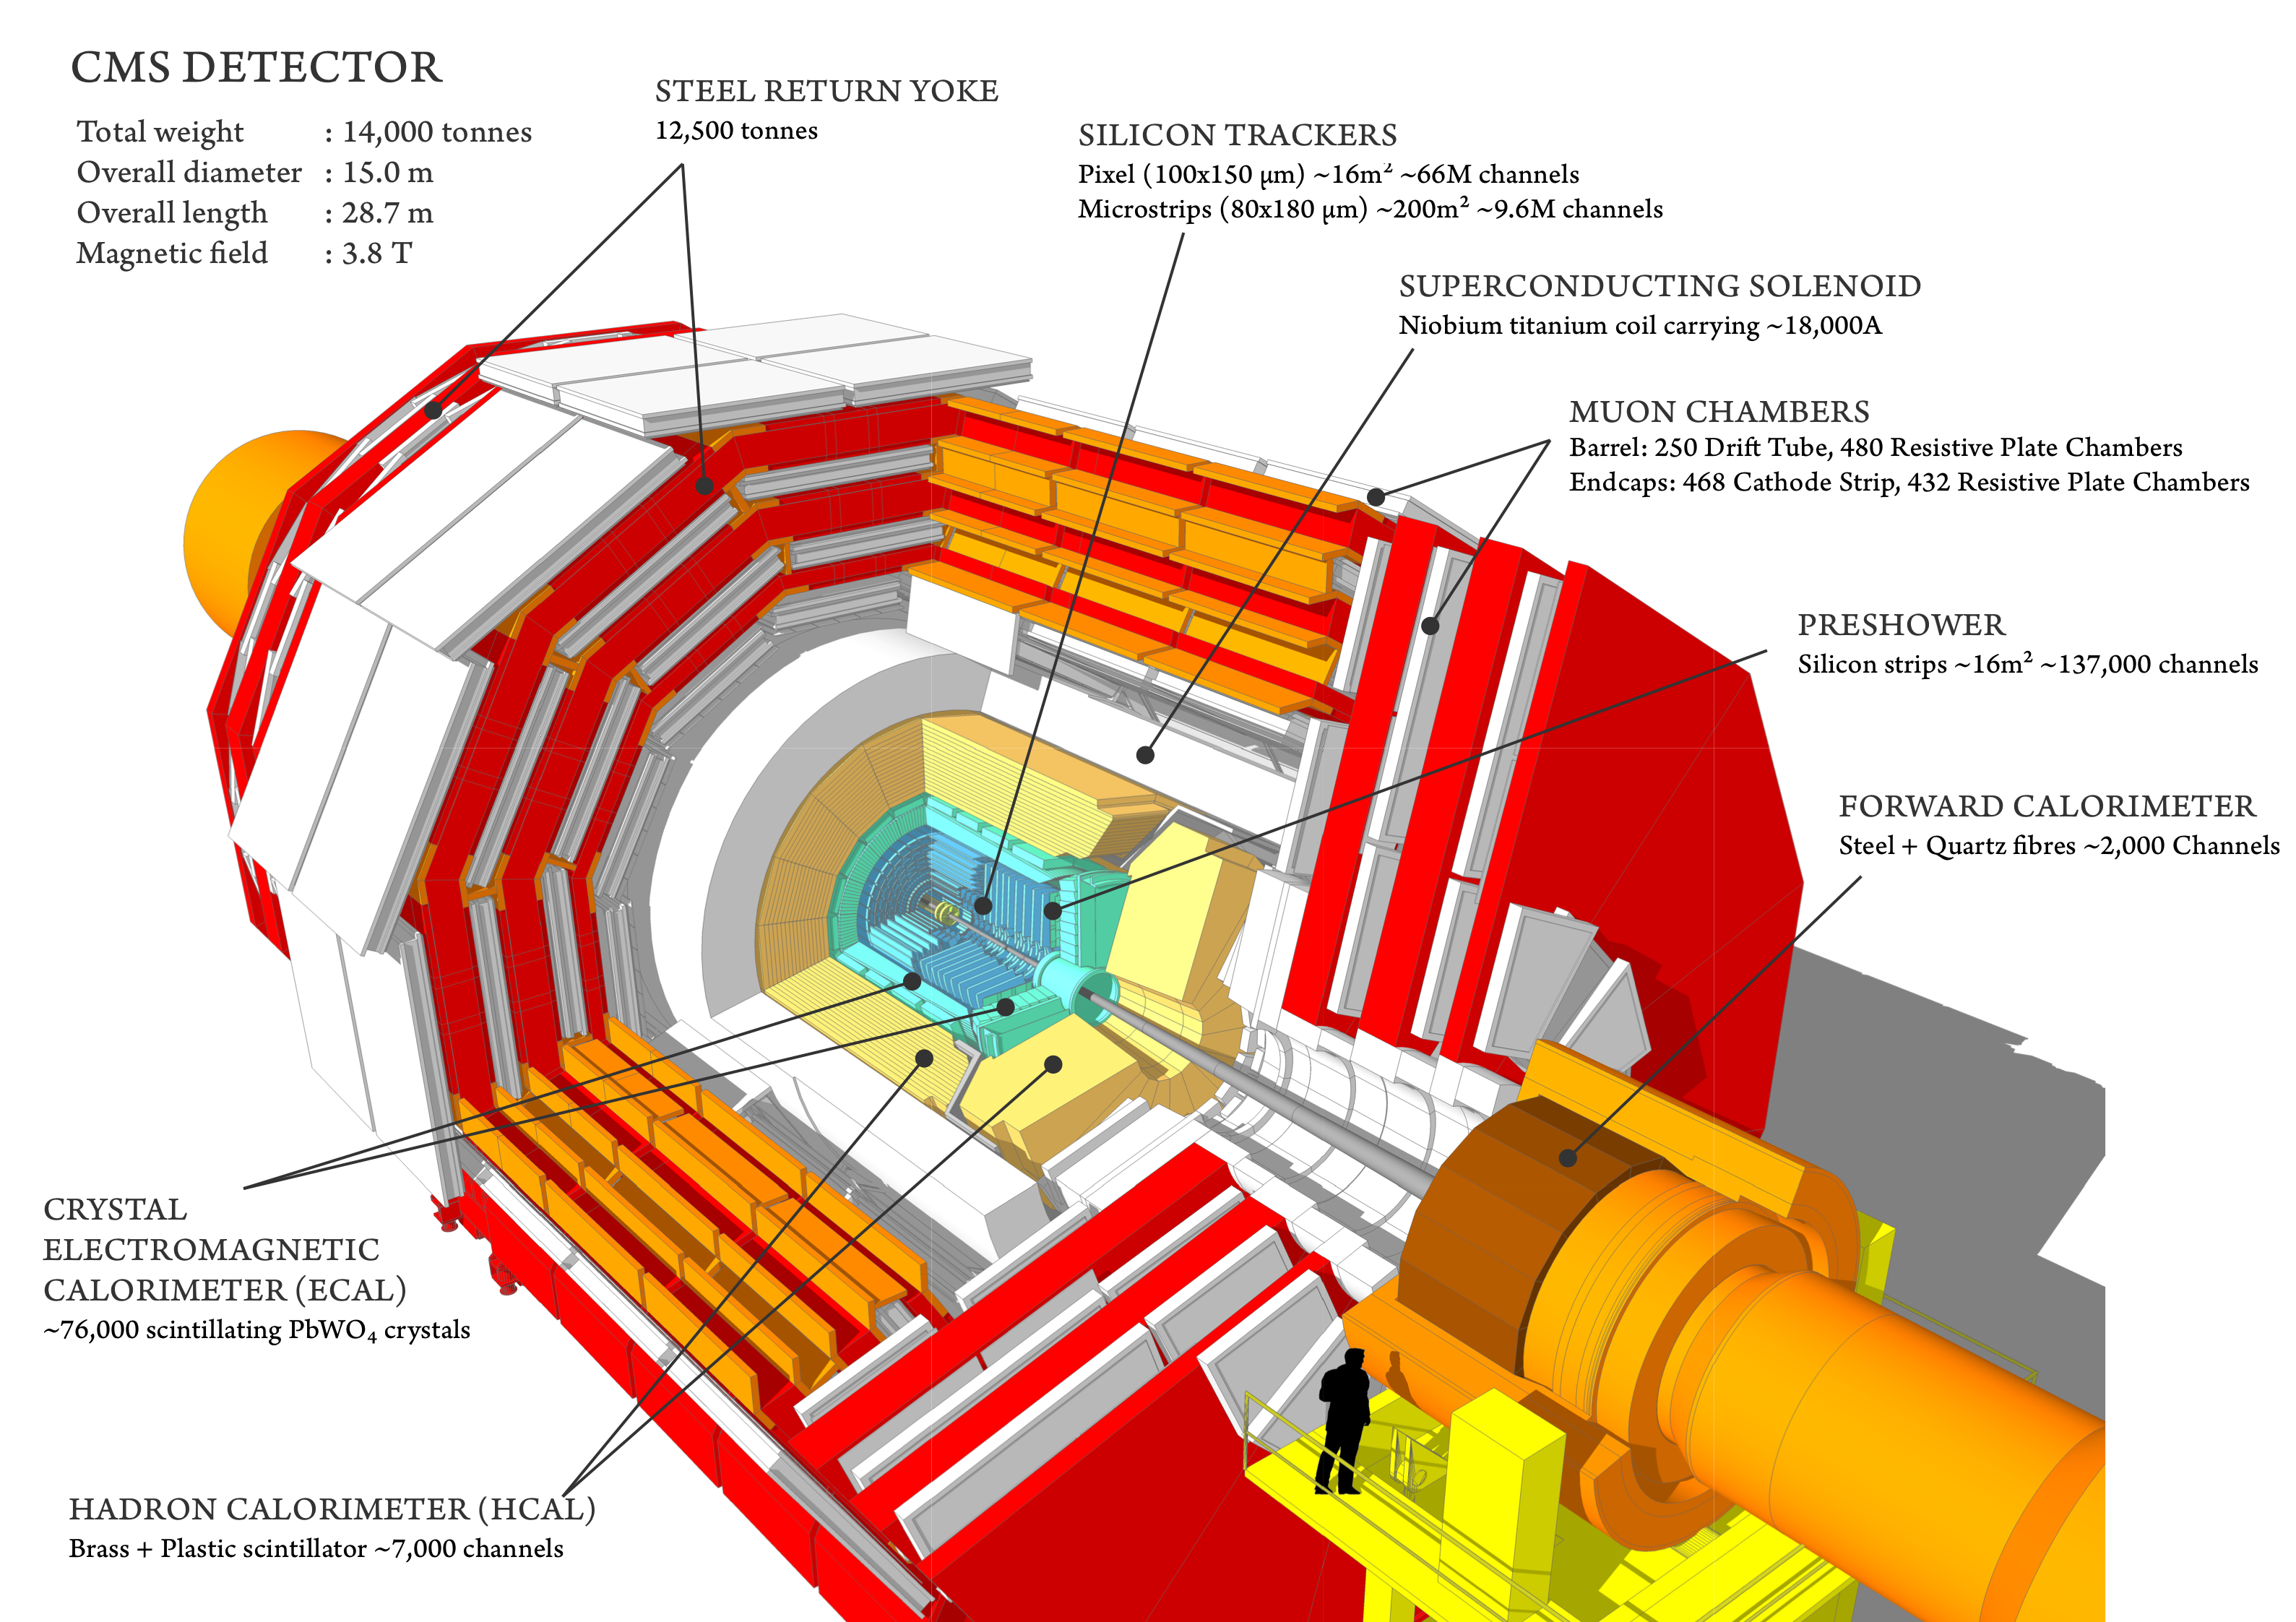
\includegraphics[width=1\textwidth]{cms.png}
	\caption{Schemat budowy detektora CMS.}
	\label{fig:cms}
	\end{figure}
	
	Detektor krzemowy, pokrywający przedział pseudopospieszności\footnote{Pseudopospieszność $\eta$ cząstki definiowana jest jako $\eta = -\ln \tg(\theta/2)$, gdzie $\theta$ to kąt między kierunkiem lotu cząstki a kierunkiem wiązki.} $|\eta| < 2.5$, składa się z dwóch rodzajów detektorów: pikselowych i paskowych. Korpus centralny składa się z trzech warstw detektorów pikselowych oraz jedenastu warstw detektorów paskowych, natomiast końcówki z jedenastu dysków, z czego dwa zawierają detektory pikselowe, a pozostałe detektory paskowe \cite{cms_technical}. Tor lotu hadronów jest rekonstruowany ze skutecznością 80-90\% w zależności od pędu poprzecznego i pseudopospieszności $\eta$. Detektory krzemowe mają grubość od 0.4 do 2.0 długości drogi radiacyjnej ($X_0$), także fotony z dużym prawdopodobieństwem konwertują wewnątrz detektora na pary $e^+e^-$ \cite{tauid13}.
	
	Kalorymetr ECAL jest zrobiony ze scyntylacyjnych kryształów stolzytu (PbWO$_4$). Posiada ponad 61000 kryształów w korpusie centralnym, pokrywającym $|\eta| < 1.48$ oraz ponad 7300 kryształów na końcach detektora, pokrywających $|\eta| < 3.0$. Stolzyt posiada krótką drogę radiacyjną ($X_0 = 0.89$ cm) oraz szybko wyświeca światło (80\% światła jest wyświecane w 25 ns). Dzięki temu dobrze rozdziela kaskady, więc jest często wykorzystywany do budowy kalorymetrów \cite{cms_technical}.
	
	Na zewnątrz ECAL znajduje się kalorymetr hadronowy HCAL zawierający mosiądz i plastik. Mosiądz został wybrany ze względu na krótką drogę swobodną (ang. \textit{interaction length}) hadronów oraz słabe właściwości magnetyczne.
Tak samo jak ECAL pokrywa obszar $|\eta| < 3.0$. Jego grubość to od siedmiu do jedenastu dróg swobodnych w zależności od $\eta$. Natomiast dla $3.0 < \eta < 5.0$ używany jest stalowo kwarcowy kalorymetr przedni (ang. \textit{Hadron Forward}) \cite{cms_technical}.
	
	Detektor mionowy składa się z trzech rodzajów komór gazowych. W części centralnej ($|\eta| < 1.2$) używane są komory \textit{drift tube} (DT), w części końcowej ($|\eta| < 2.4$), pole magnetyczne nadal jest duże, ale niejednolite, używa się \textit{cathode strip chambers} (CSC). Dodatkowo we wszystkich miejscach są zastosowane \textit{resistive plate chambers} (RPC). RPC zapewnia dobrą dokładność czasową, natomiast DT i CSC dobrą dokładność pozycyjną \cite{cms_technical}.	
	
	\section{Sieci neuronowe}
	Sieci neuronowe to klasa modeli uczenia maszynowego stosowana w uczeniu nadzorowanym \cite{dl}. Na podstawie danych treningowych zawierający zmienne objaśniające i objaśniane model uczy się zależności występujących między tymi zmiennymi. Dzięki temu możliwe jest stosowanie modelu do predykcji zmiennych objaśnianych na podstawie nowych obserwacji.
	
	Sieci neuronowe składają się z warstw. Podstawową warstwą używaną w sieciach neuronowych jest warstwa gęsta (ang. \textit{dense layer} lub \textit{fully connected layer}). Warstwa gęsta przyjmuje na wejściu wektor, a na wyjściu zwraca nowy wektor ustalonej wielkości, niekoniecznie tego samego rozmiaru. Jest to warstwa bardzo generyczna, jednak jej minusem jest duża liczba parametrów. Każda warstwa gęsta składa się z dwóch podstawowych elementów: transformacji liniowej oraz funkcji nieliniowej, zwanej funkcją aktywacji. Każda transformacja liniowa posiada wagi $w_i$ oraz przesunięcia $b_i$ (ang. \textit{bias}). Wyjście z warstwy definiowane jest jako: $$y = f(x^TW + b),$$ gdzie $x$ to wektor wejściowy, $f$ - funkcja aktywacji, nie zmieniająca wymiaru wektora, $W$ - macierz wag warstwy, $b$ - wektor przesunięcia. Dodanie kolejnych warstw to złożenie kolejnych takich funkcji.
	
	 Przykładowo na rysunku \ref{fig:simple} widoczne jest wejście do sieci $x$, które jest wektorem 3-elementowym. Następnie jest on transponowany i przemnażany przez macierz wag $W_1$, która jest wymiaru $3\times4$ oraz dodane jest przesunięcie $b_1$ o wymiarze $1\times4$. Na tym etapie nakłada się również funkcję aktywacji $f_1$. Kółka w warstwie ukrytej reprezentują wyjścia transformacji liniowych już po zastosowaniu funkcji aktywacji. Kolejny krok jest analogiczny, tym razem jest to jedna regresja liniowa, czyli macierz wag $W_2$ ma wymiar $4\times1$, a przesunięcie $b_2$ $1\times1$. Zatem wyjście~$y$: $$y = f_2\left(\left(f_1(x^TW_1 + b_1)\right)^TW_2 + b_2\right),$$ gdzie $f_1, f_2$ to funkcje aktywacji. Zauważmy, że nieliniowe funkcje aktywacji są konieczne, gdyż inaczej wielowarstwową sieć neuronową zawsze dałoby się sprowadzić do przypadku zwykłej transformacji liniowej odpowiednio przemnażając wagi \cite{dl}.
	
	\begin{figure}[H]
	\centering
	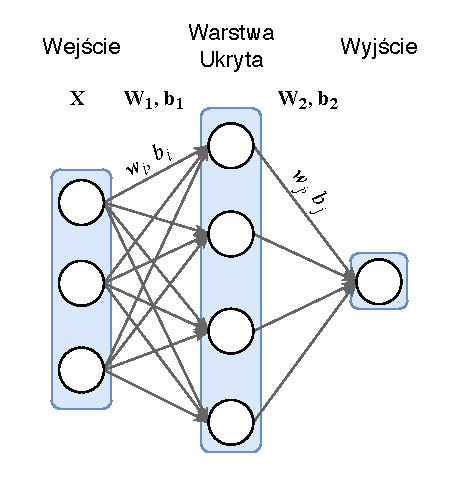
\includegraphics[width=0.5\textwidth]{simple_nn.pdf}
	\caption{Przykładowa sieć neuronowa z jedną ukrytą warstwą gęstą.}
	\label{fig:simple}
	\end{figure}
	
	Następnie aby otrzymać optymalny model poszukiwane jest minimum pewnej funkcji straty $L$ (czyli miejsce, gdzie model najmniej się myli). Przez funkcję straty rozumiana jest funkcja przybliżająca błąd popełniany przez model. Minimum jest znajdowane przy użyciu gradientu funkcji $L$ względem parametrów modelu. Niestety nie da się wyznaczyć gradientu $L$ w każdym miejscu, ale można go znaleźć w punkcie, gdzie dokonywana jest predykcja. Także, aby poprawić wagi oraz przesunięcie w modelu używa się iteracyjnego algorytmu \textit{Gradient Descent}, który polega na obliczeniu gradientu funkcji straty po parametrach modelu $\nabla_{w_i}L$, a następnie aktualizowane są wagi o pewien krok w kierunku ujemnego gradientu, także dla przykładowej wagi $w$ przy $n+1$-szej iteracji (górny indeks oznacza numer iteracji): $$w^{(n+1)} \leftarrow w^{(n)} - \gamma \frac{\partial L^{(n)}}{\partial w^{(n)}},$$ gdzie $\gamma$ to tzw. stała uczenia (ang. \textit{learning rate}) \cite{dl}. Widać, że istotne jest aby wszystkie funkcje użyte w modelu były różniczkowalne prawie wszędzie (w punktach nieciągłości pochodnej można przyjąć dowolną wartość brzegową). 
	
	\begin{figure}
	\centering
	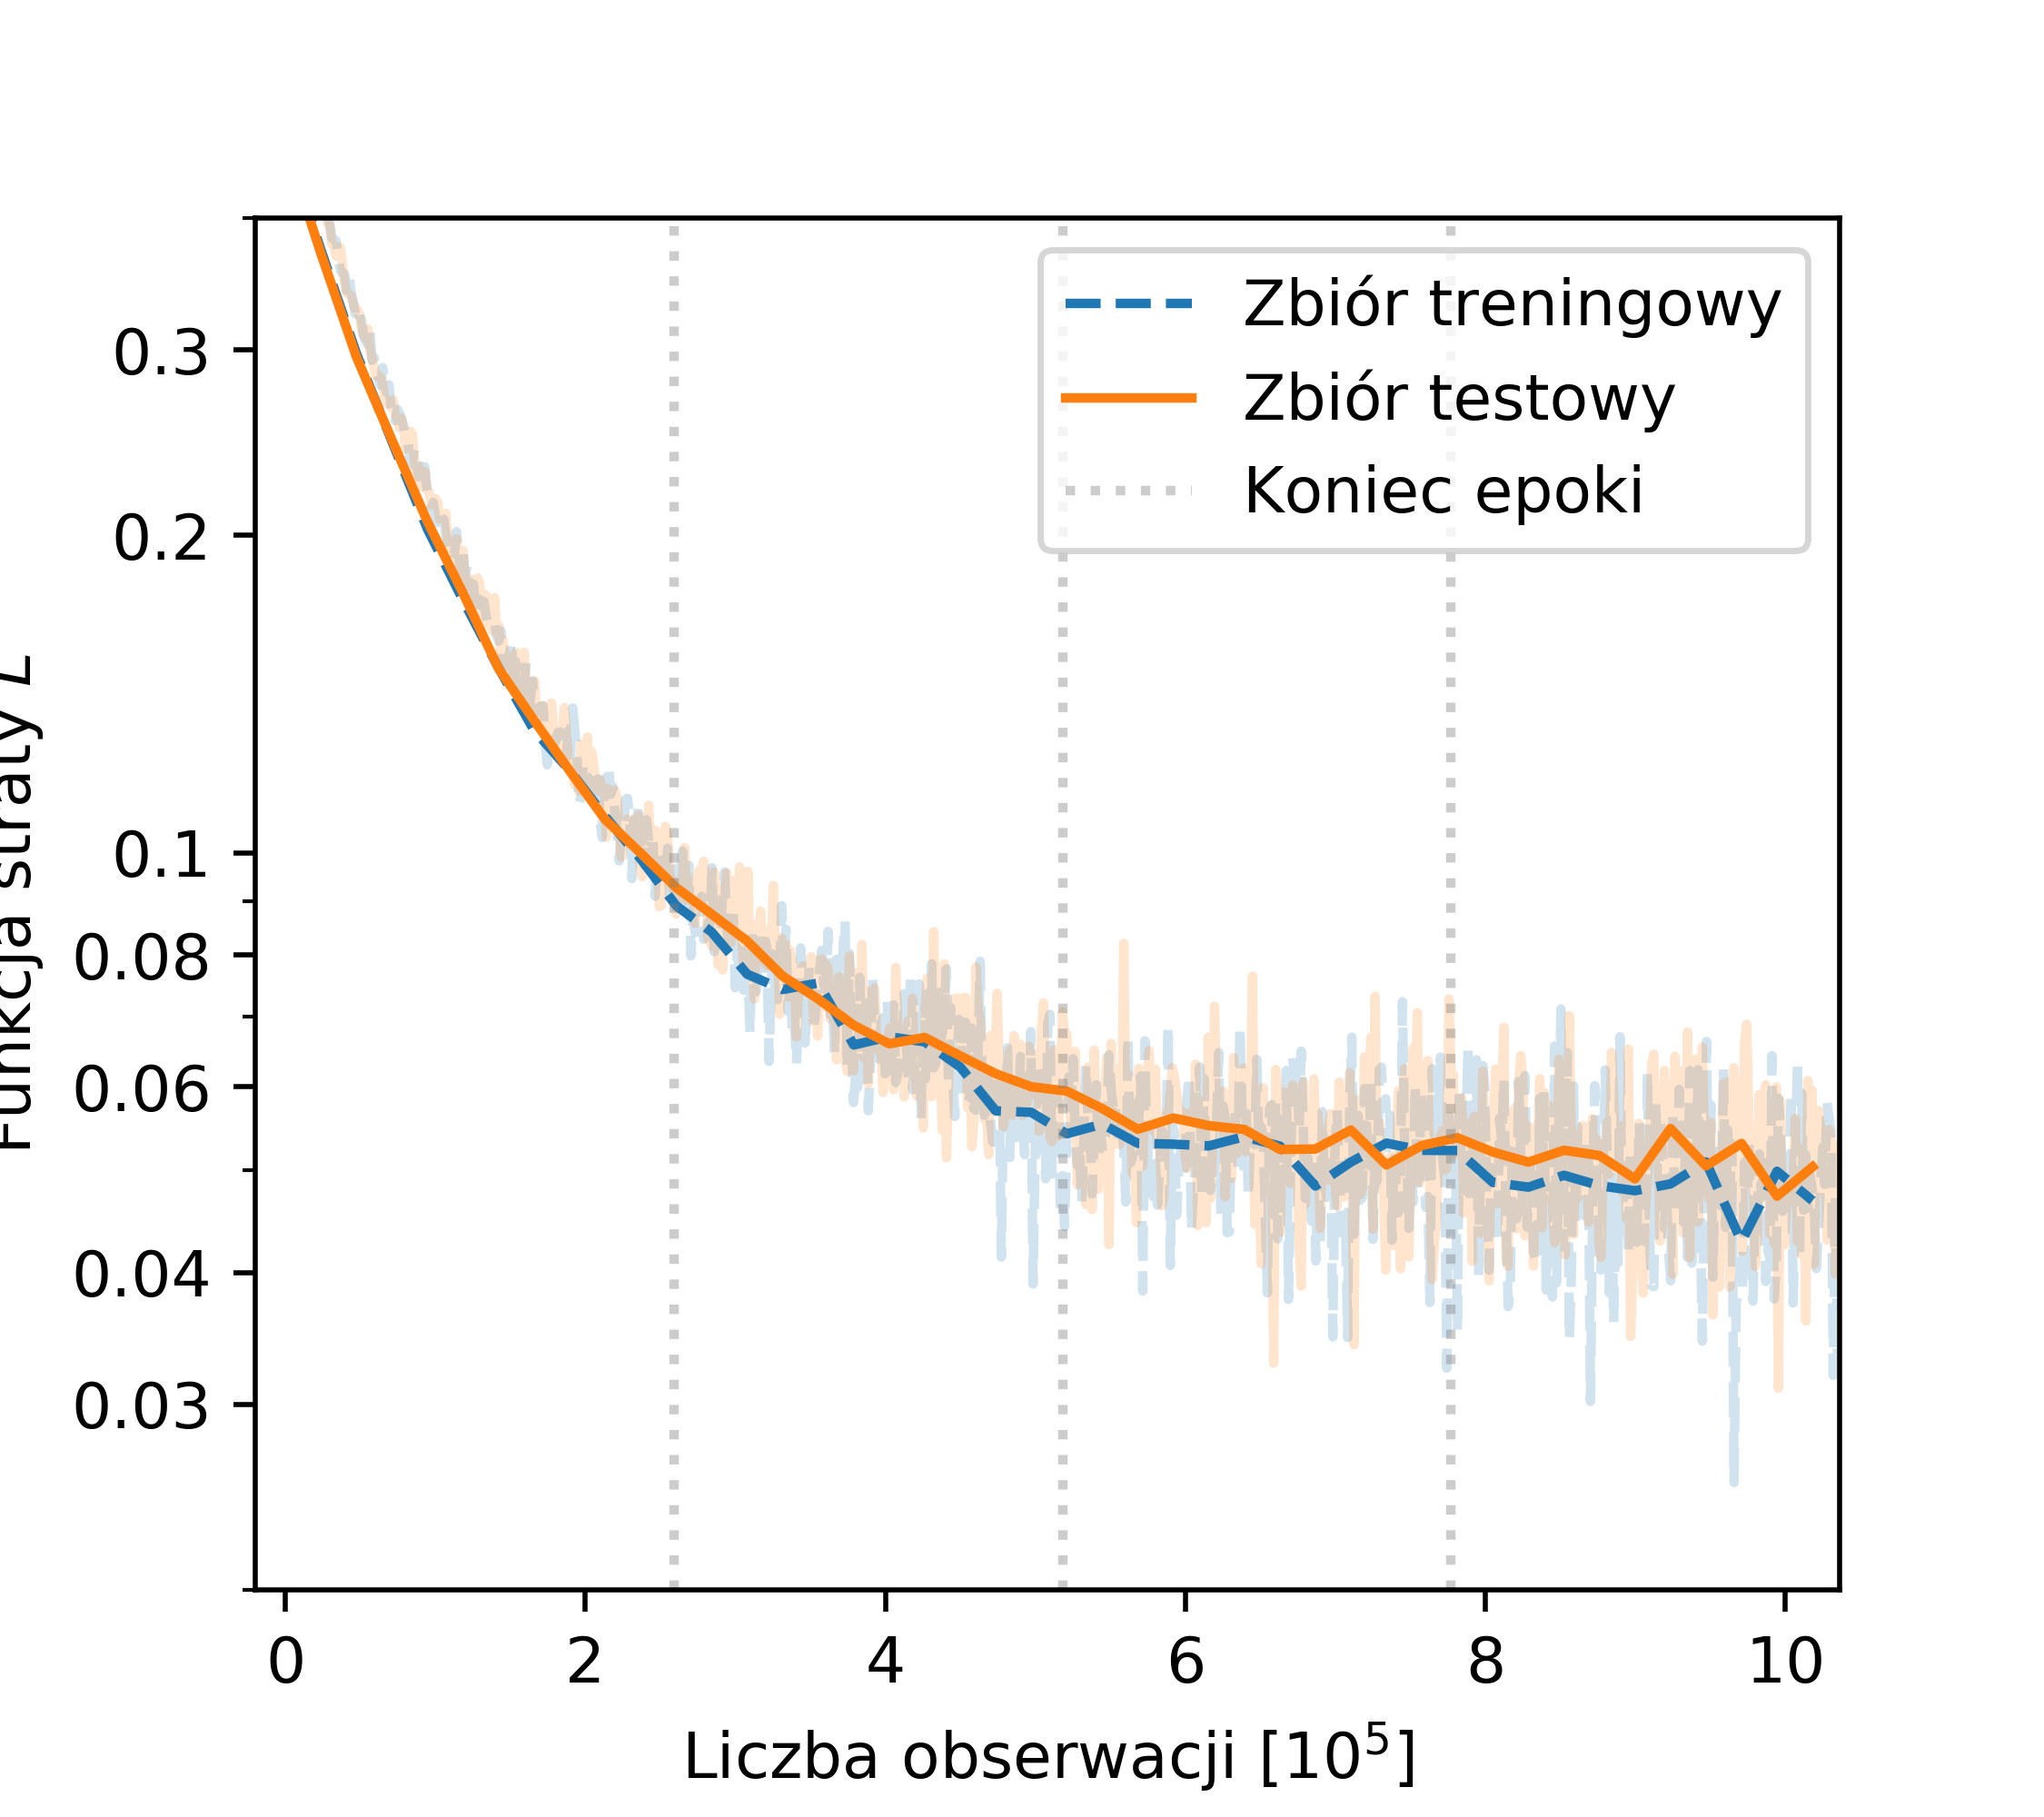
\includegraphics[width=0.7\textwidth]{loss_ensemble.png}
	\caption{Przykładowa zmiana funkcji straty dla zbioru treningowego i testowego od liczby obserwacji, pionowymi liniami zaznaczono końce kolejnych epok.}
	\label{fig:loss_example}
	\end{figure}	
	
	W praktyce sieci neuronowe uczone są algorytmem \textit{Stochastic Gradient Descent} (SGD). Polega on na liczeniu funkcji straty dla pewnej liczby obserwacji (zwanej później \textit{batchem}), zamiast dla wszystkich obserwacji. Jednorazowe przejście przez wszystkie obserwacje nazywane jest epoką, a zazwyczaj trening modelu składa się z wielu epok. Przykładowy wygląd krzywej uczenia, czyli wykresu funkcji straty od liczby obserwacji przedstawiony jest na rysunku \ref{fig:loss_example}.
	
	Rozwinięciem algorytmu SGD jest algorytm \textit{Adam} (\textit{Adaptive momentum}) \cite{adam}, który pomaga w zapobieganiu pozostawania w lokalnych minimach funkcji straty.
	
	\subsection{Funkcje aktywacji}
	Stosowane później funkcje aktywacji wraz ze wzorami:
	\begin{itemize}
	\item Sigmoid: $$S(x) = \frac{1}{1+e^{-x}},$$
	\item ReLU\cite{relu} $$ReLU(x) = \max(0, x).$$
	\end{itemize}
	
	\subsection{Warstwa \textit{batch normalization}}
	Wraz z postępem w treningu sieci wyjścia z warstw sieci mogą się zmieniać. W szczególności rozkład wyjścia może ulec zmianie, do czego każda następna warstwa sieci musi się na nowo dostosowywać. Przeciwdziała temu warstwa \textit{batch normalization}, która przeskalowuje każdy batch tak aby miał tą samą średnią i odchylenie standardowe \cite{batch_norm}. Dzięki zastosowaniu \textit{batch normalization} trening sieci trwa krócej, a sieć może osiągnąć lepszą skuteczność.
	
	\subsection{Harmonogram stałej uczenia}
	Poza dopasowywaniem wielkości kroku aktualizacji wag zastosowanym w algorytmie \textit{Adam}, stosuje się harmonogram stałej uczenia. Polega on na zmniejszaniu stałej uczenia, gdy występuje wypłaszczenie krzywej uczenia. Jeśli funkcja straty nie zmniejsza się przez określoną liczbę epok, stała uczenia zmniejszana jest o pewien czynnik aż osiągnie zadaną wcześniej wartość minimalną.
	
	\section{XGBoost}
	W uczeniu maszynowym przez drzewo decyzyjne rozumie się model statystyczny dokonujący predykcji na podstawie sekwencji binarnych decyzji (rysunek \ref{fig:tree}). W praktyce pojedyncze drzewo decyzyjne jest rzadko stosowane ze względu na niską skuteczność predykcyjną. W zamian używane są algorytmy, które budują wiele drzew decyzyjnych i agregują ich wyniki.
	
	 Jednym z nich jest XGBoost (\textit{eXtreme Gradient Boosting}) \cite{xgboost}, który jest implementacją algorytmu \textit{Gradient Boosting}. W pierwszym kroku budowane jest pojedyncze drzewo decyzyjne, które możliwie najlepiej przewiduje zmienną objaśnianą. Następnie, każde kolejne drzewo jest tworzone aby jak najlepiej przewidywać błąd popełniany przez poprzedni zestaw drzew. Końcowa predykcja to suma wszystkich odpowiedzi drzew.
	
	\begin{figure}[h]
	\centering
	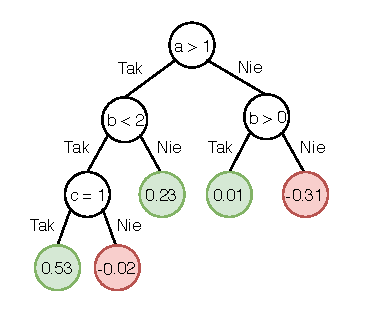
\includegraphics[width=0.5\textwidth]{tree.pdf}
	\caption{Przykładowe drzewo decyzyjne, $a, b, c$ to zmienne występujące w danych}
	\label{fig:tree}
	\end{figure}
	
	\section{Miary skuteczności modeli}
	Jako, że identyfikacja taonów to problem klasyfikacji binarnej, dobrą metryką do mierzenia skuteczności modelu jest ROC AUC (\textit{Area Under Receiver Operating Characteristic Curve}) oraz sama krzywa ROC. Analizowany model przewiduje prawdopodobieństwo, czy dany rozpad zawiera taon. Aby dokonać klasyfikacji musimy ustalić próg odcięcia ponad którym zawsze zwracane jest 1 (wystąpił taon), a poniżej 0 (nie wystąpił). Wówczas można policzyć prawdziwe pozytywa (ang. \textit{true positives}, TP), czyli obserwacje oznaczone w danych jako sygnał i przewidziane jako sygnał oraz fałszywe pozytywa (ang. \textit{false positives}, FP), czyli obserwacje oznaczone w danych jako tło, a przewidziane jako sygnał. Następnie można obliczyć \textit{true positive rate} (TPR), czyli TP podzielone przez liczbę wszystkich obserwacji oznaczonych w danych jako sygnał oraz \textit{false positive rate} (FPR), czyli FP podzielone przez liczbę wszystkich obserwacji oznaczonych w danych jako tło. Krzywa ROC to wykres TPR od FPR dla różnych progów odcięcie. Jednak zgodnie z występującą w fizyce cząstek konwencją, na wykresach krzywej ROC osie są zamienione, zatem jest to wykres FPR od TPR. 
	
	ROC AUC to pole pod krzywą ROC. W związku z tym przyjmuje ona wartości pomiędzy 0 a 1, gdzie 0.5 to wartość osiągana przez model losowy (przewidującego losowe prawdopodobieństwo np. z rozkładu jednostajnego od 0 do 1), zaś 1 przez bezbłędny klasyfikator. Przykładowa krzywa ROC oraz jej ROC AUC dla modelu losowego oraz nielosowego znajdują się na rysunku \ref{fig:roc}. ROC AUC nie jest różniczkowalna, więc nie można jej bezpośrednio wykorzystać przy treningu sieci neuronowej jako funkcji straty. Jest jednak jest przydatna przy ewaluacji oraz porównywaniu wytrenowanych modeli. 
	
	Do treningu jako funkcje straty wykorzystuje się zazwyczaj binarną entropię krzyżową (ang. \textit{binary cross entropy}) \cite{dl}, daną wzorem: $$ L(y, p) = -(y\log(p)+(1-y)\log(1-p)),$$ gdzie $y$ to prawdziwe prawdopodobieństwo, że dana obserwacja zawiera taon (0 albo 1), a $p$ to jego oszacowanie przez model.

	\begin{figure}[h]
	\centering
	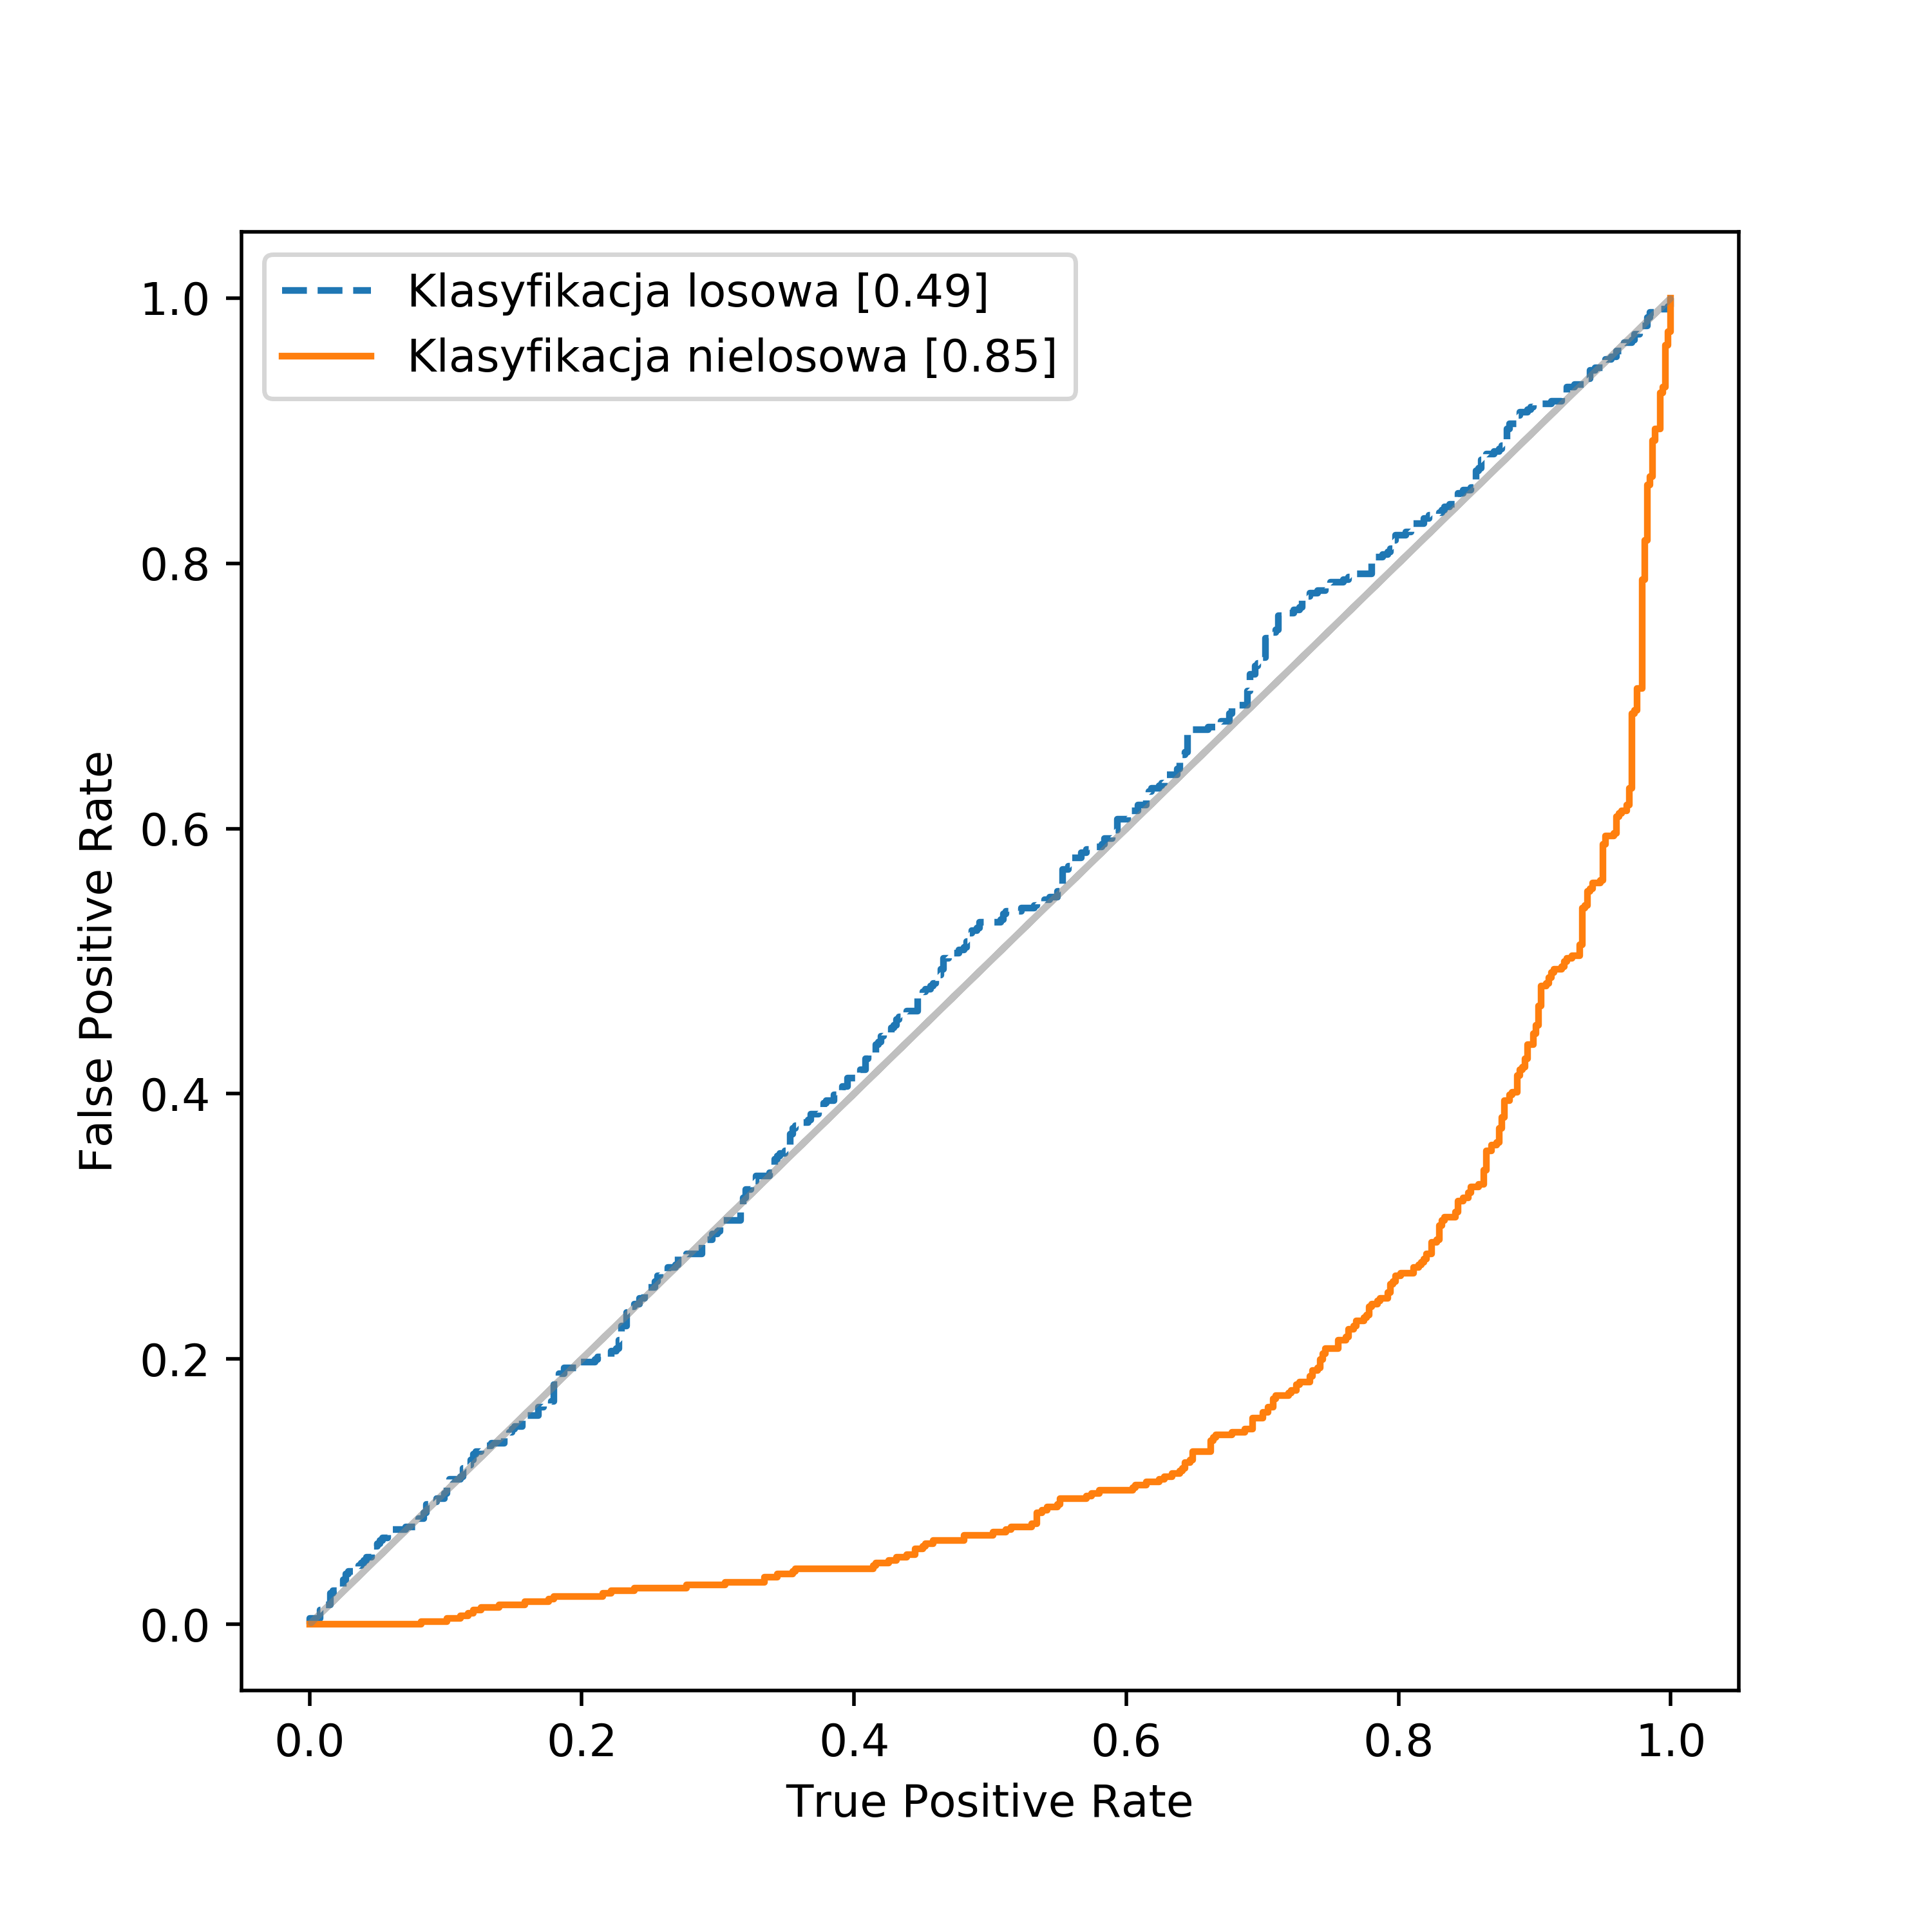
\includegraphics[width=0.8\textwidth]{roc_example.png}
	\caption{Przykładowe krzywe ROC dla klasyfikatora losowego oraz nielosowego. W nawiasach kwadratowych podano wartość ROC AUC dla danego modelu.}
	\label{fig:roc}
	\end{figure}
	
	\section{Istotność zmiennych}
	Jednym ze sposobów sprawdzenia istotności zmiennych w modelu predykcyjnym jest metoda permutacyjna \cite{breiman2001random}. Polega na losowym permutowaniu jednej zmiennej objaśniającej w zbiorze danych, a następnie mierzeniu jaką skuteczność osiąga model na takim zbiorze. Jeśli skuteczność modelu się pogorszyła, wnioskuje się, że dana zmienna jest używana przez model przy predykcji.  Po wykonaniu tej operacji dla każdej zminnej objaśniającej można uzyskać informacje które zmienne są w największym stopniu wykorzystywane przez model.
	
    \chapter{Dane symulacyjne}
    \label{ch:dane}
    Dane użyte w pracy pochodzą z symulacji zderzeń proton-proton w których został wyprodukowany bozon Higgsa i rozpadł się na parę $\tau\tau$ (szukany sygnał). Natomiast za tło zostały przyjęte dżety QCD.
	
	Przy analizowaniu rozpadów taonów wydziela się części przestrzeni, które są potencjalnie bardziej interesujące. Takimi częściami są stożek sygnału (ang. \textit{signal cone}) oraz stożek izolacji (ang. \textit{isolation cone}). W stożku sygnału powinny znajdować się jedynie produkty rozpadu taonu. Na rysunku \ref{fig:cones} znajduje się przykładowy rozpad taonu z zaznaczonym stożkiem sygnałowym oraz izolacji.

	\begin{figure}[H]
	\centering
	\includegraphics[width=0.5\textwidth]{cones.pdf}
	\caption{Przykładowy schemat rozpadu taonu z zaznaczonym stożkiem sygnałowym oraz izolacji.}
	\label{fig:cones}
	\end{figure}

\newpage    
Dane są wstępnie przetwarzane tak, aby pozostawić tylko najbardziej potrzebne informacje. Ostatecznie, otrzymane dane mają 19 zmiennych objaśniających \cite{cms2016reconstruction}:

	\begin{itemize}
	\item \textbf{byCombinedIsolationDeltaBetaCorrRaw3Hits} - Suma pędów cząstek naładowanych oraz fotonów wewnątrz stożka izolacji pomniejszona o korektę $\Delta\beta$, zapisuje się wzorem:  $$I_{\tau} = \sum p_T^{\mathrm{charged}}(d_z < 0.2 \mathrm{cm}) + \mathrm{max}(0, \sum p^{\gamma}_T - \Delta\beta)$$.
	\item \textbf{chargedIsoPtSum} - Suma pędów naładowanych produktów rozpadu wewnątrz stożka sygnałowego.
	\item \textbf{decayDistMag} - Odległość między zderzeniem $pp$ a punktem, w którym nastąpił rozpad taonu.
	\item \textbf{decayMode} - Kanał rozpadu taonu.
	\item \textbf{dxy} - Odległość między zderzeniem $pp$ a punktem, w którym nastąpił rozpad taonu w rzucie na płaszczyznę prostopadłą do osi wiązki.
	\item \textbf{dxy\_Sig} - Zmienna \textbf{dxy} podzielona przez niepewność pomiaru.
	\item \textbf{eRatio} - Stosunek energii elektromagnetycznej do całkowitej energii całkowitej produktów rozpadu.
	\item \textbf{flightLengthSig} - Zmienna \textbf{decayDistMag} podzielona przez niepewność pomiaru. 
	\item \textbf{gjAngleDiff} - Kąt między kierunkiem ruchu taonu oraz kierunkiem ruchu wiodącego produktu rozpadu.
	\item \textbf{hasSecondaryVertex} - Informacja czy rozpad posiada wierzchołek wtórny, którym może być rozpad taonu.
	\item \textbf{ip3d} - Odległość między zderzeniem $pp$ a najbliższym punktem na krzywej zakreślanej przez wiodący produkt rozpadu taonu.
	\item \textbf{nPhoton} - Liczba protonów o pędzie $p_T > 0.5$ GeV przypisana do rozpadu taonu.
	\item \textbf{neutralIsoPtSum} - Suma pędów neutralnych produktów rozpadu wewnątrz stożka sygnałowego.
	\item \textbf{photonPtSumOutsideSignalCone} - Suma pędów fotonów poza stożkiem sygnałowym.
	\item \textbf{ptWeightedDetaStrip} - Suma $\Delta\eta$ ważona pędami cząstek, gdzie $\Delta\eta$ to różnica $\eta$ między taonem a produktem rozpadu taonu.
	\item \textbf{ptWeightedDphiStrip} - Suma $\Delta\phi$ ważona pędami cząstek, gdzie $\Delta\phi$ to różnica $\phi$ między taonem a produktem rozpadu taonu.
	\item \textbf{ptWeightedDrIsolation} - Suma $\Delta R$ ważona pędami cząstek wewnątrz stożka izolacji, gdzie $\Delta R = \sqrt{(\Delta\eta)^2 + (\Delta\phi)^2}$.
	\item \textbf{ptWeightedDrSignal} - Suma $\Delta R$ ważona pędami cząstek wewnątrz stożka sygnałowego.
	\item \textbf{puCorrPtSum} - Suma pędów cząstek neutralnych znajdujących się wewnątrz stożka sygnałowego, ale pochodząca z innych rozpadów.
	\end{itemize}
	
	Dodatkowo dane zawierają 4 zmienne będące odpowiedziami wcześniej wykorzystywanych klasyfikatorów do identyfikacji taonów:
	\begin{itemize}
	\item \textbf{byIsolationMVArun2v1DBnewDMwLTraw2017v2} - Model drzewiasty oparty o algorytm \textit{AdaBoost} \cite{freund1997decision}.
	\item \textbf{deepTau2017v1tauVSall} - Jeden z modeli opartych o głębokie sieci neuronowe. Używany do rozróżniania taonów od wszystkich rodzajów tła.
	\item \textbf{deepTau2017v1tauVSjet} - Jeden z modeli opartych o głębokie sieci neuronowe. Używany do rozróżniania taonów od dżetów QCD.
	\item \textbf{DPFTau\_2016\_v1tauVSall} - Jeden z modeli opartych o głębokie sieci neuronowe. W przeciwieństwie do pozostałych modeli, był trenowany na danych zawierających pojedyncze produkty rozpadu (a nie zsumowane).
	\end{itemize}
	
	Jako, że są to dane symulacyjne, występuje tam również informacja o wystąpieniu taonu, czyli zmienna objaśniania. Rozpatrujemy tylko jeden rodzaj tła, także przyjmuje ona wartość 1 jeśli taon wystąpił (sygnał) oraz 0 jeśli był to dżet QCD (tło).
	
	Na rysunku \ref{fig:diff} przedstawiono rozkłady przykładowych zmiennych dla sygnału oraz tła. Widać zauważalne różnice w rozkładach, także można na podstawie tej zmiennej dokonywać klasyfikacji. Rozkłady częściowo się nakładają, więc klasyfikacja na podstawie żadnej ze zmiennych nie byłaby idealna.
	
	\begin{figure}
	\begin{subfigure}{.5\textwidth}
	\centering
	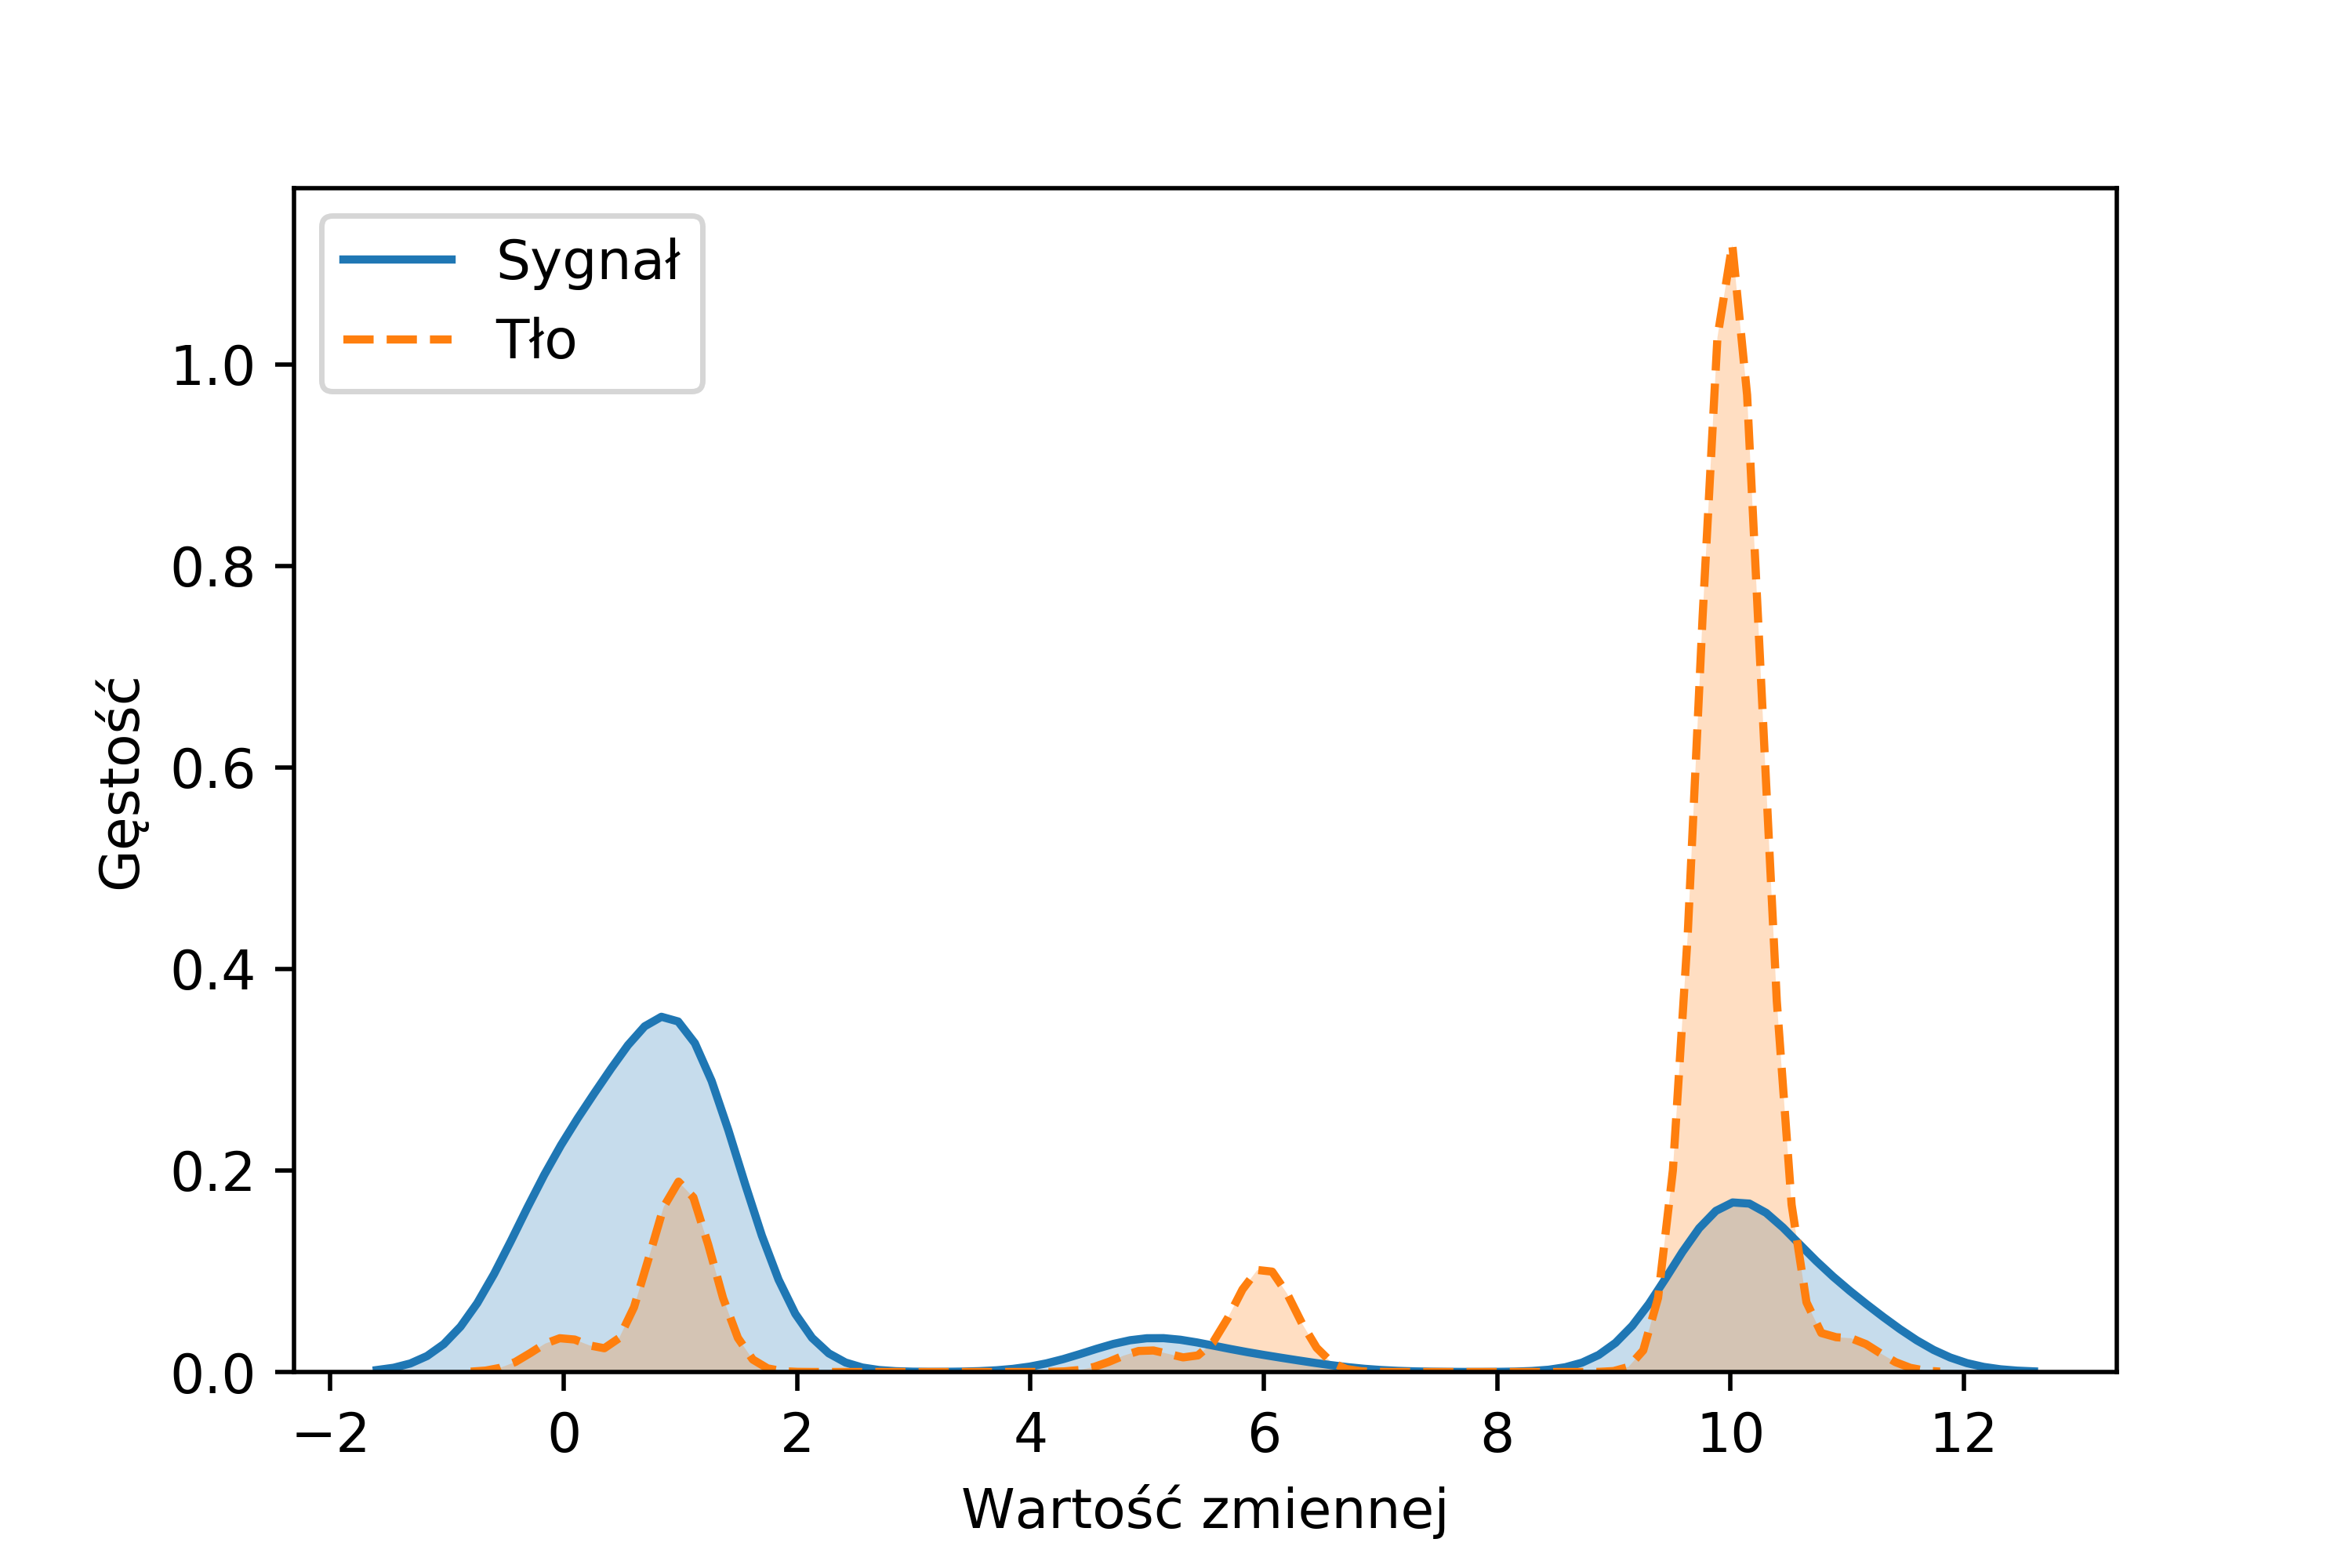
\includegraphics[width=1\textwidth]{difference_decayMode.png}
	\caption{decayMode}
	\end{subfigure}
	\begin{subfigure}{.5\textwidth}
	\centering
	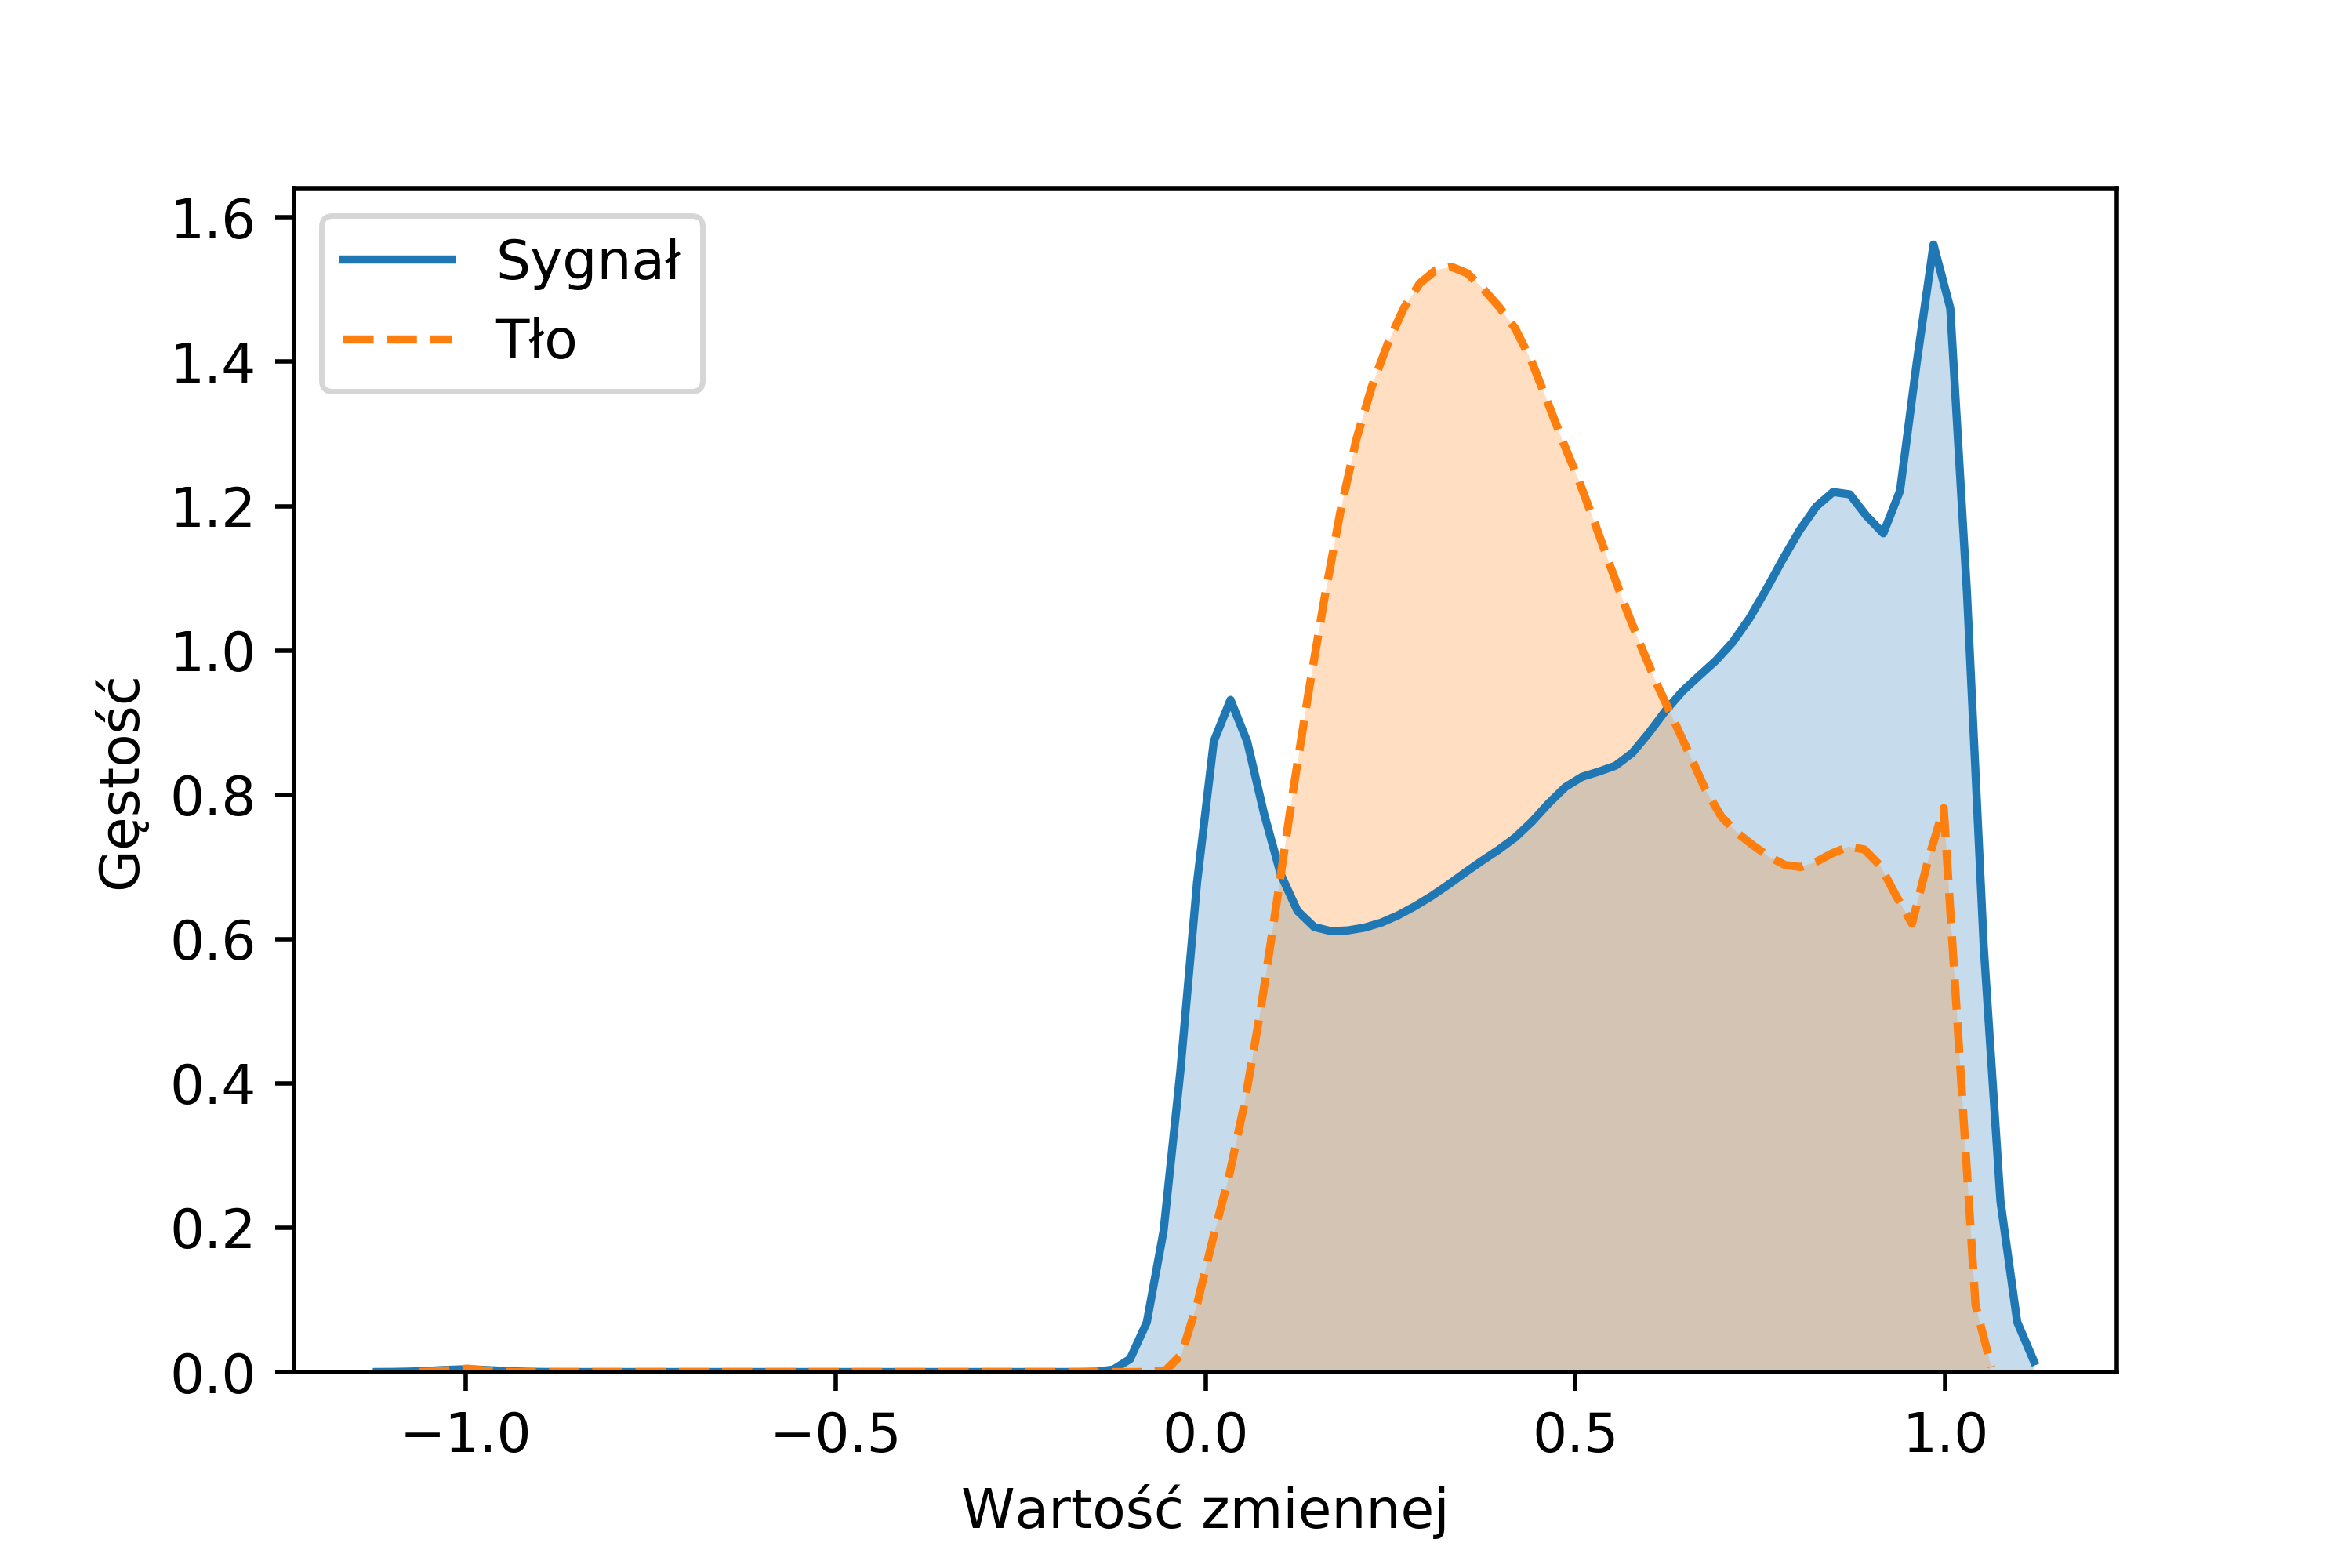
\includegraphics[width=1\textwidth]{difference_eRatio.png}
	\caption{eRatio}
	\end{subfigure}
	\begin{subfigure}{.5\textwidth}
	\centering
	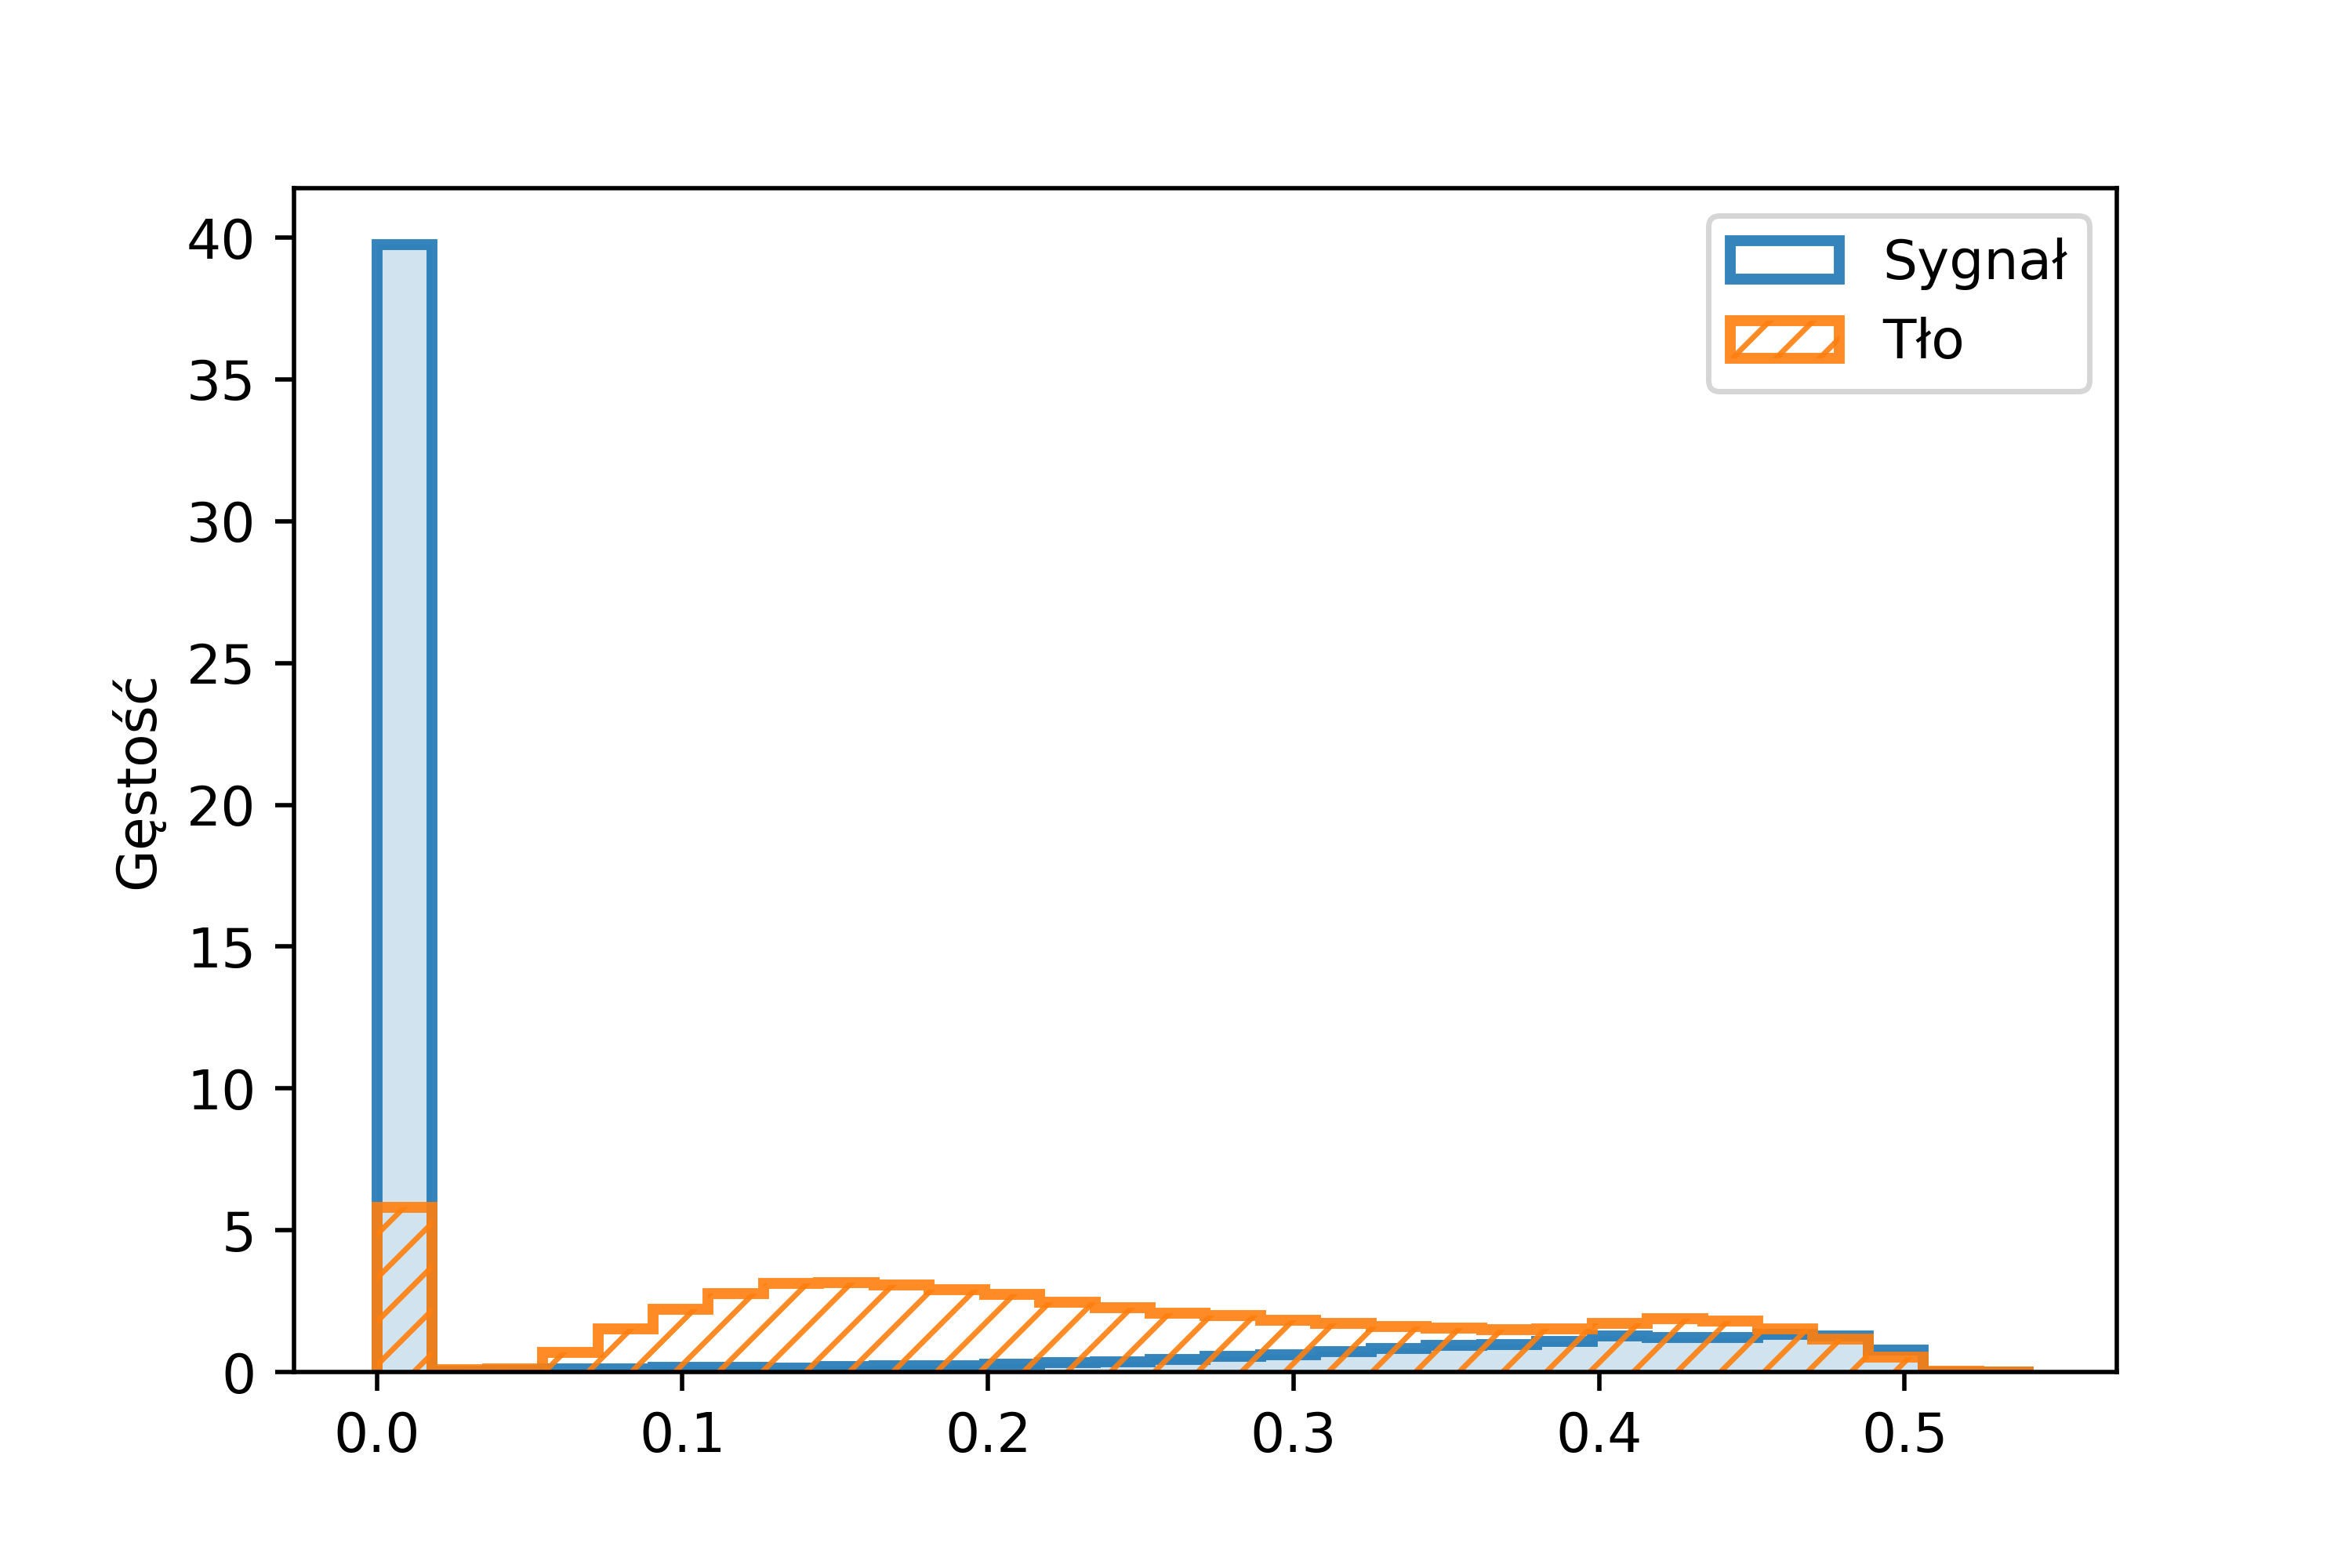
\includegraphics[width=0.95\textwidth]{difference_ptWeightedDrIsolation.png}
	\caption{ptWeightedDrIsolation}
	\end{subfigure}
	\begin{subfigure}{.5\textwidth}
	\centering
	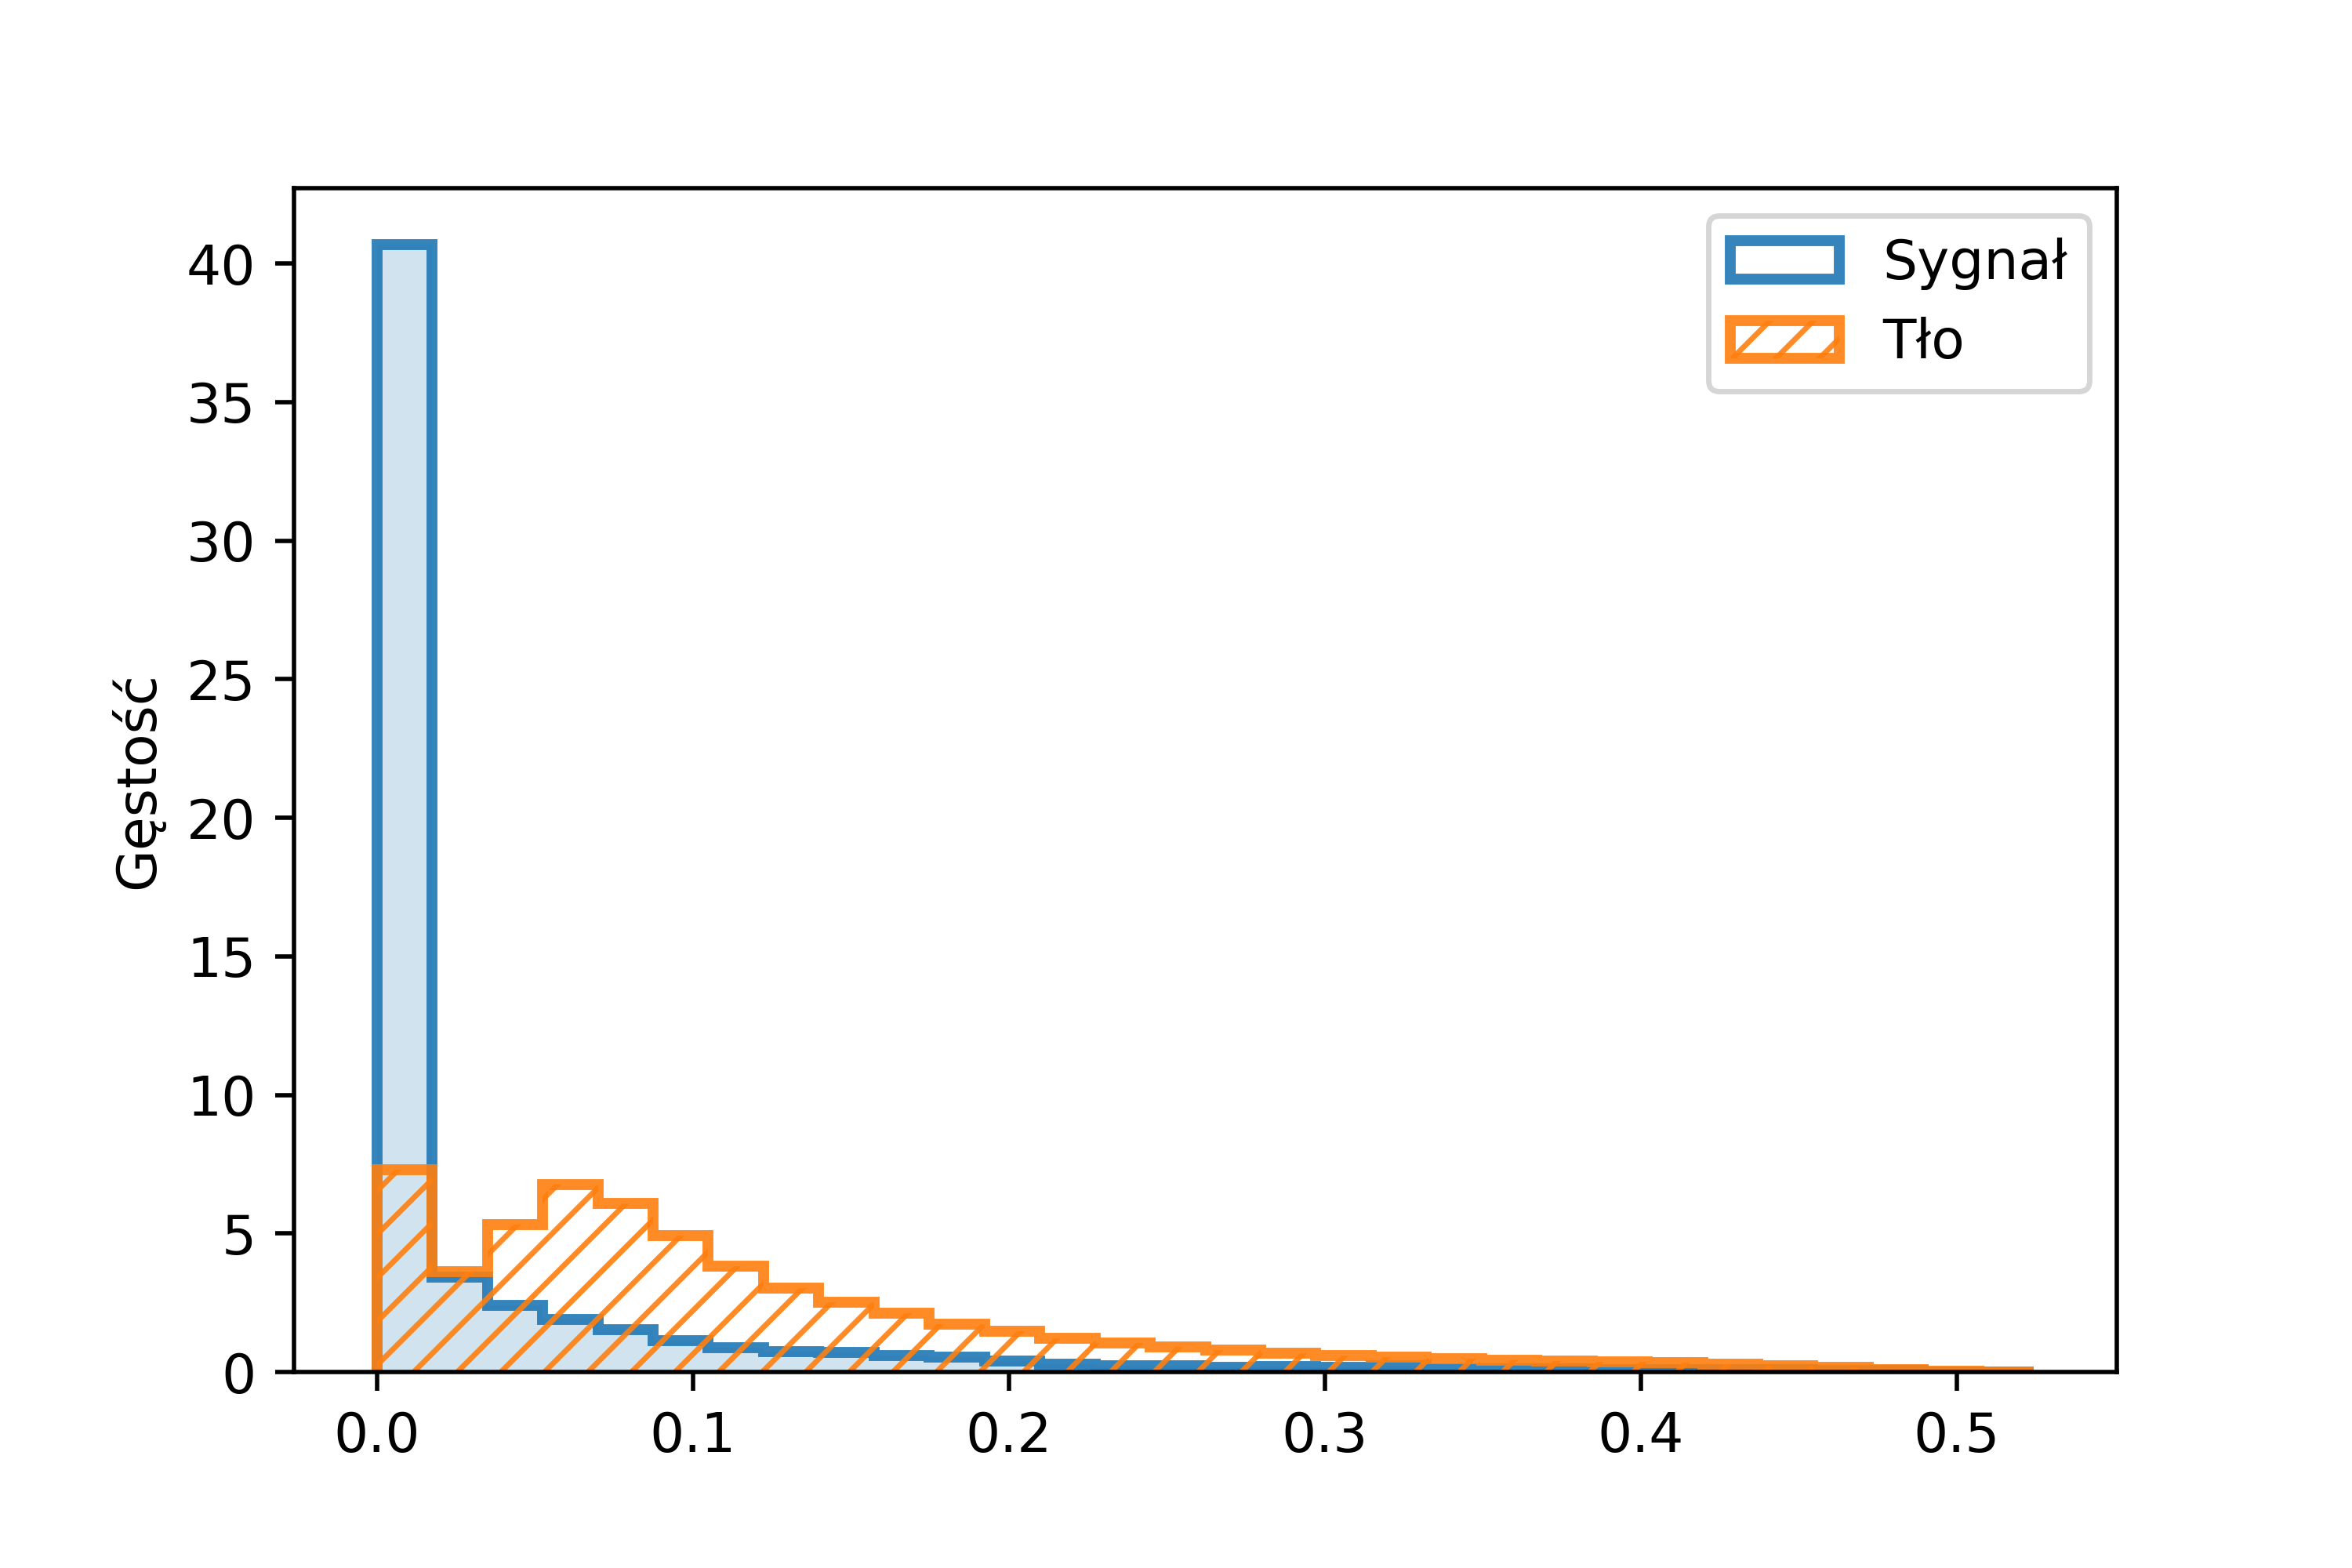
\includegraphics[width=1\textwidth]{difference_ptWeightedDetaStrip.png}
	\caption{ptWeightedDetaStrip}
	\end{subfigure}
	\begin{subfigure}{.5\textwidth}
	\centering
	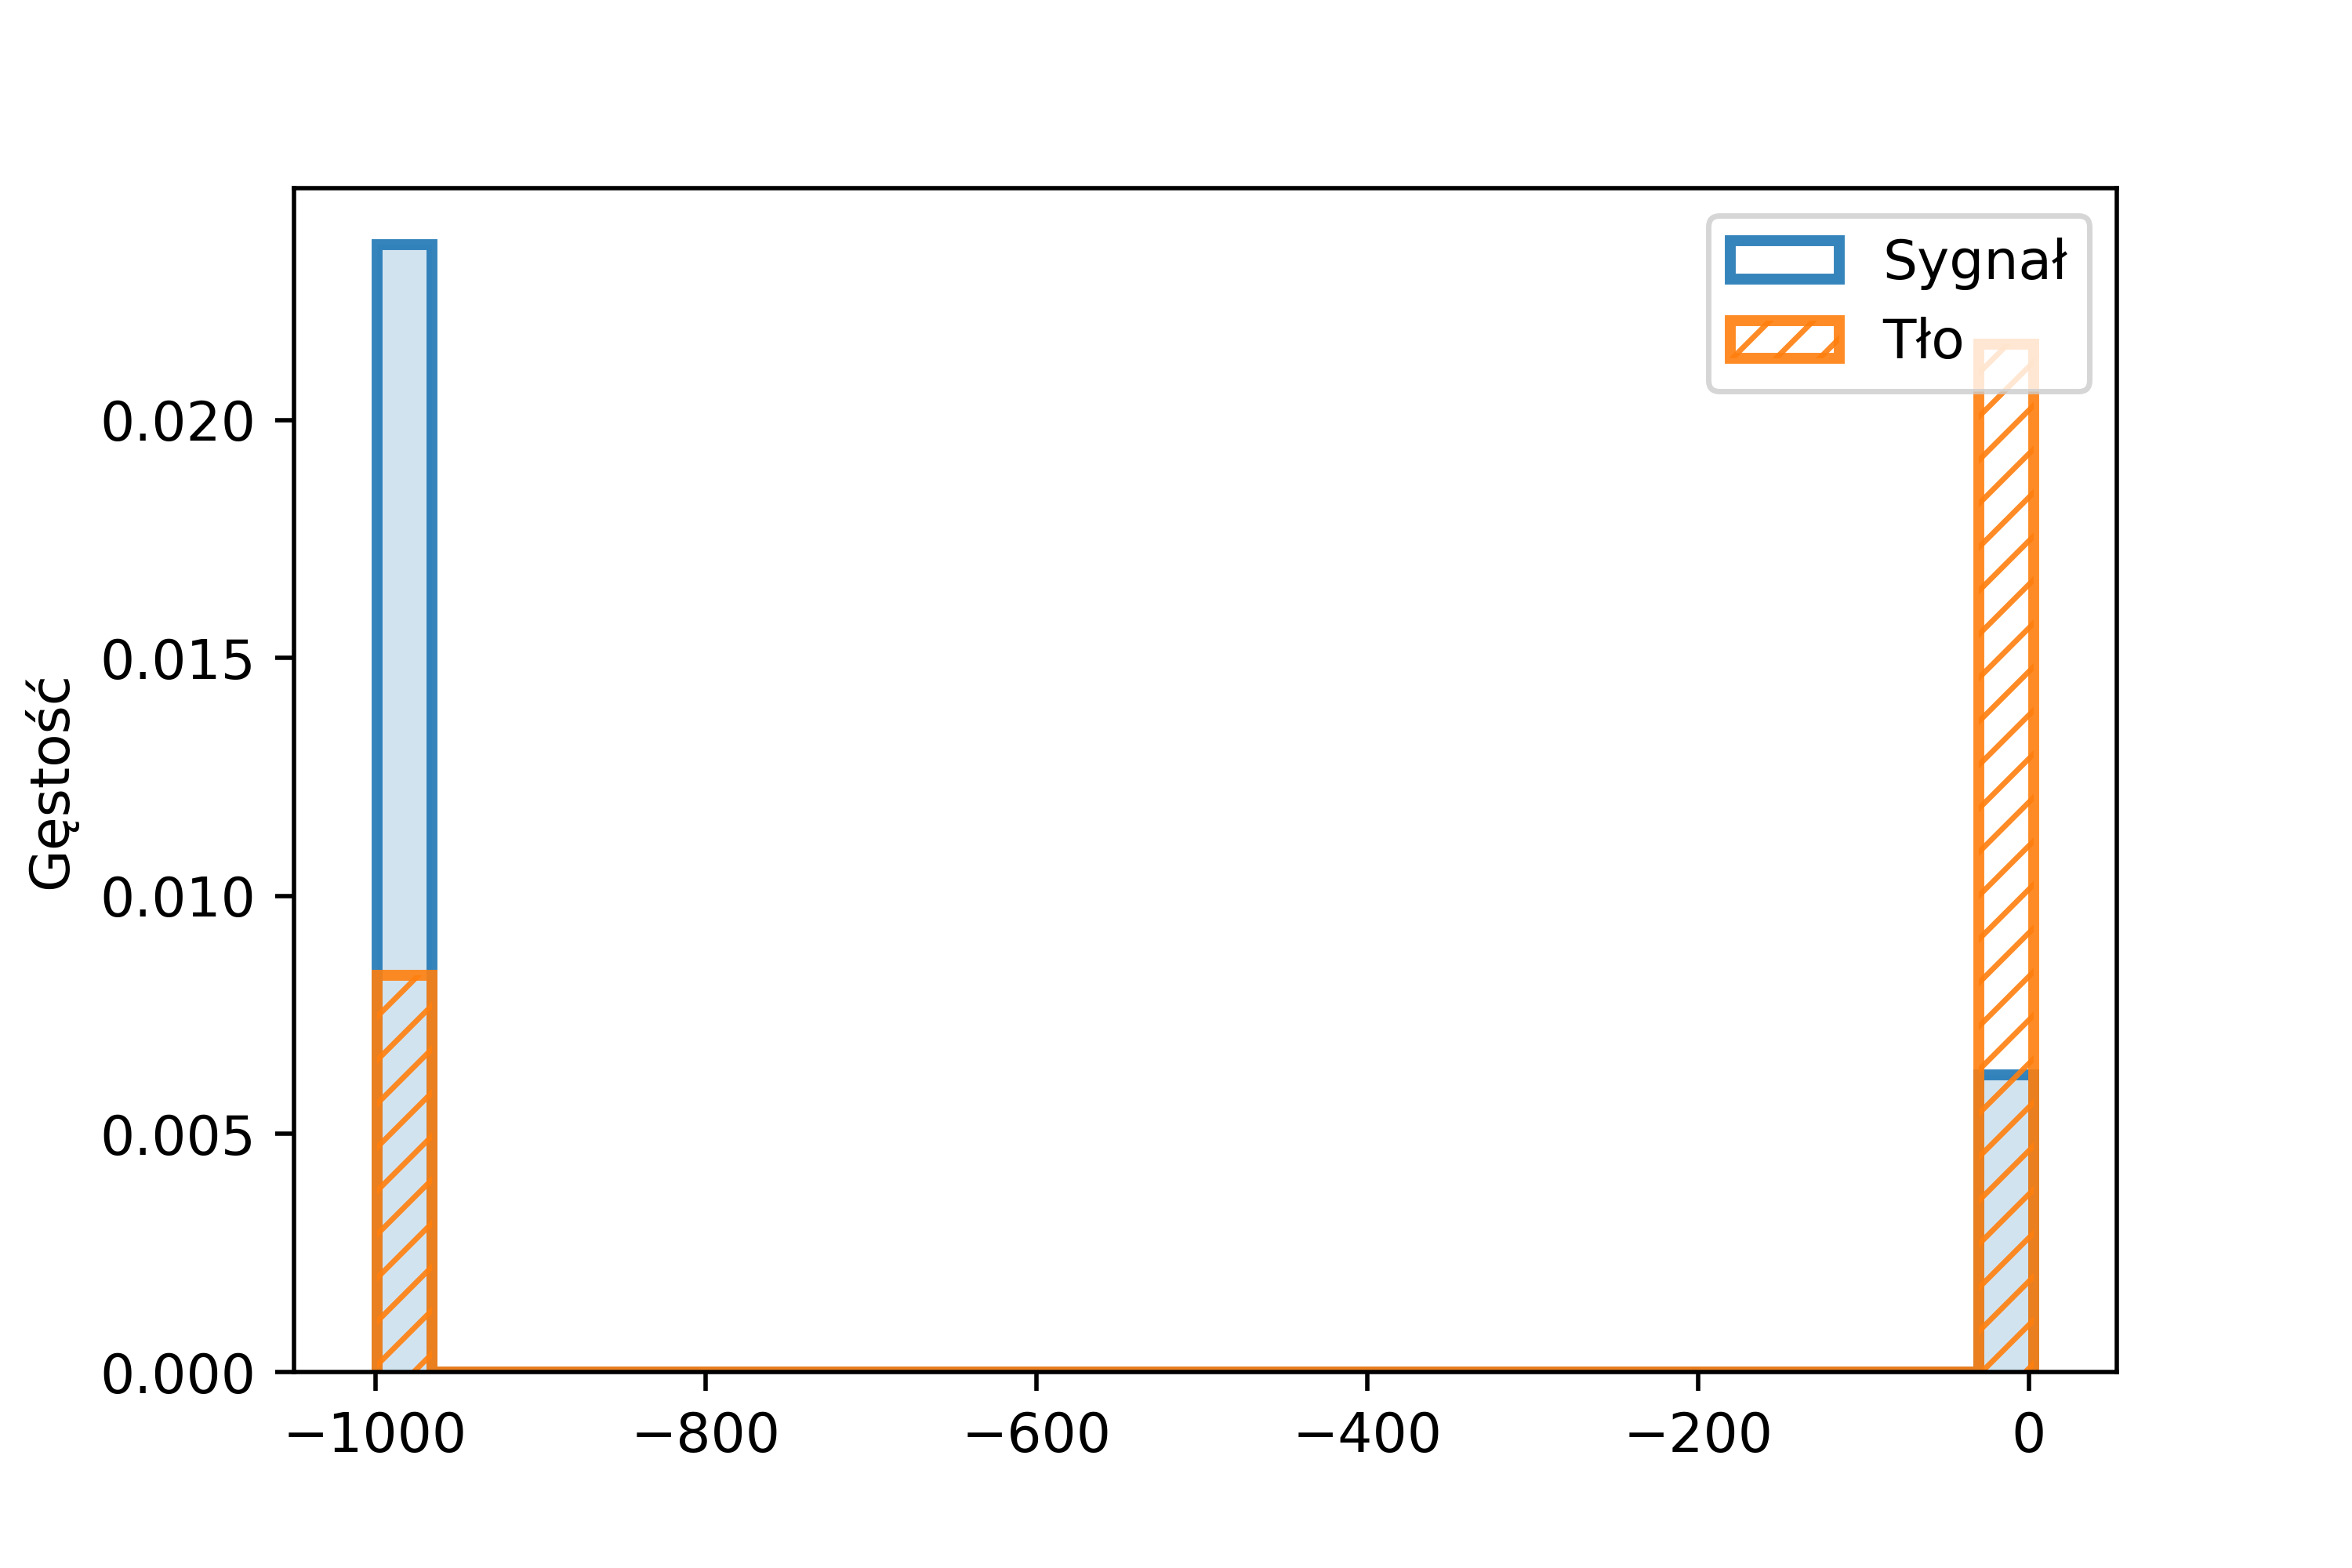
\includegraphics[width=1\textwidth]{difference_gjAngleDiff.png}
	\caption{gjAngleDiff}
	\end{subfigure}
	\begin{subfigure}{.5\textwidth}
	\centering
	\includegraphics[width=1\textwidth]{difference_nPhoton.png}
	\caption{nPhoton}
	\end{subfigure}
	\caption{Rozkłady przykładowych zmiennych dla sygnału i tła}
	\label{fig:diff}
	\end{figure}	

		
    \chapter{Architektura modeli}
	Aby dokonywać klasyfikacji sygnału zastosowano różne modele predykcyjne opierające się na metodach opisanych w rozdziale \ref{ch:wstep}. Modele zostały napisane w języku \textit{python} z wykorzystaniem bibliotek \textit{keras} oraz \textit{xgboost}. Kod jest dostępny w repozytorium: \url{https://github.com/byrolew/licencjat}.
	\section{Model oparty o same klasyfikatory}
	\label{sec:mod1}
	Prosty model, składający się z jednego neuronu, który przyjmuje jako zmienne objaśniające odpowiedzi wcześniej używanych klasyfikatorów (patrz rozdział \ref{ch:dane}). Jest to więc średnia ważona odpowiedzi klasyfikatorów, na którą nałożona jest funkcja sigmoid. Wielkość batcha została ustalona na 128, do optymalizacji został użyty algorytm \textit{Adam} ze stałą uczenia $\gamma = 10^{-3}$. Model uczony był przez cztery epoki. Później używana jest nazwa \textit{ensemble}.

	\section{Sieć neuronowa}
	\label{sec:mod2}
	Kolejny model był oparty o wszystkie zmienne objaśniające, jego architekturę przedstawiono na rysunku \ref{fig:nn1}. Składał się z sześciu warstw gęstych, o wielkości 32 neuronów każda. Jako funkcje aktywacji zastosowano funkcje ReLU. Warstwę wyjściową tworzy jeden neuron z sigmoidem jako funkcją aktywacji. Dzięki temu wyjściem sieci jest pojedyncza wartość z zakresu [0, 1]. Inne parametry zostały ustalone tak samo jak dla modelu w sekcji \ref{sec:mod1}. Ten model zwany jest później jako \textit{baseline}.
	
	\section{Poprawiona sieć neuronowa}
	Na podstawie optymalizacji hiperparametrów przy pomocy losowego przeszukiwania został wybrany najlepszy model oparty o gęste sieci neuronowe. Optymalizowano parametry takie jak: wielkość batcha, stała uczenia, wielkość i liczba warstw ukrytych, funkcja aktywacji, liczba epok, występowanie warstwy \textit{batch normalization} i występowanie harmonogramu stałej uczenia. Otrzymana architektura znajduje się na rysunku \ref{fig:nn2}. 
	
	Wybrany model ma dwie warstwy gęste po 256 neuronów każda, zatem widać że model jest płytszy i szerszy niż opisany w sekcji \ref{sec:mod2}. Jako funkcja aktywacji jest tutaj użyty sigmoid, a dodatkowo zastosowana jest warstwa \textit{batch normalization}. Użyta wielkość batcha to 256, do optymalizacji  zastosowano algorytm \textit{Adam} ze stałą uczenia $\gamma = 5\cdot 10^{-4}$ oraz harmonogram zmniejszający stałą uczenia $\gamma$ na wypłaszczeniu funkcji straty przez czynnik 0.2 do minimalnej wartości $\gamma = 10^{-5}$. Model był uczony przez sześć epok. Ten model zwany jest później jako \textit{best-nn}.

	\begin{figure}[H]
	\centering
	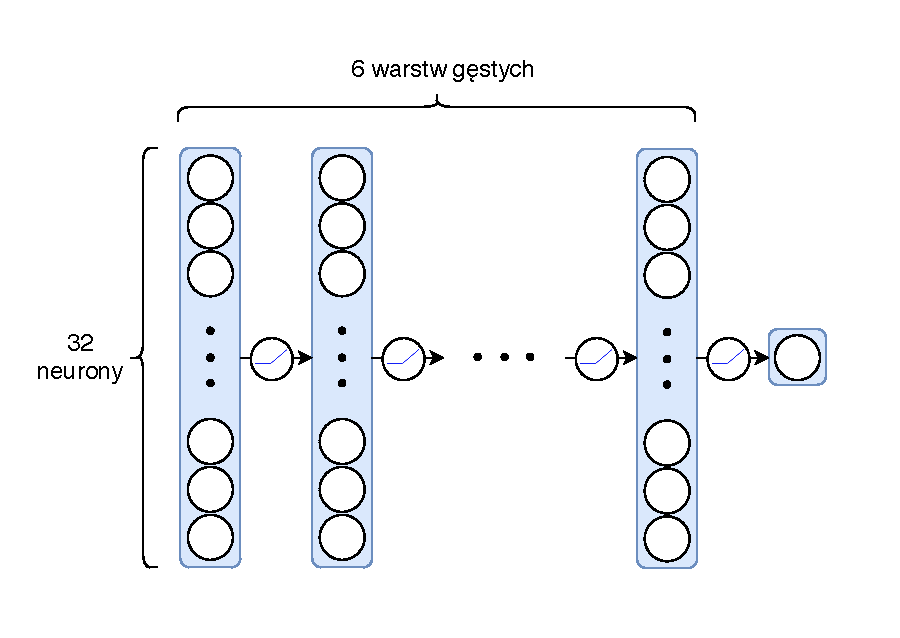
\includegraphics[width=0.75\textwidth]{neural_net.pdf}
	\caption{Bazowa sieć neuronowa (\textit{baseline}). Składa się z 6 ukrytych warstw gęstych po 32 neurony. Jako funkcji aktywacji użyto ReLU.}
	\label{fig:nn1}
	\end{figure}
	
	\begin{figure}[H]
	\centering
	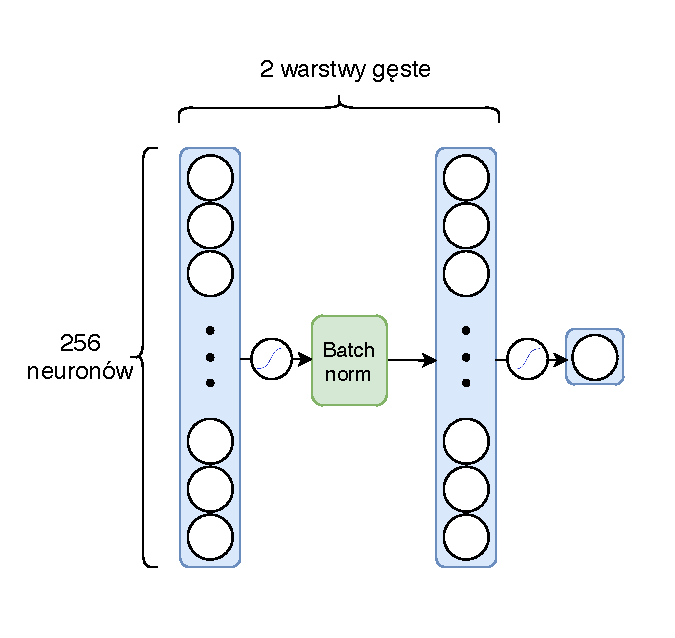
\includegraphics[width=0.65\textwidth]{best_neural_net.pdf}
	\caption{Zoptymalizowana sieć neuronowa (\textit{best-nn}). Składa się z dwóch ukrytych warstw gęstych oraz warstwy \textit{batch normalization}. Jako funkcji aktywacji użyto sigmoida.}
	\label{fig:nn2}
	\end{figure}

	
	\section{XGBoost}
	Model oparty na XGBoost składał się ze 100 drzew decyzyjnych o maksymalnej głębokości 3. Wykorzystano stałą uczenia $\gamma = 10^{-1}$, funkcją kosztu była binarna entropia krzyżowa (tak samo jak w przypadku sieci neuronowych). Schematyczny rysunek architektury znajduje się na rysunku \ref{fig:xgb}.
	
	\begin{figure}[H]
	\centering
	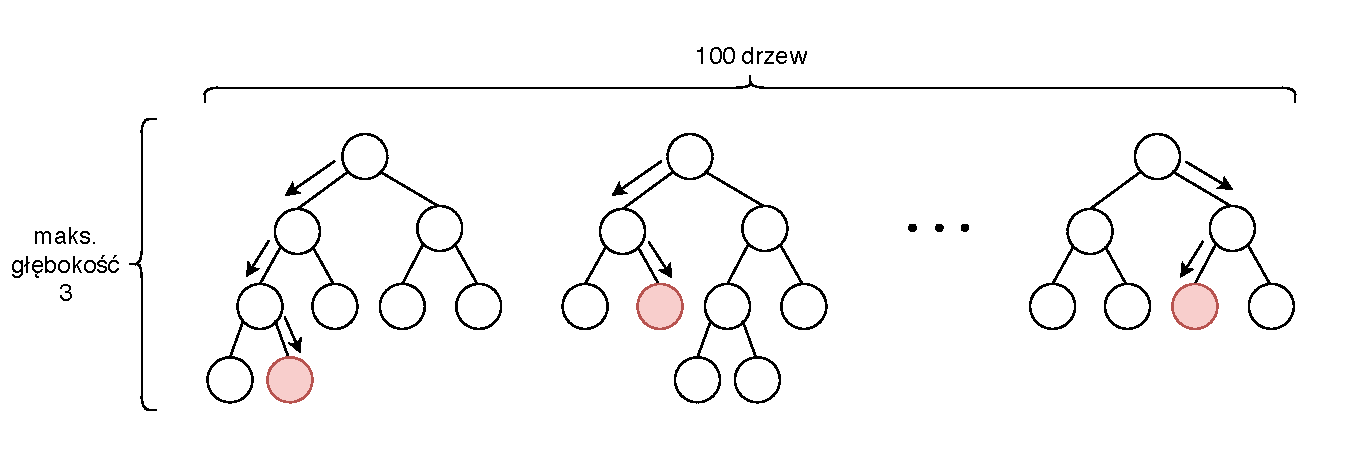
\includegraphics[width=1.0\textwidth]{xgb.pdf}
	\caption{Architektura modelu typu XGBoost opartego na drzewach decyzyjnych. Tutaj użyto modelu zawierającego 100 drzew o maksymalnej głębokości 3 (nie licząc korzenia).}
	\label{fig:xgb}
	\end{figure}
    
    \chapter{Wyniki}
    Każdy model trenowany był w dwóch trybach. Pierwszy z nich korzystał ze wszystkich zmiennych objaśniających, drugi zaś pomijał odpowiedzi klasyfikatorów. Dzięki temu można porównać wyniki z wcześniej używanymi modelami. Po dokonaniu analizy istotności zmiennych metodą permutacyjną zauważono, że zmienna byCombinedIsolationDeltaBetaCorrRaw3Hits (patrz rozdział \ref{ch:dane}) jest najbardziej istotna dla wszystkich modeli. Jako, że rozkład tej zmiennej różni się na danych symulacyjnych oraz eksperymentalnych, postanowiono wytrenować również modele bez tej zmiennej.
    
	W tabeli \ref{tab:wyniki} znajdują się wyniki ROC AUC dla wszystkich modeli. Dla porównania zamieszczono wynik najlepszego z wcześniejszych klasyfikatorów, którym okazał się deepTau2017v1tauVSjet (później nazywany \textit{deepTau}). 
	
	Można zauważyć, że model oparty o XGBoost osiąga najwyższą skuteczność spośród zaproponowanych oraz wcześniej używanych modeli. W szczególności przy treningu na danych z wyłączeniem klasyfikatorów zarówno \textit{best-nn} jak i \textit{XGBoost} osiągnęły lepsze wyniki niż \textit{deepTau}. Widać również, że wyrzucenie głównej zmiennej nie pogarsza znacząco skuteczności modeli, a może skutkować lepszymi wynikami na danych eksperymentalnych. Ponadto, model oparty o same klasyfikatory osiąga lepszy wynik niż każdy klasyfikator osobno.
	
	
	\begin{table}[H]
	\centering
	\caption{Wartość ROC AUC dla wszystkich modeli na zbiorze testowym, pogrubioną czcionką zaznaczono najlepszy wynik.}
	\label{tab:wyniki}
	\begin{tabular}{lrrrrr}
	\toprule
	Tryb & \textit{baseline} & \textit{best-nn} & \textit{XGBoost} & \textit{deepTau} & \textit{ensemble} \\
	\midrule
	Pełne dane & .9948 & .9979 & \textbf{.9985} & $-$ & $-$ \\
	Bez klas. & .9940 & .9949 & \textbf{.9956} & .9945 & $-$  \\
	Bez najlepszej & .9977 & .9972 & \textbf{.9985} & $-$ & $-$ \\
	Same klas. & $-$ & $-$ & $-$ & $-$ & .9956 \\
	\bottomrule
	\end{tabular}
	\end{table}
	
	Na rysunku \ref{fig:dist} przestawiono rozkłady odpowiedzi modeli dla sygnału oraz tła. Widać, że rozkłady wyglądają podobnie dla wszystkich modeli, maksimum dla sygnału przypada dla odpowiedzi modelu równej 1, a dla tła dla odpowiedzi równej 0. Można zauważyć, że histogram gęstości odpowiedzi modelu osiąga mniejsze wartości dla odpowiedzi nieprawidłowych na obserwacjach oznaczonych w danych jako tło niż na tych oznaczonych w danych jako sygnał. Oznacza to, że model jest bardziej \textit{pewny} swoich odpowiedzi dla tła niż dla sygnału. Dodatkowo dla modeli \textit{ensemble} oraz \textit{baseline} w rozkładzie odpowiedzi dla sygnału widoczna jest górka w okolicy 0. Oznacza to, że dla części obserwacji oznaczonych w danych jako sygnał, model jest pewny, że jest to tło, co skutkuje niewykryciem taonu.

	\begin{figure}[H]
	\begin{subfigure}{.5\textwidth}
	\centering
	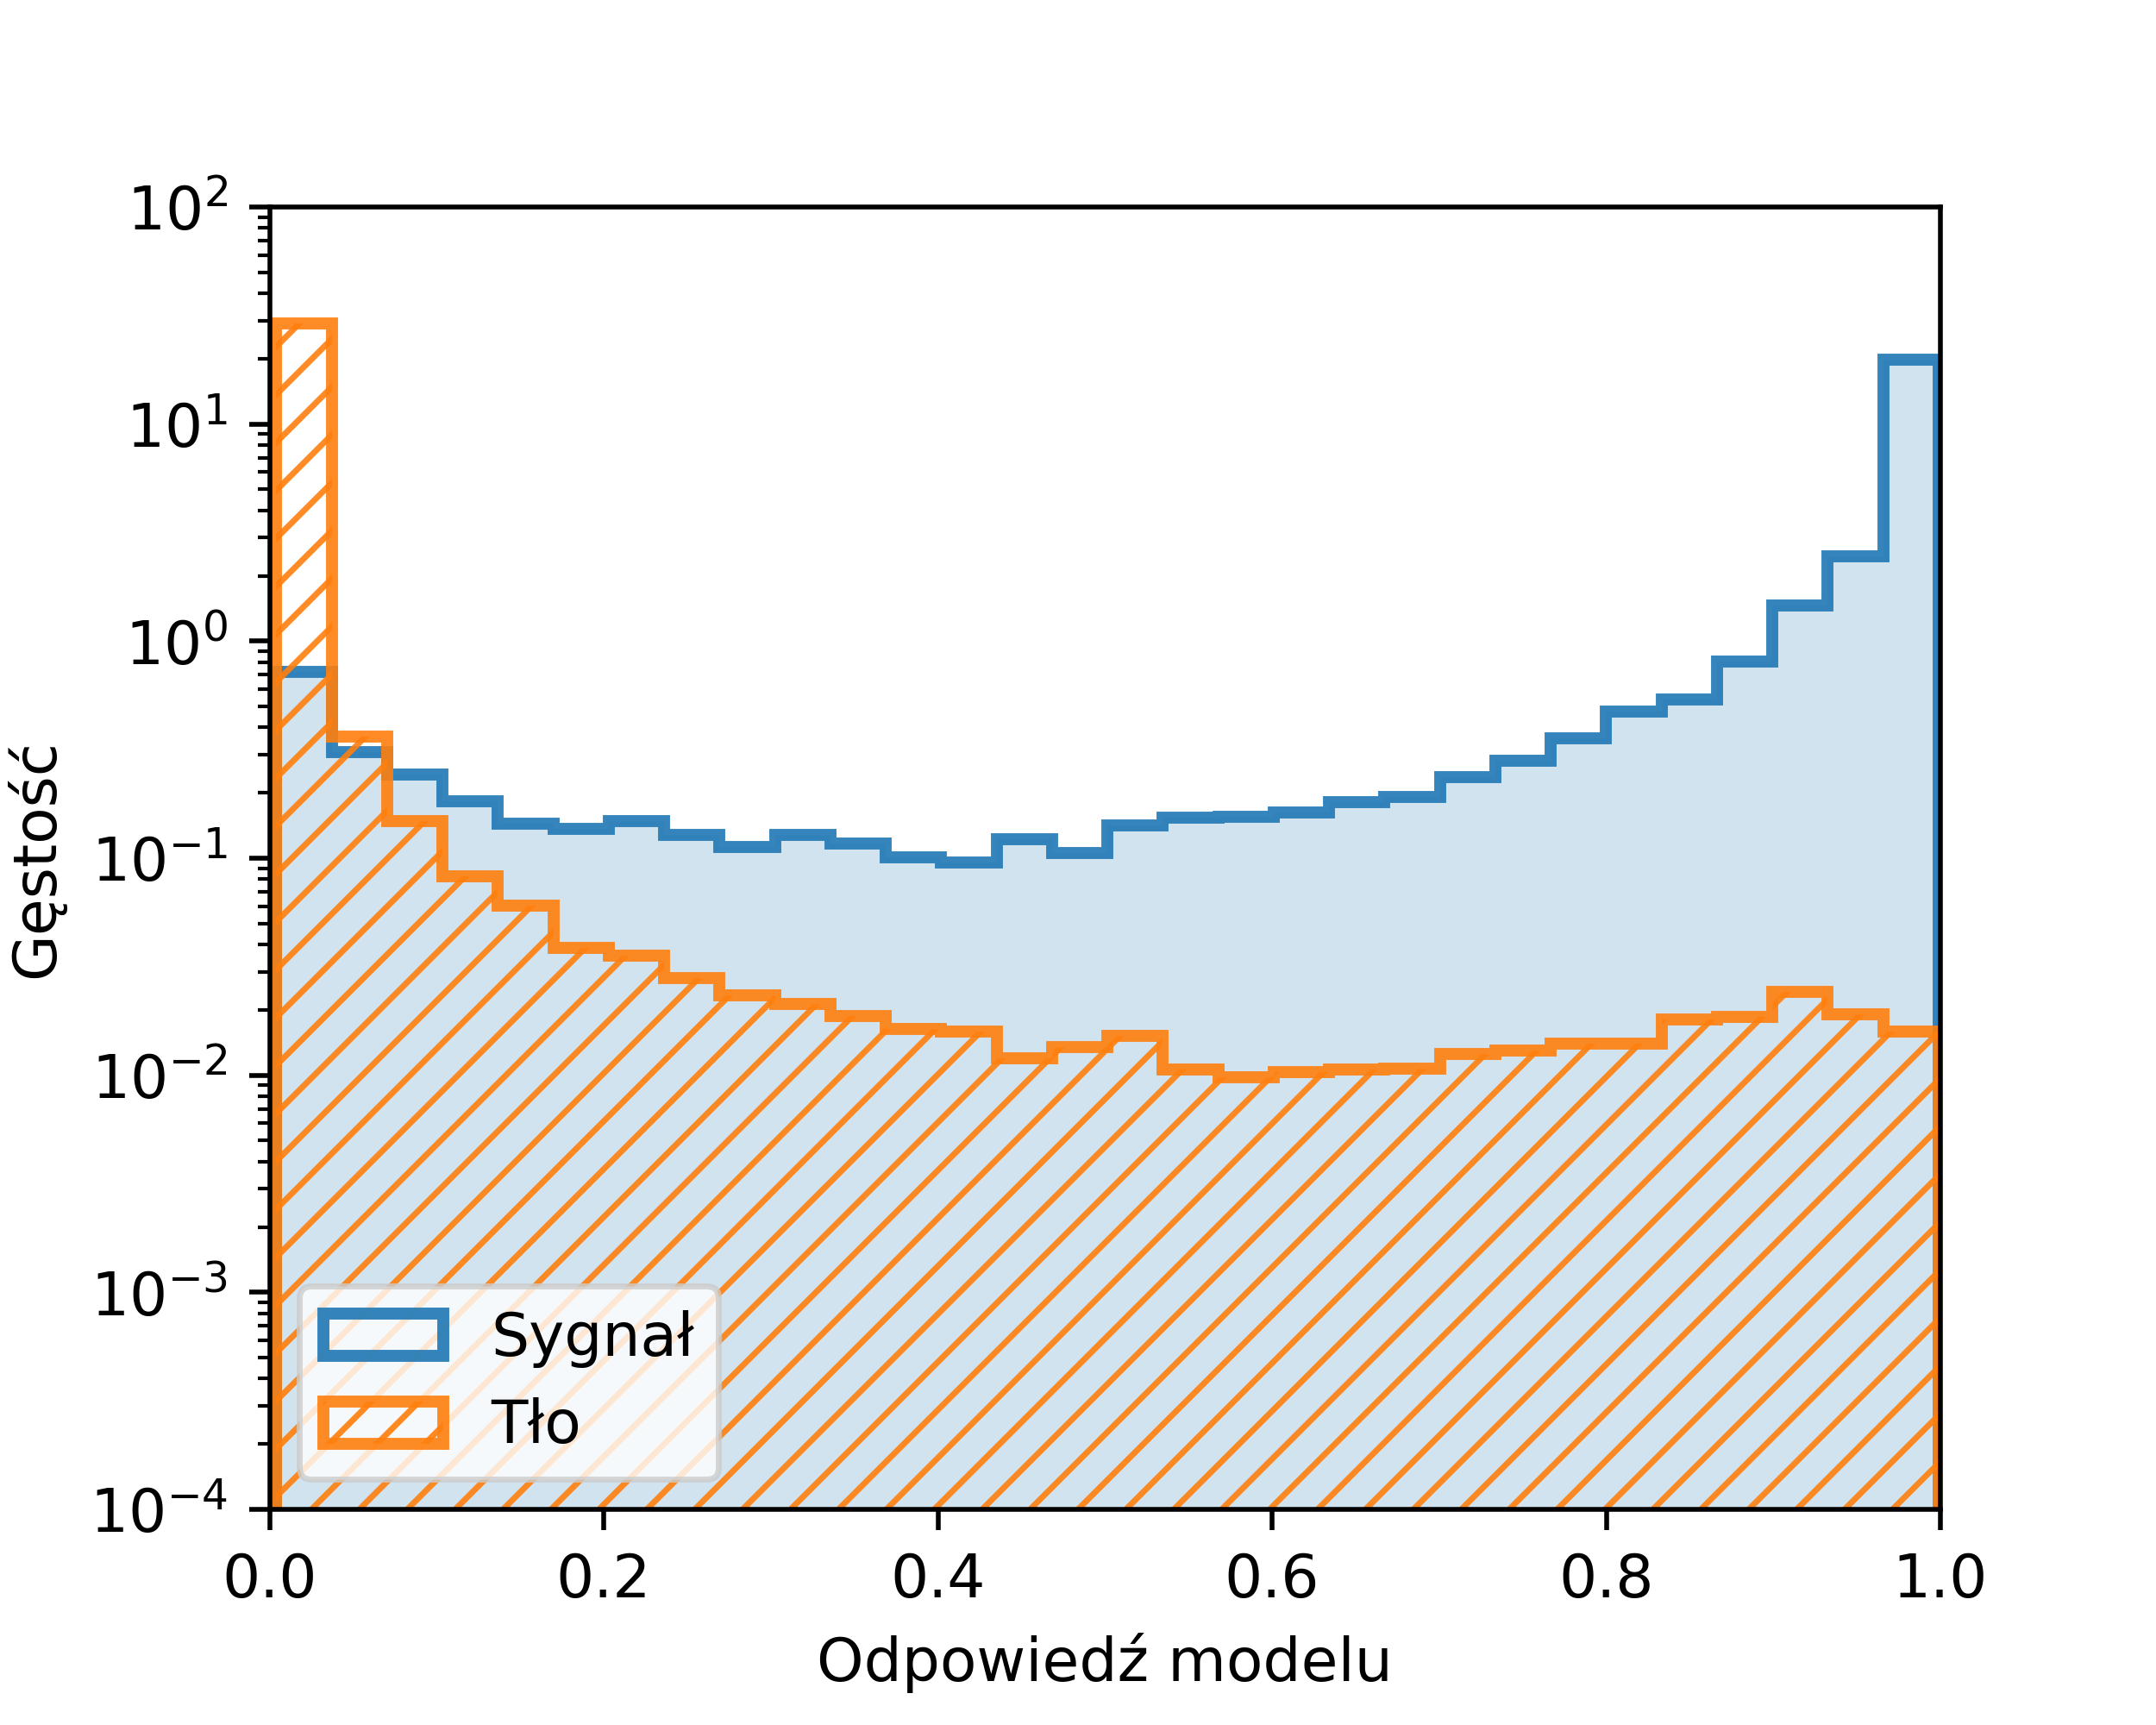
\includegraphics[width=1\textwidth]{density_ensemble.png}
	\caption{\textit{ensemble}}
	\end{subfigure}
	\begin{subfigure}{.5\textwidth}
	\centering
	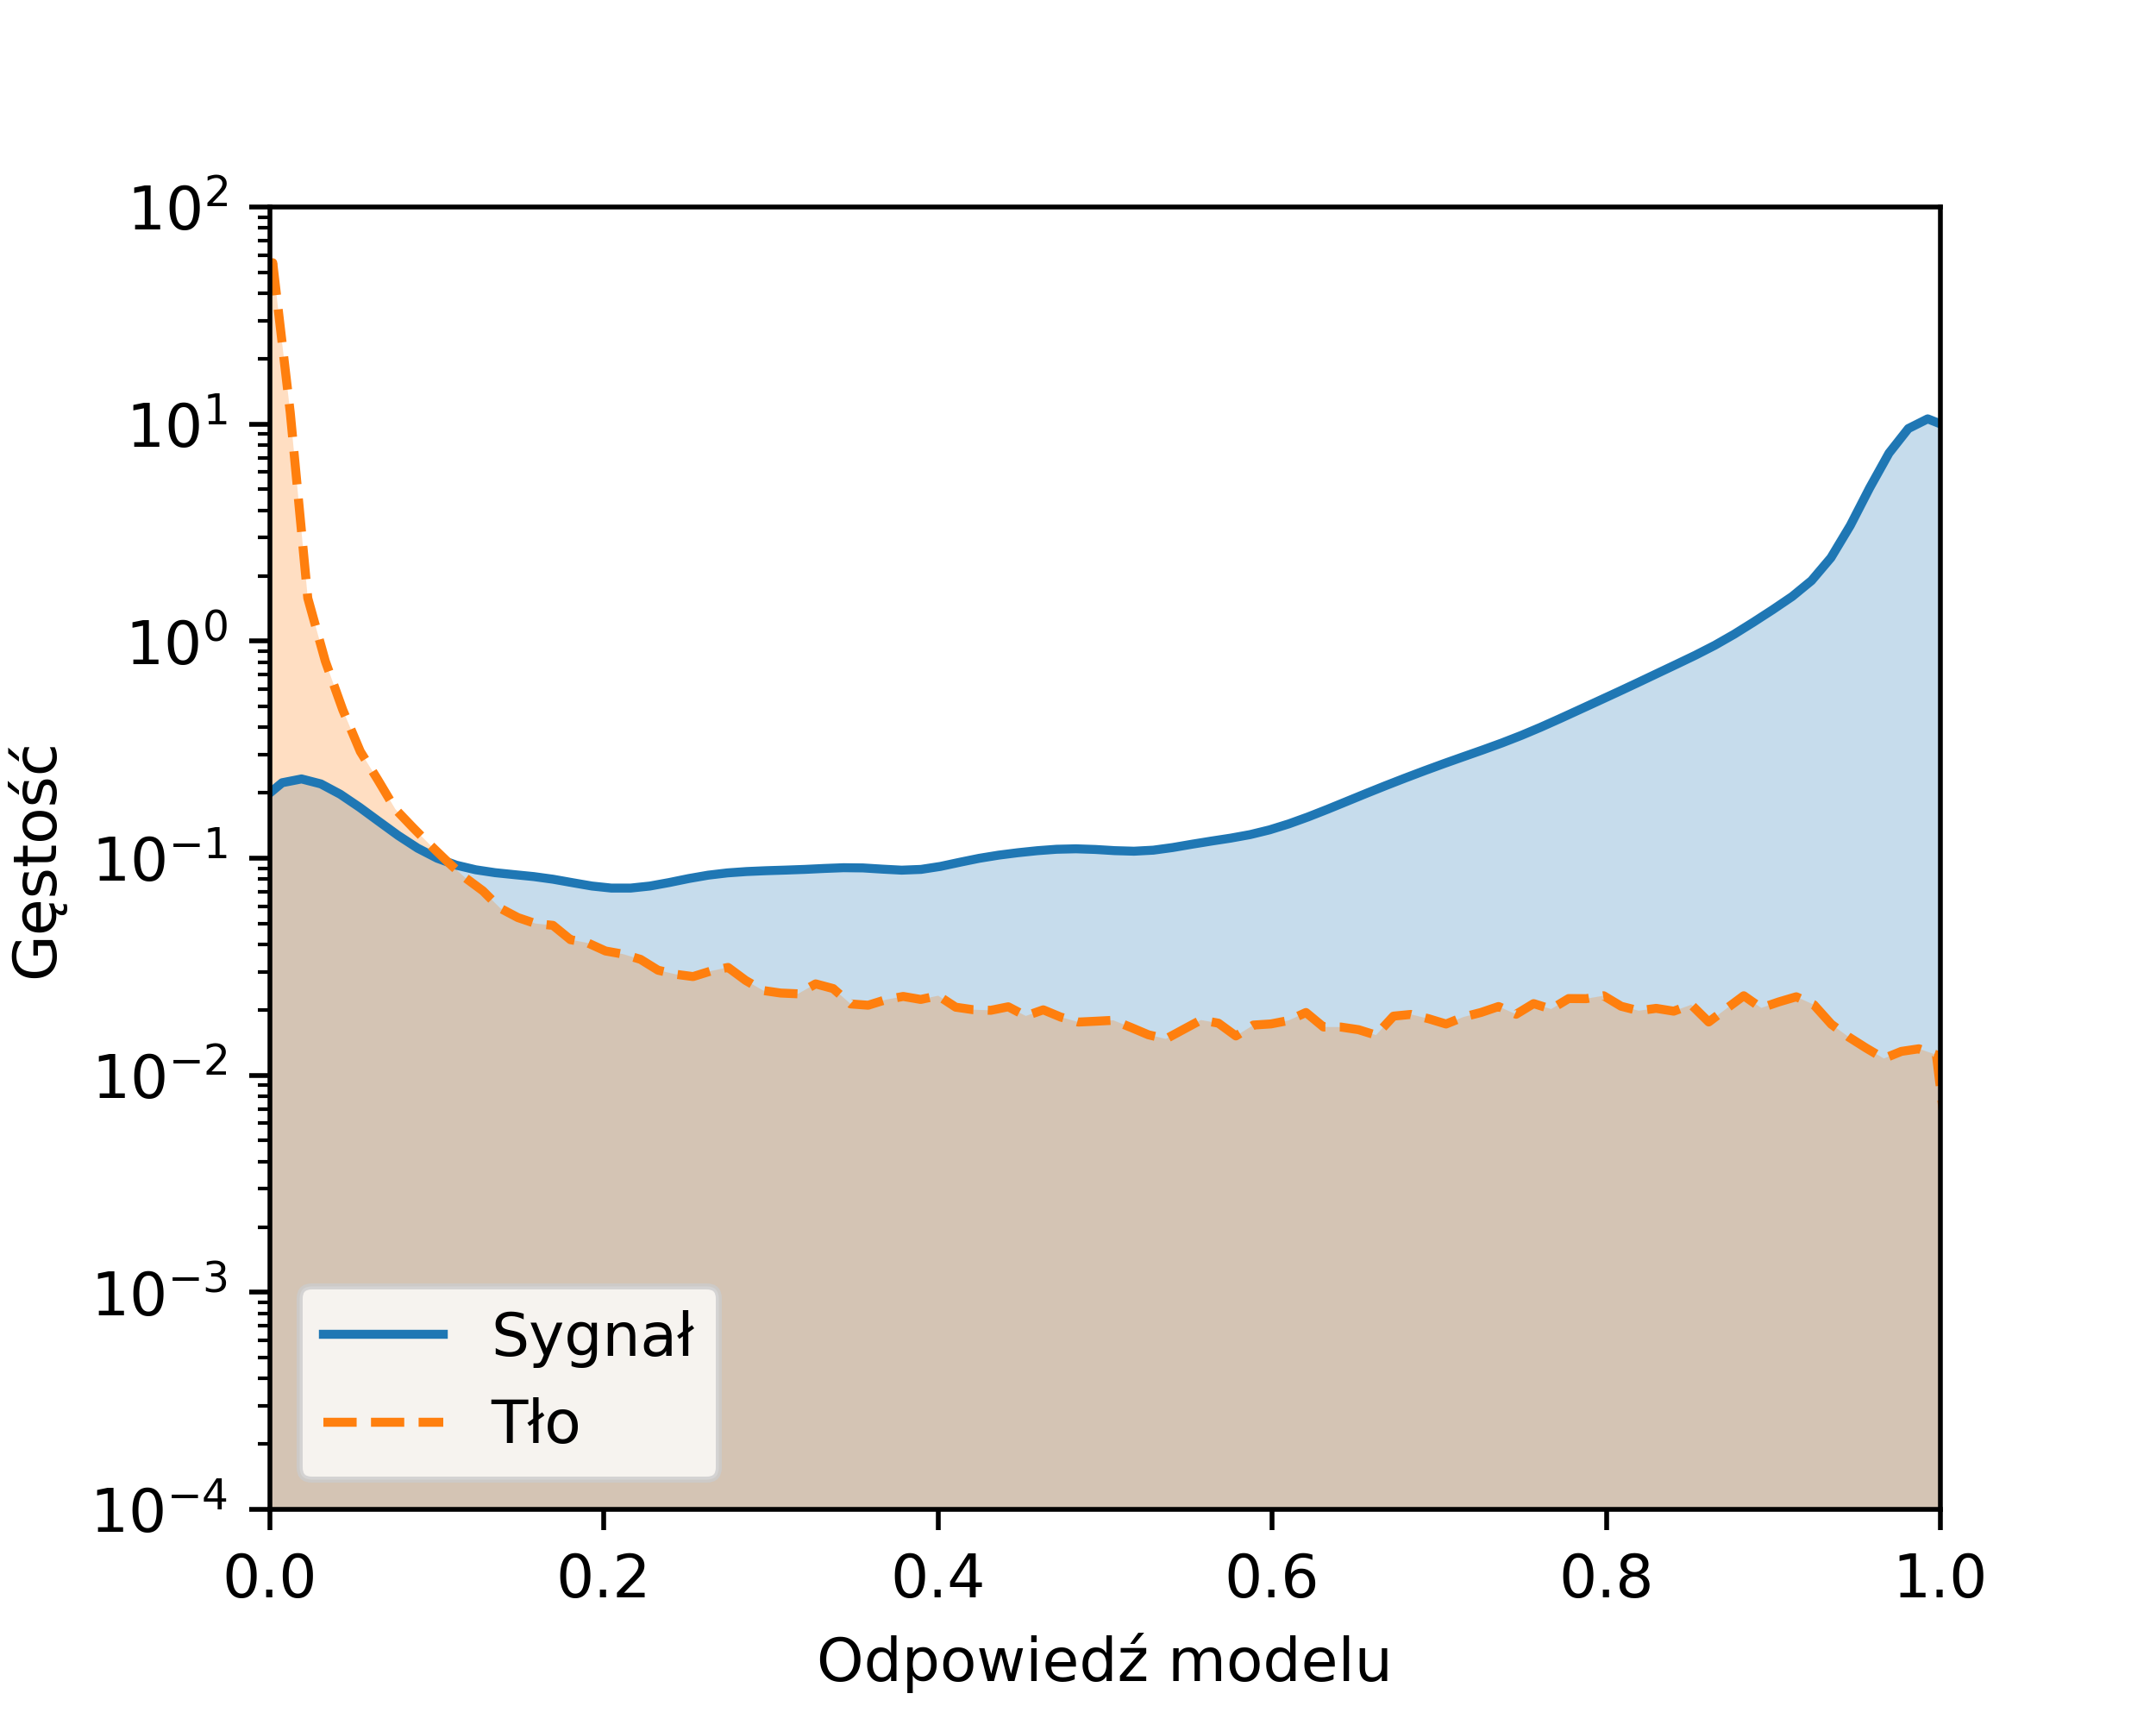
\includegraphics[width=1\textwidth]{density_baseline.png}
	\caption{\textit{baseline}}
	\end{subfigure}
	\begin{subfigure}{.5\textwidth}
	\centering
	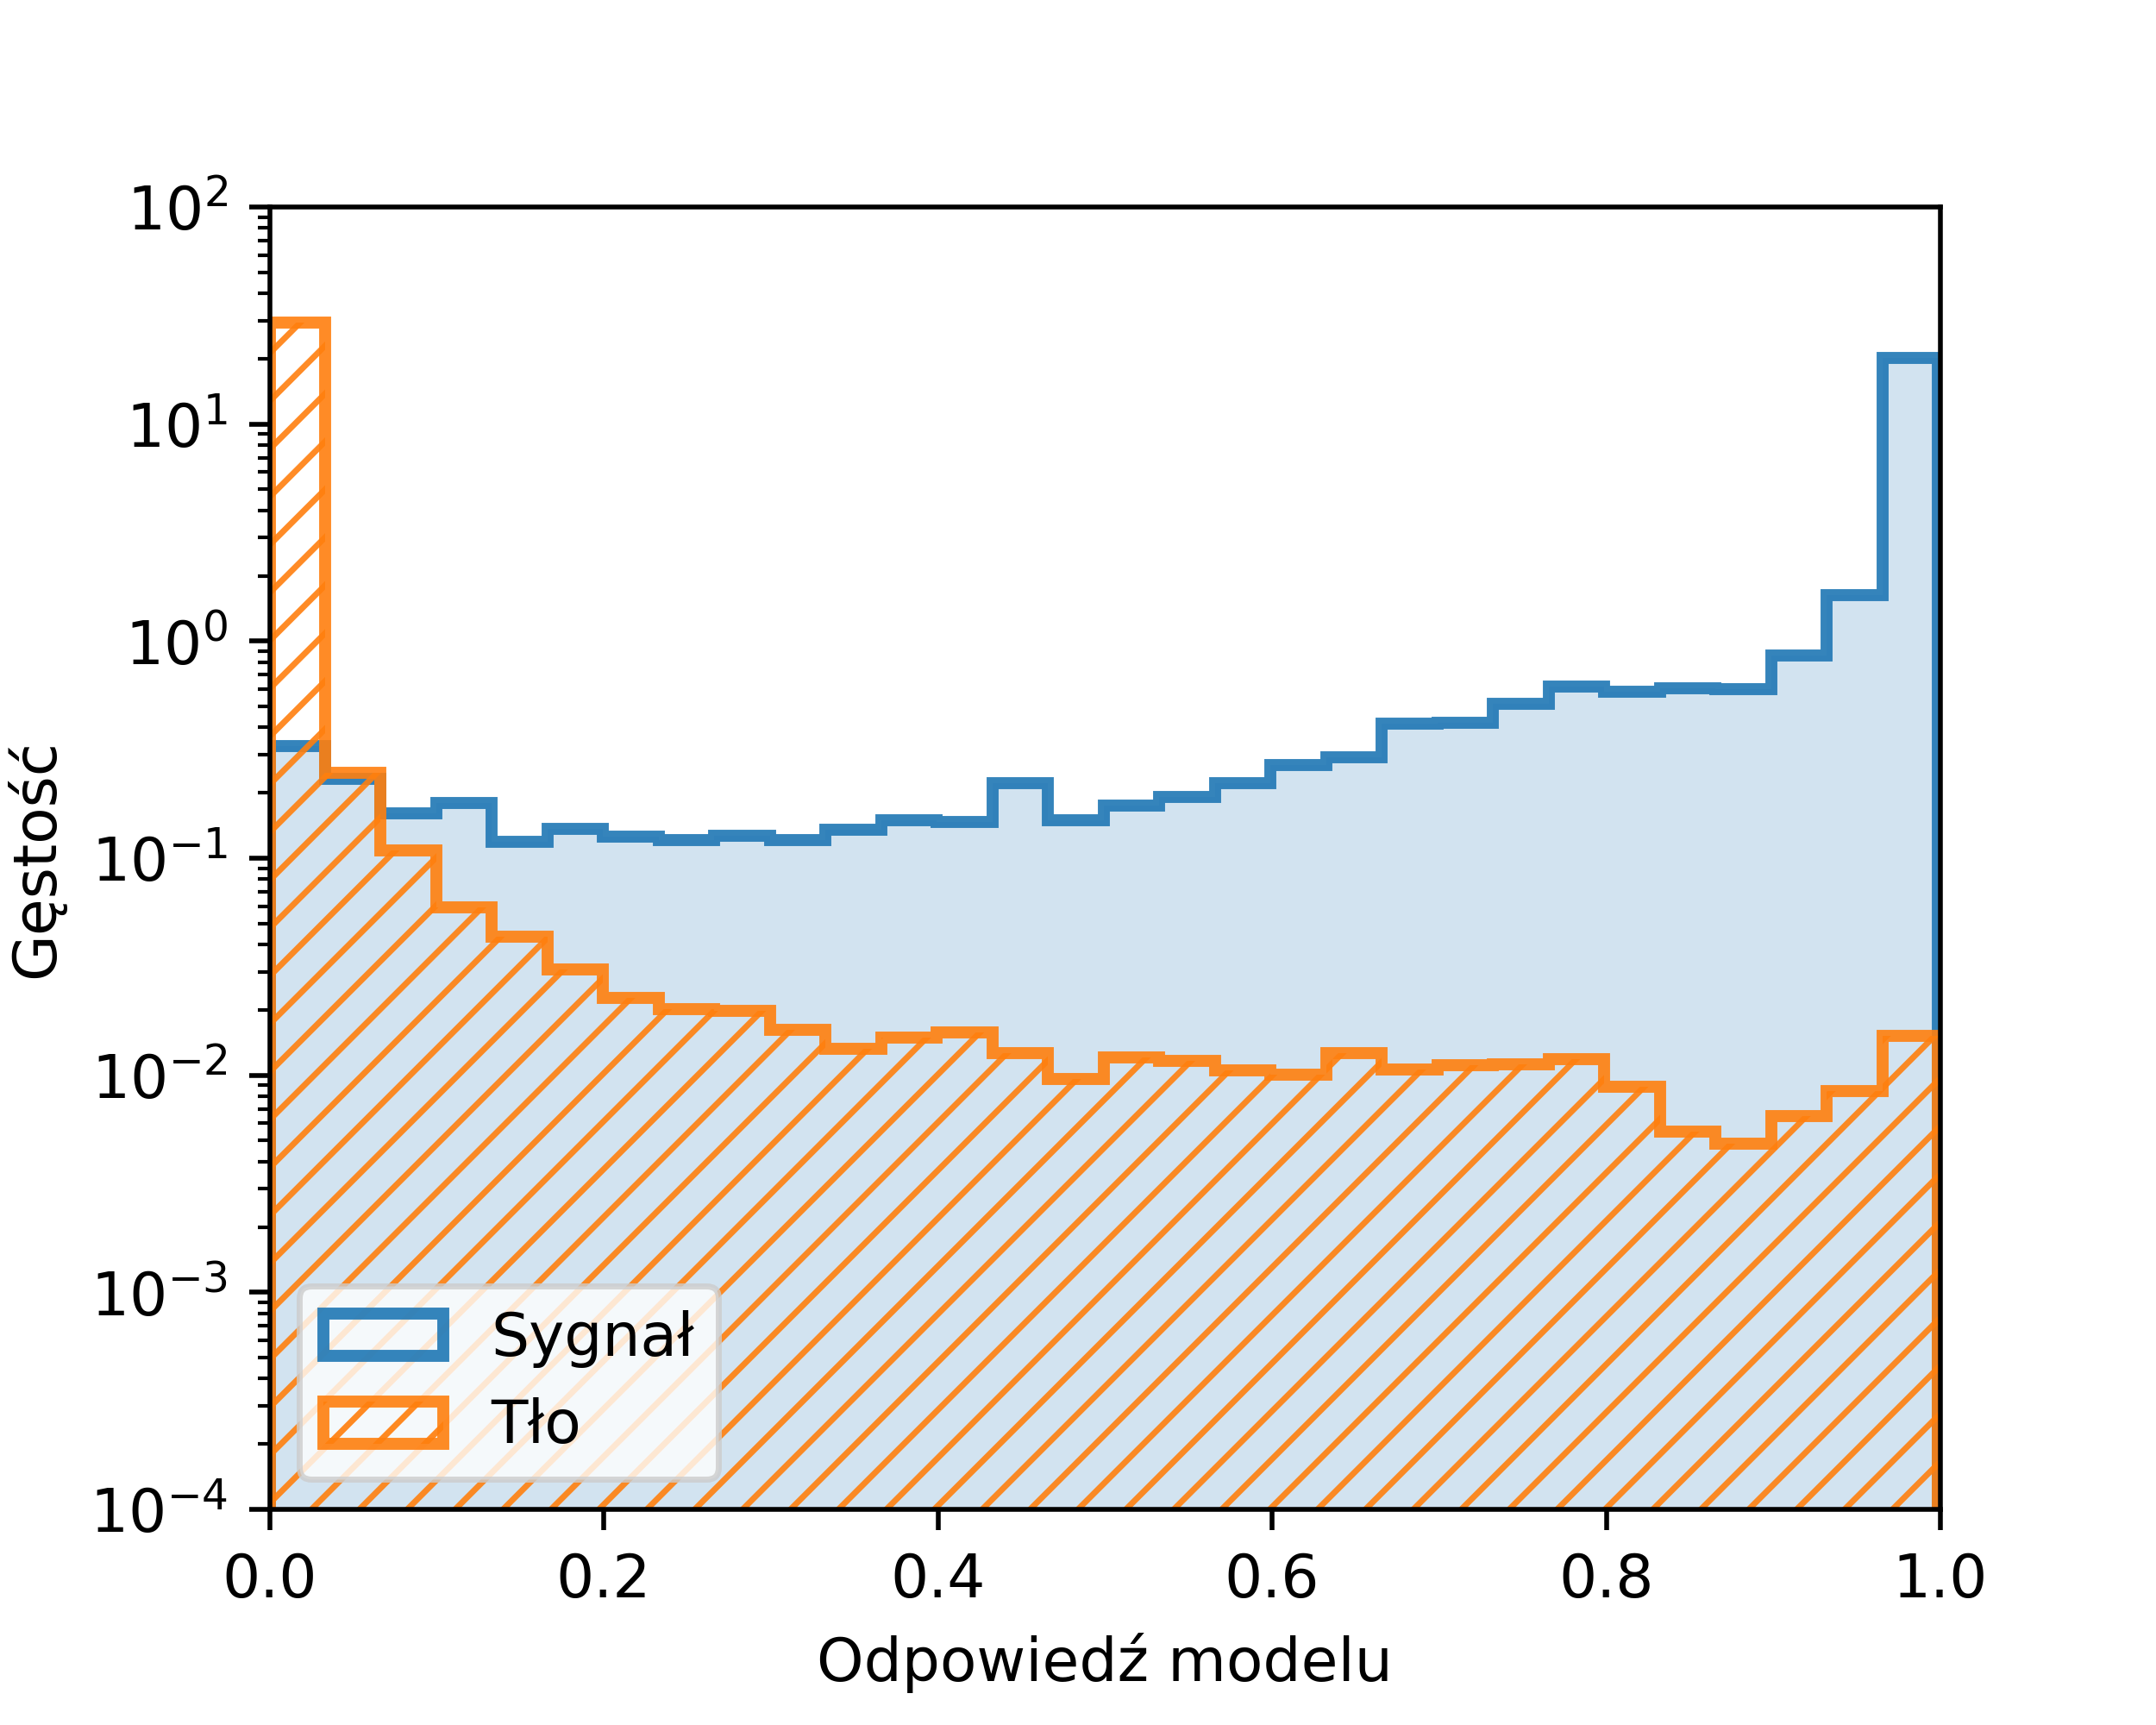
\includegraphics[width=1\textwidth]{density_best-nn.png}
	\caption{\textit{best-nn}}
	\end{subfigure}
	\begin{subfigure}{.5\textwidth}
	\centering
	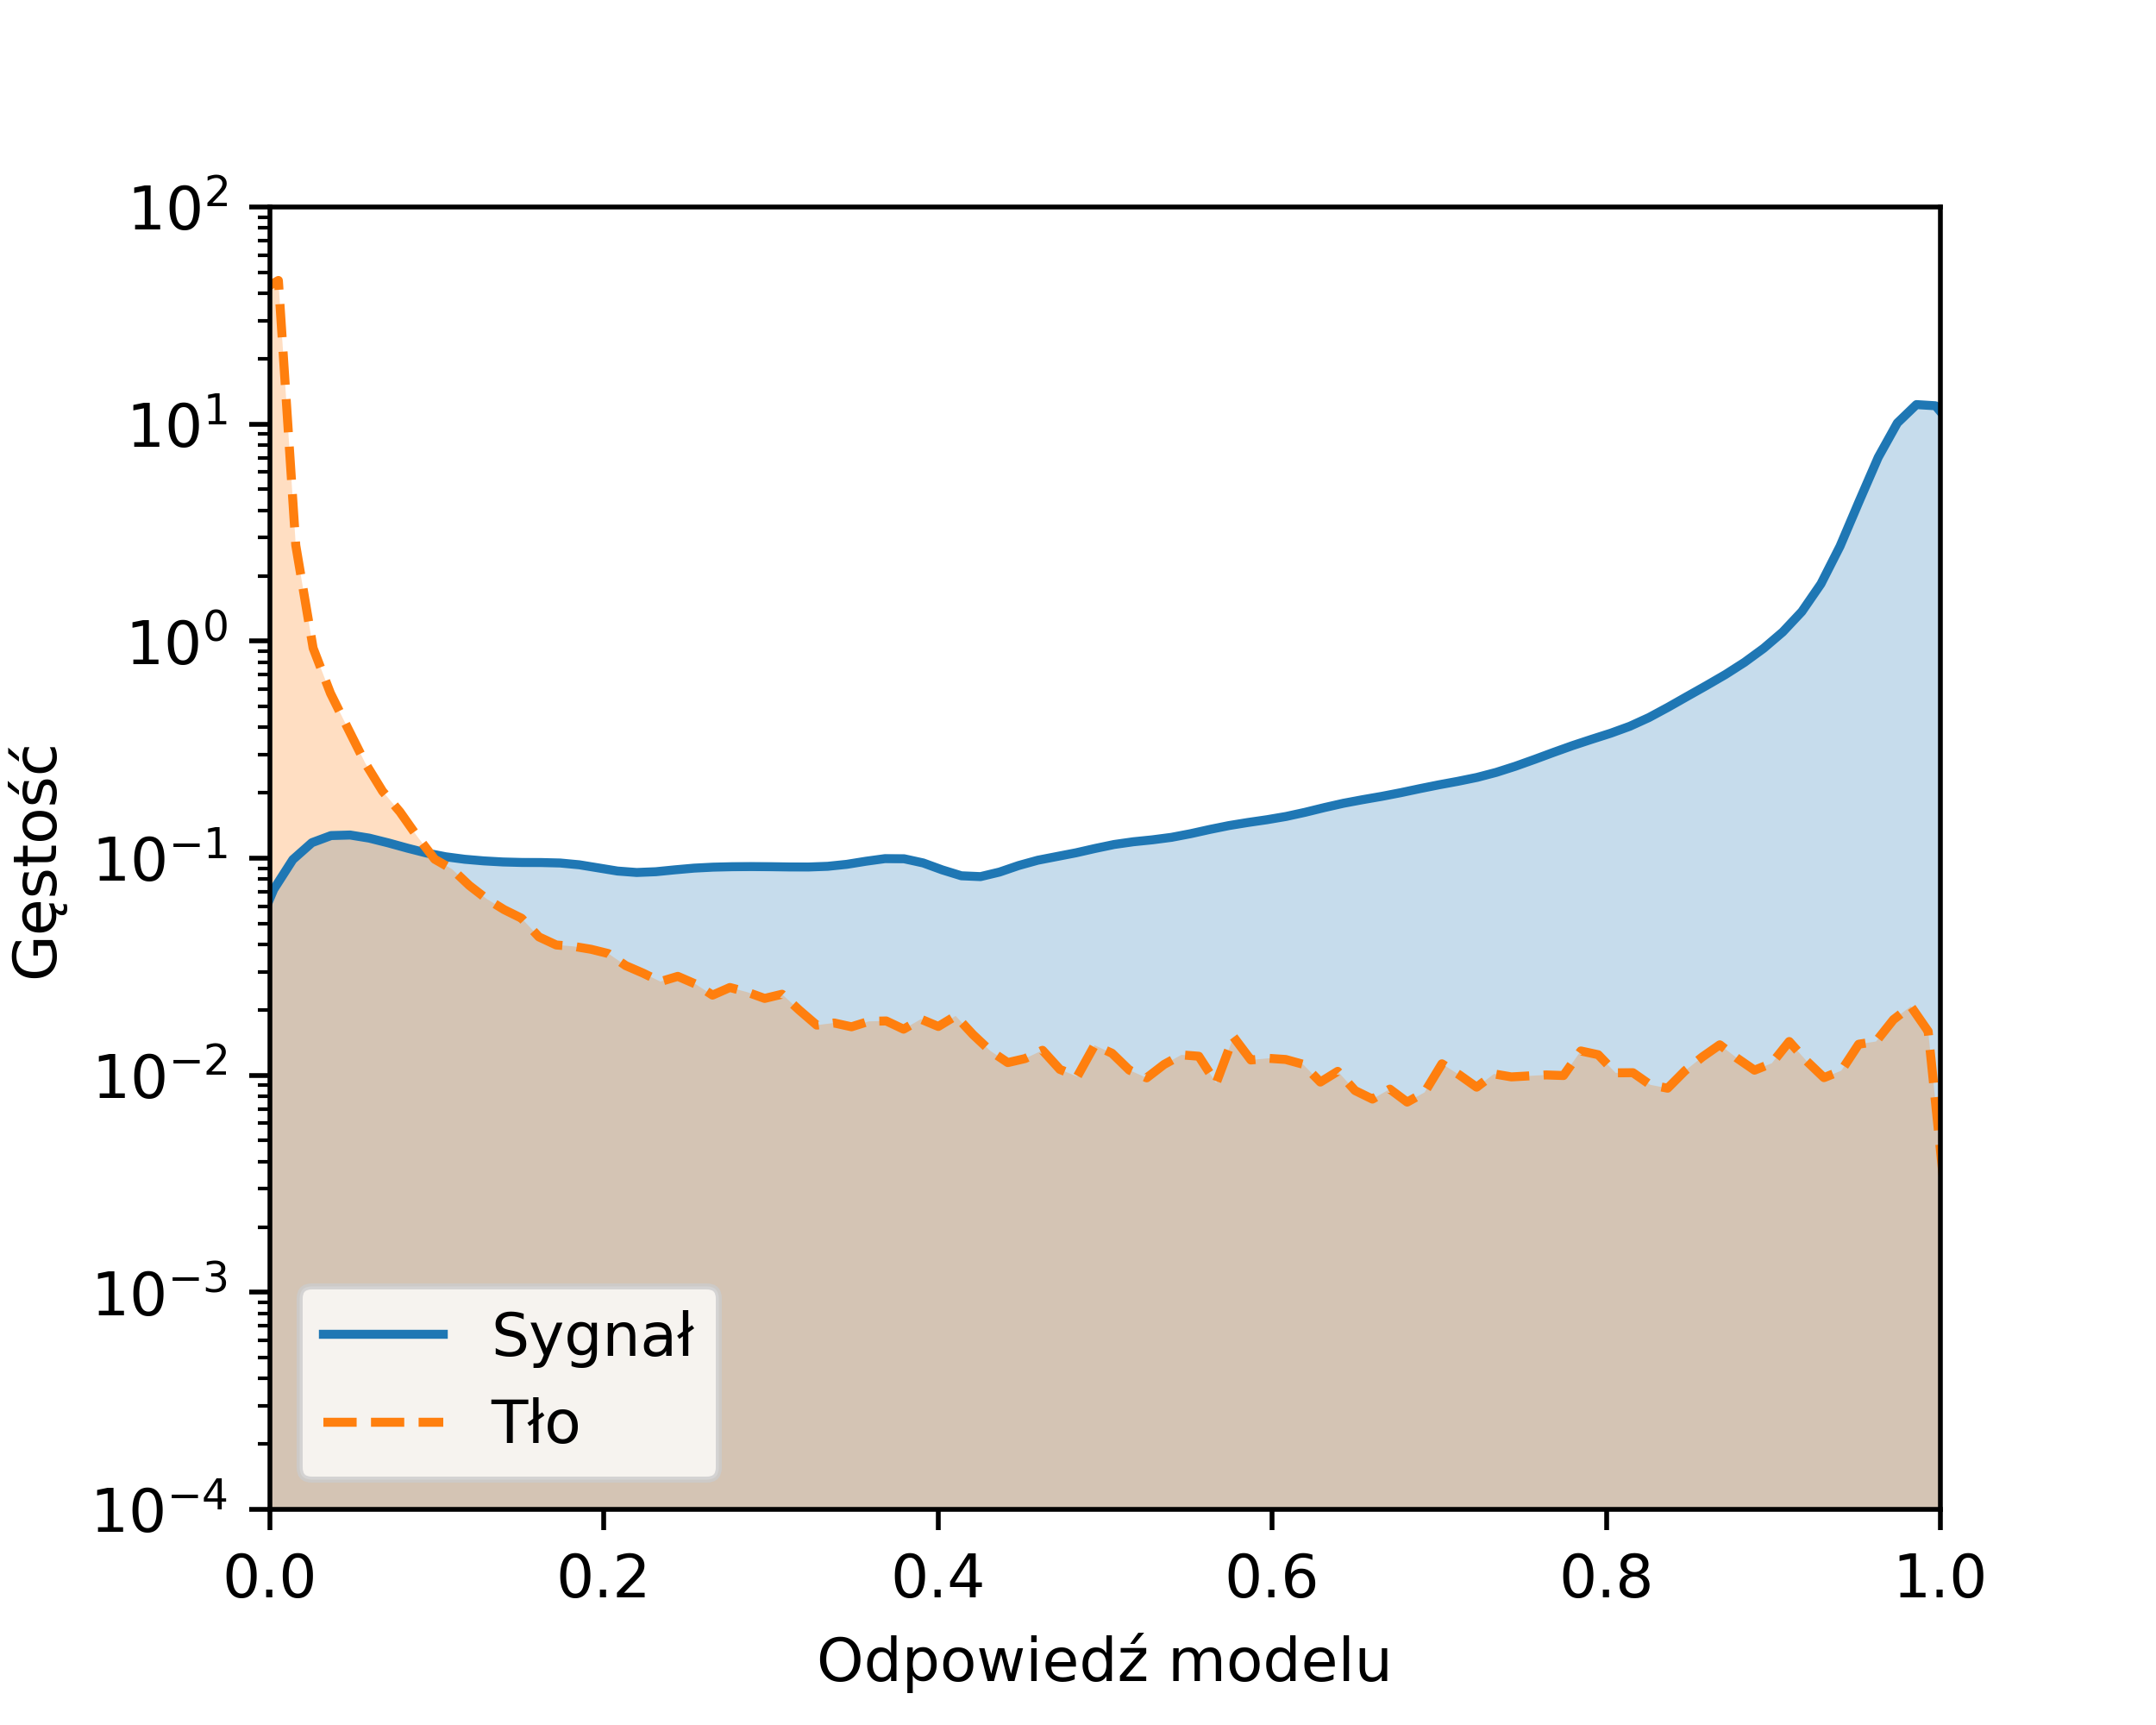
\includegraphics[width=1\textwidth]{density_XGBoost.png}
	\caption{\textit{XGBoost}}
	\end{subfigure}
	\begin{subfigure}{.5\textwidth}
	\centering
	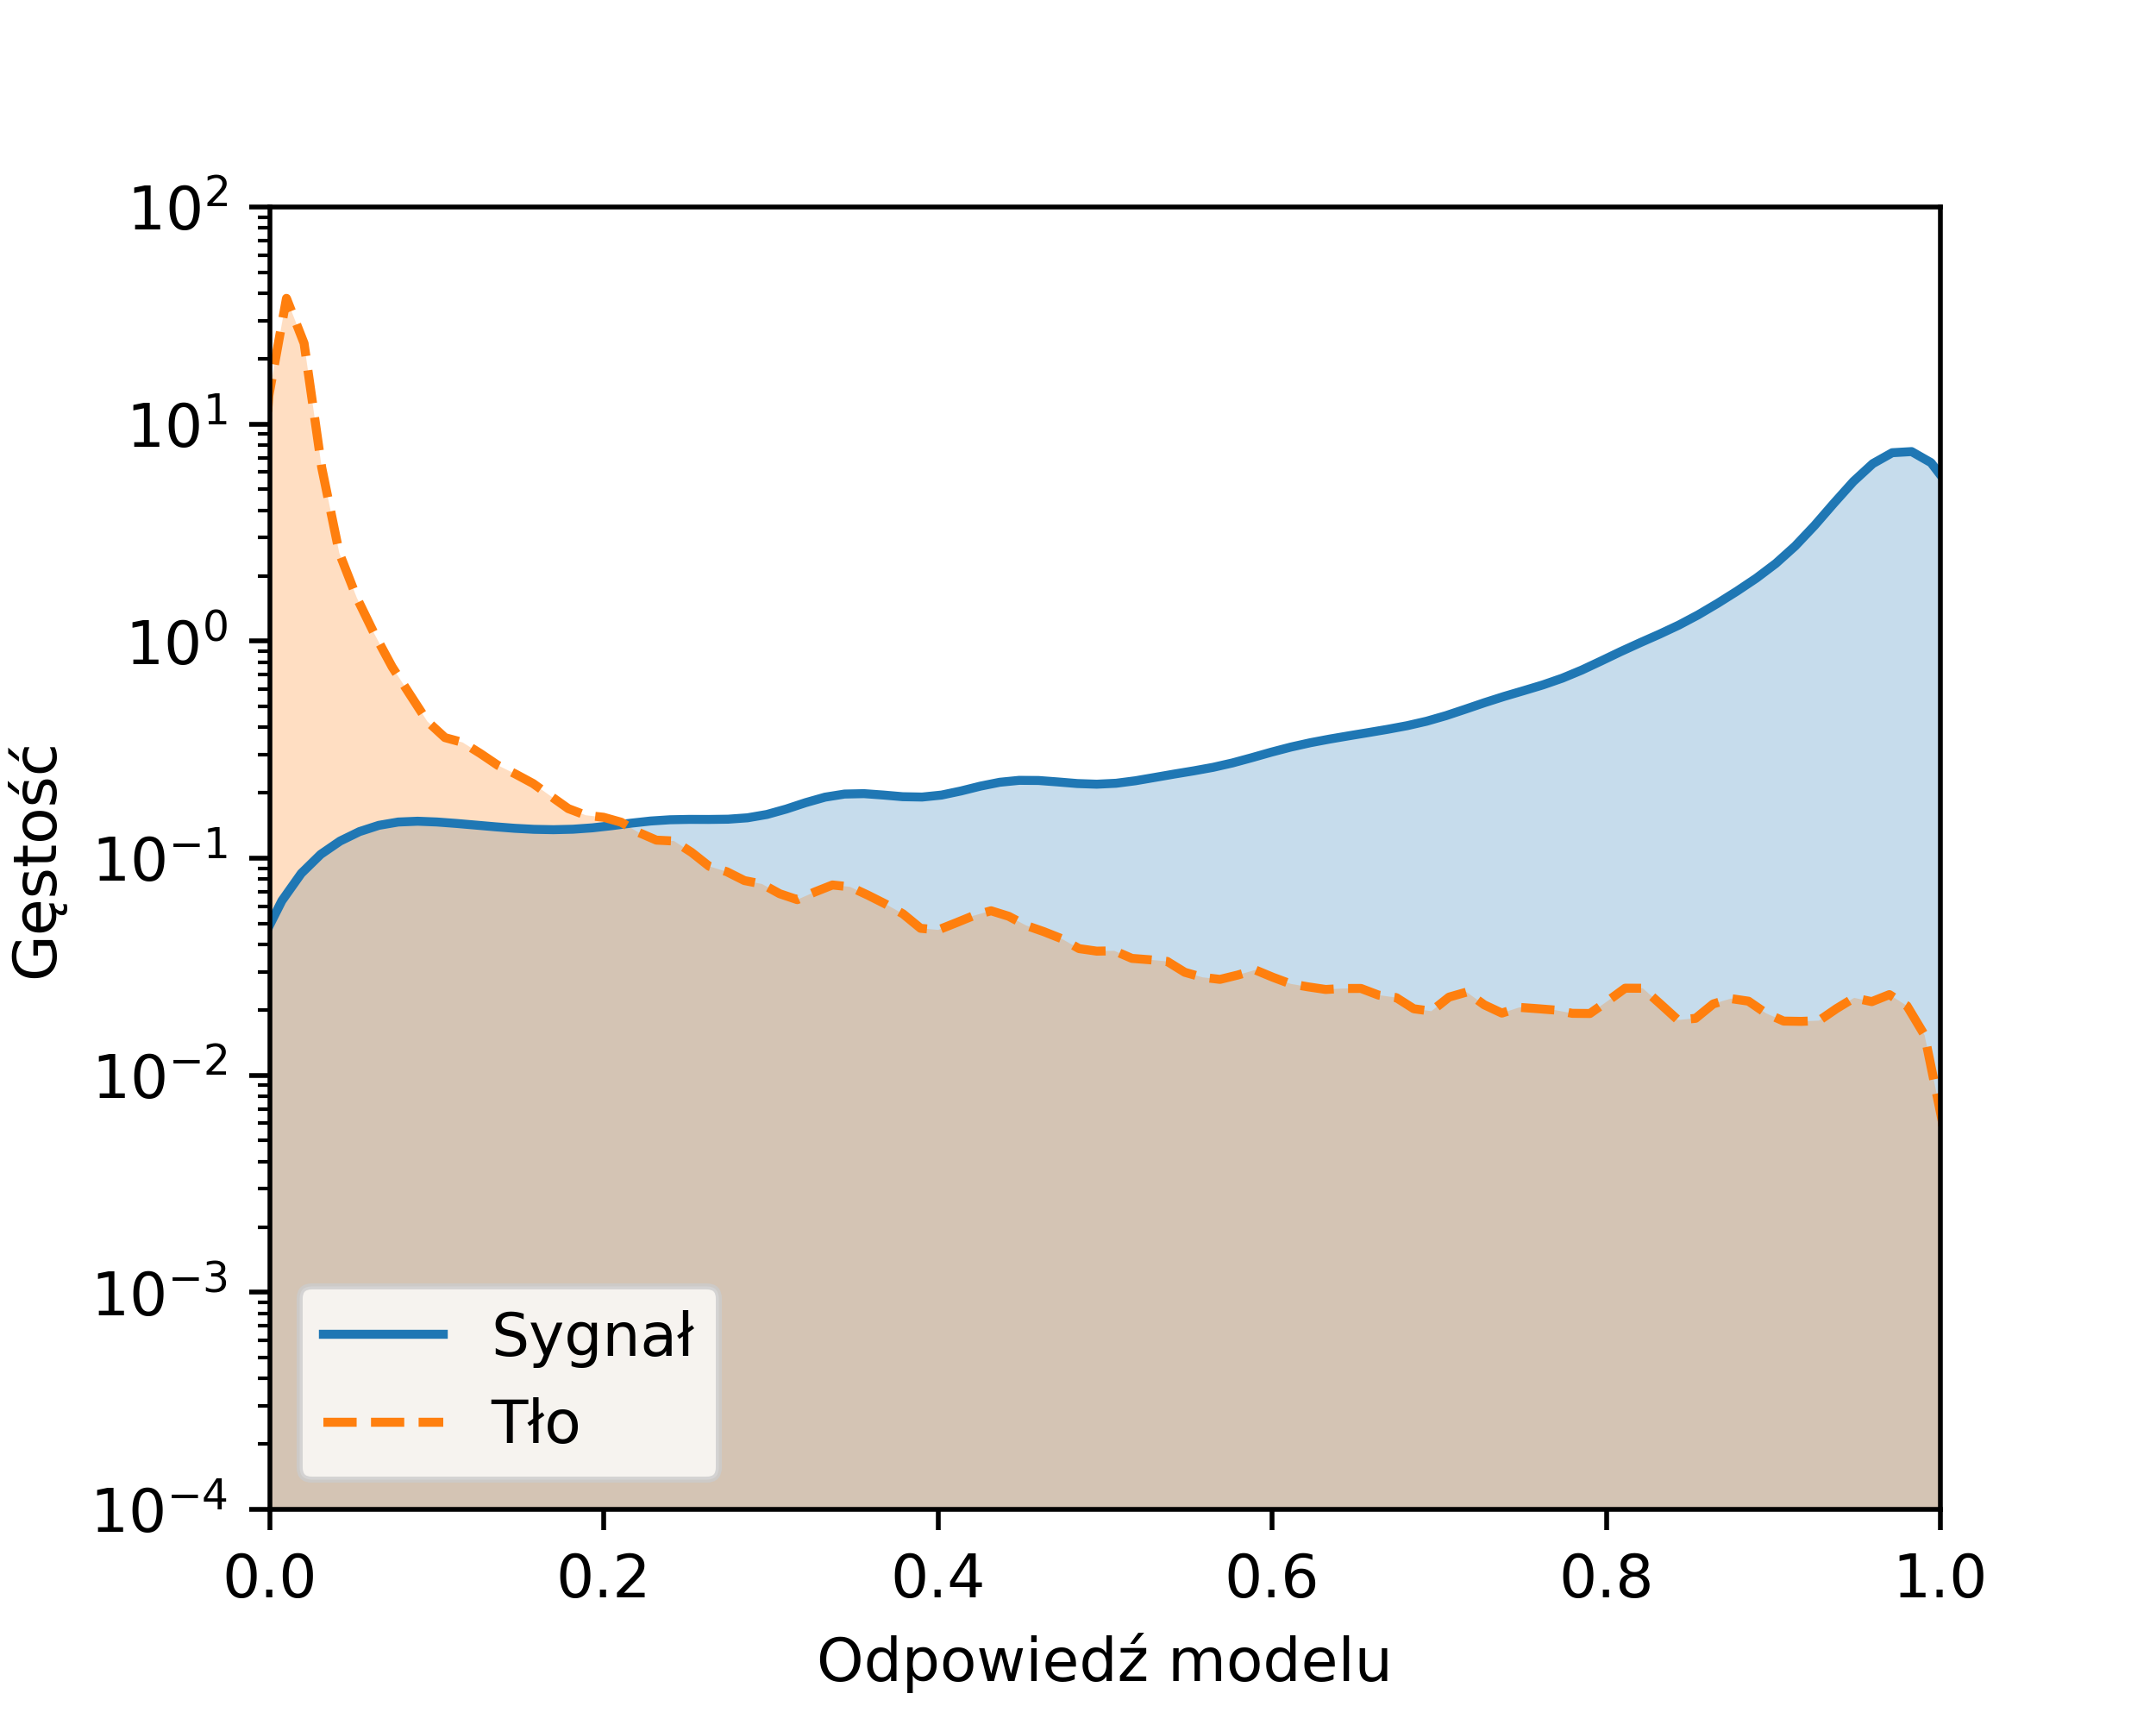
\includegraphics[width=1\textwidth]{density_deepTau.png}
	\caption{\textit{deepTau}}
	\end{subfigure}
	\caption{Rozkłady odpowiedzi modeli dla sygnału i tła. Modele \textit{ensemble}, \textit{baseline} oraz \textit{XGBoost} uczone były na pełnych danych.}
	\label{fig:dist}
	\end{figure}
	\newpage
	Krzywe uczenia dla poszczególnych modeli znajdują się na rysunku \ref{fig:loss}. Dla modeli opartych o sieci neuronowe wykresy przestawiają spadek funkcji straty w zależności od liczby obserwacji na jakiej były uczone. Dodatkowo pionowymi liniami zaznaczono końce kolejnych epok. Natomiast dla \textit{XGBoosta} wykres pokazuje spadek funkcji straty wraz ze wzrostem liczby drzew.
	
	Dla wszystkich modeli widać różnice między wynikiem na zbiorze treningowym, na którym model jest uczony oraz testowym, który służy jedynie do pomiaru skuteczności modeli. Są one niewielkie, co oznacza, że model dobrze generalizuje na nieznane przykłady. Różnice między tymi modelami najlepiej widać na rysunku \ref{fig:loss_all}, gdzie przedstawiono wartość funkcji straty na zbiorze testowym dla modeli opartych na sieciach. Model \textit{XGBoost} nie jest na nim przedstawiony, ponieważ jego krzywa uczenia nie może być bezpośrednio porównywana z krzywymi uczenia sieci neuronowych. 
	
	Można zauważyć, że funkcja straty dla modelu \textit{ensemble} maleje wolniej niż dla modeli \textit{baseline} oraz \textit{best-nn}. Natomiast dla modelu \textit{baseline} ma ona większą wariancję niż dla pozostałych. Krzywe mocno się wypłaszczają wraz z treningiem, jednak widać, że dla modeli \textit{baseline} oraz \textit{best-nn} potencjalnie trening można wydłużyć.
	
	\begin{figure}
	\begin{subfigure}{.5\textwidth}
	\centering
	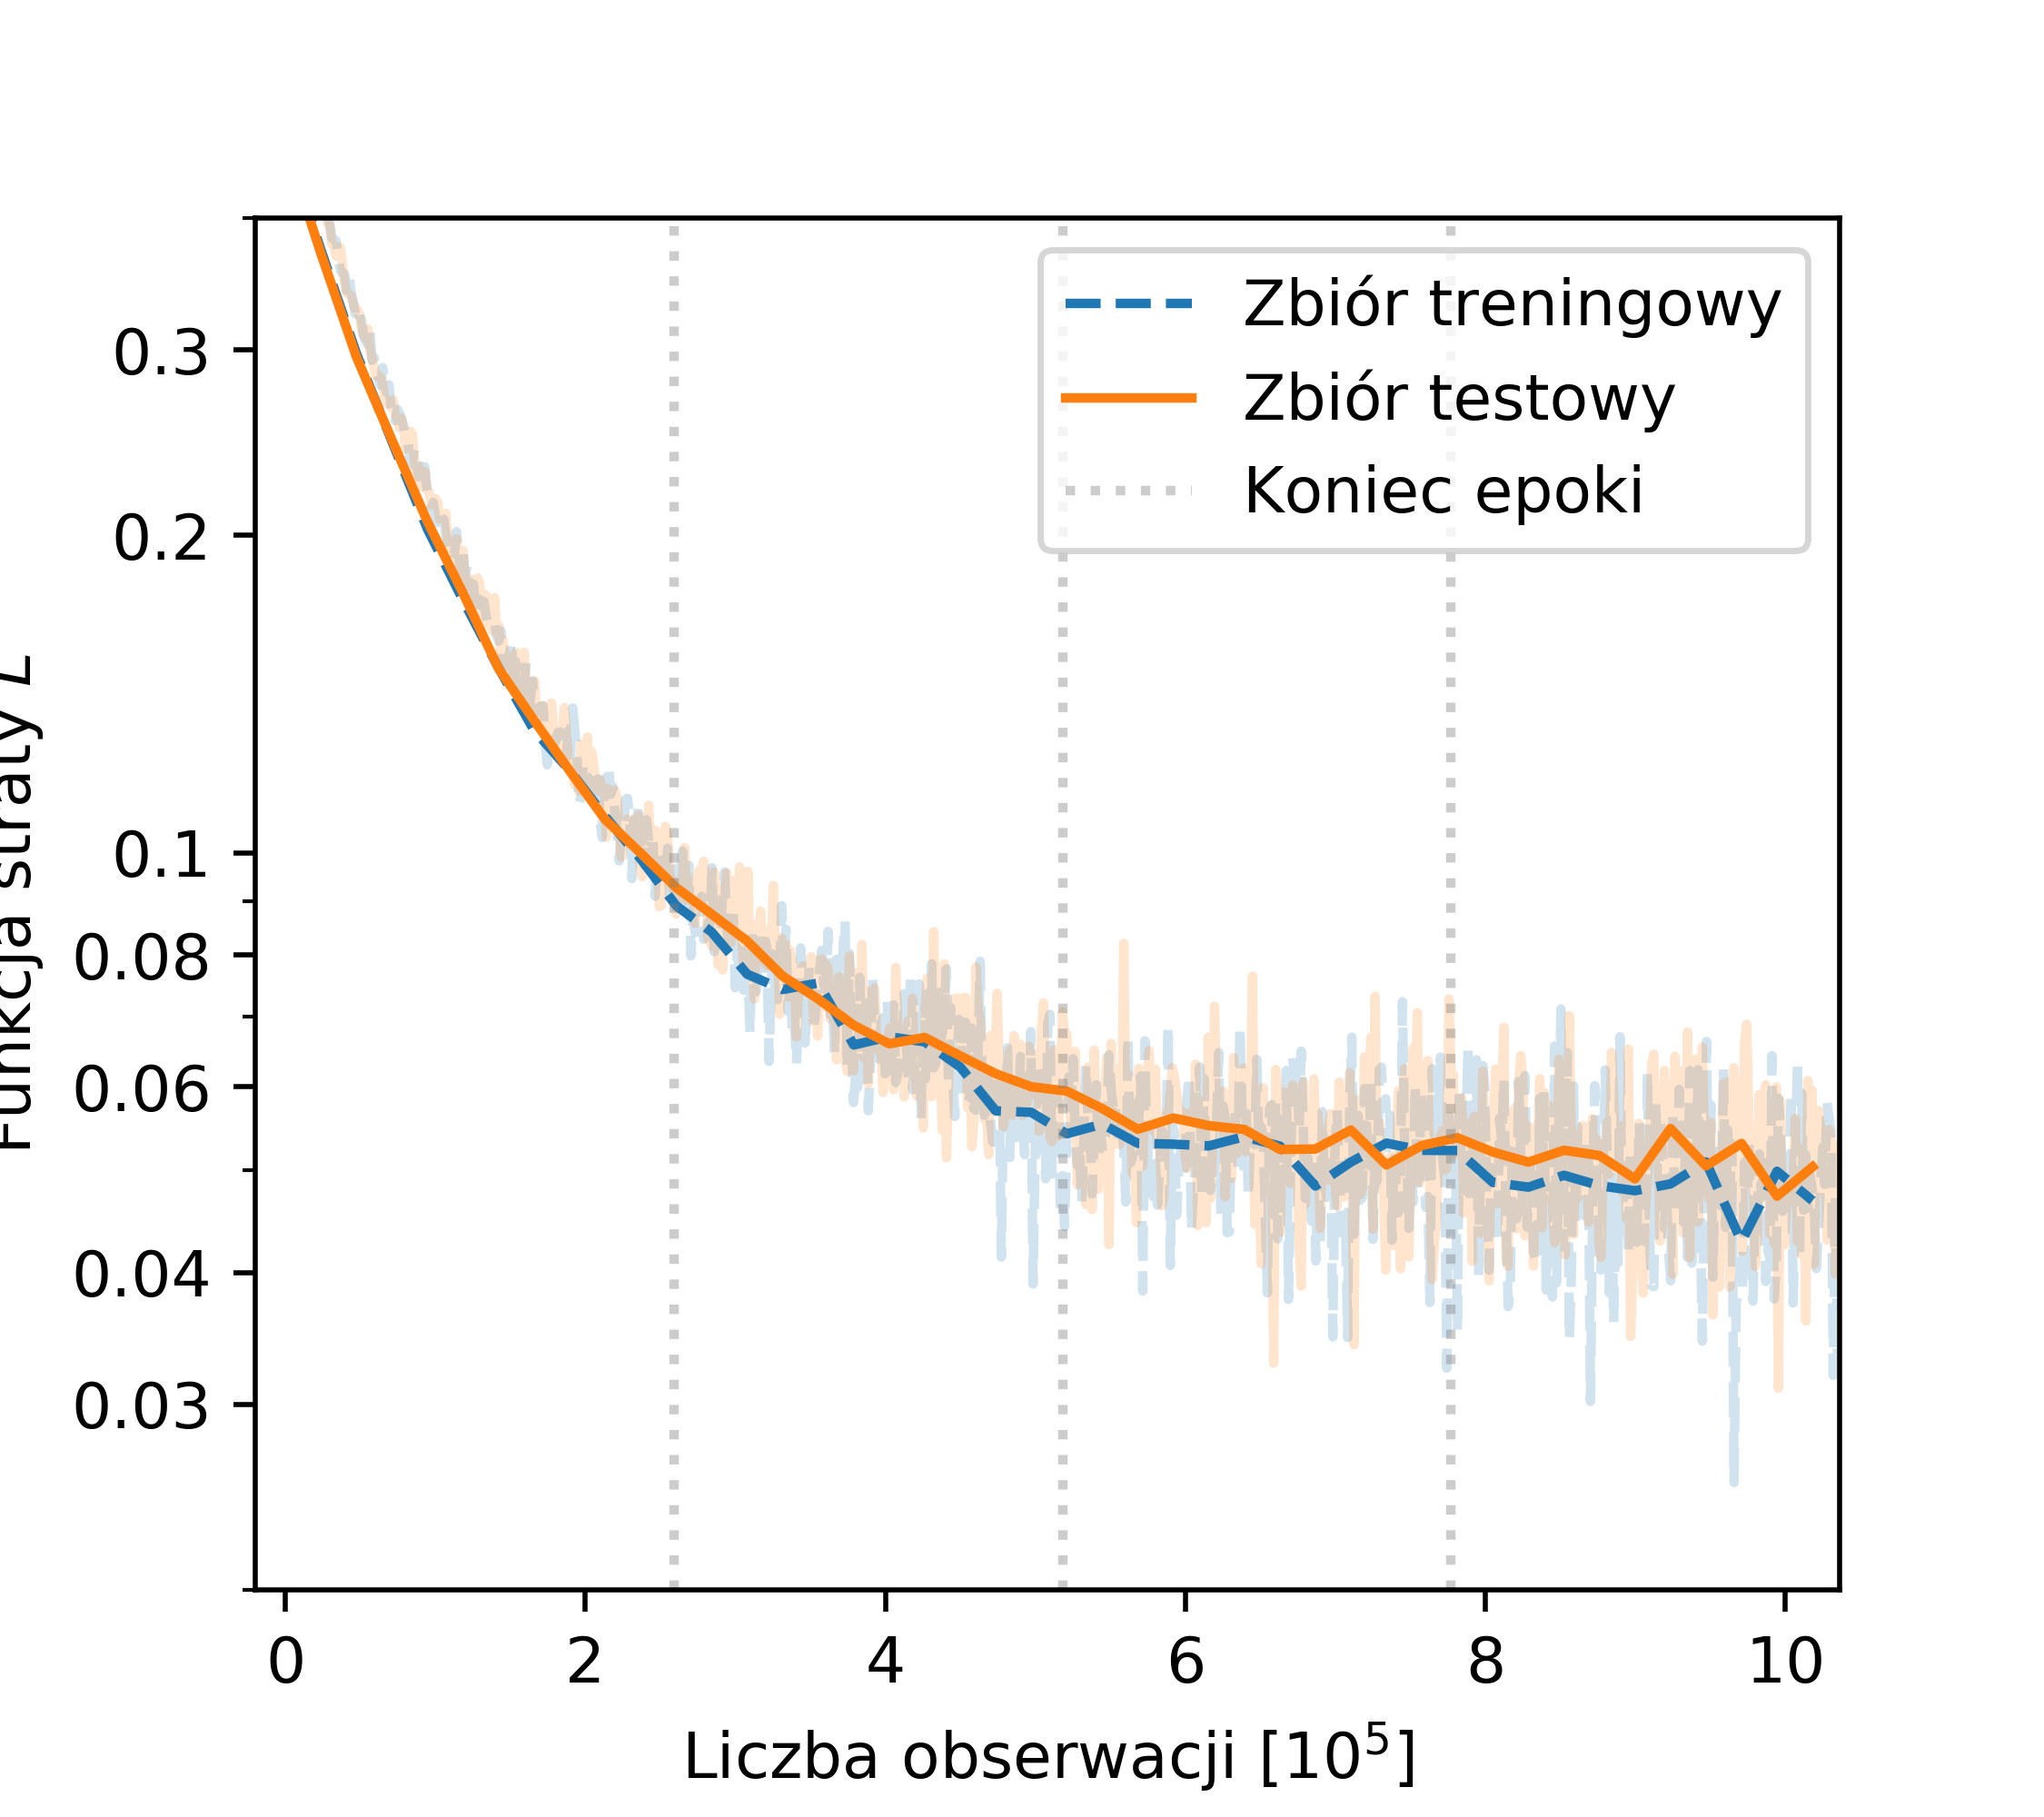
\includegraphics[width=1\textwidth]{loss_ensemble.png}
	\caption{\textit{ensemble}}
	\end{subfigure}
	\begin{subfigure}{.5\textwidth}
	\centering
	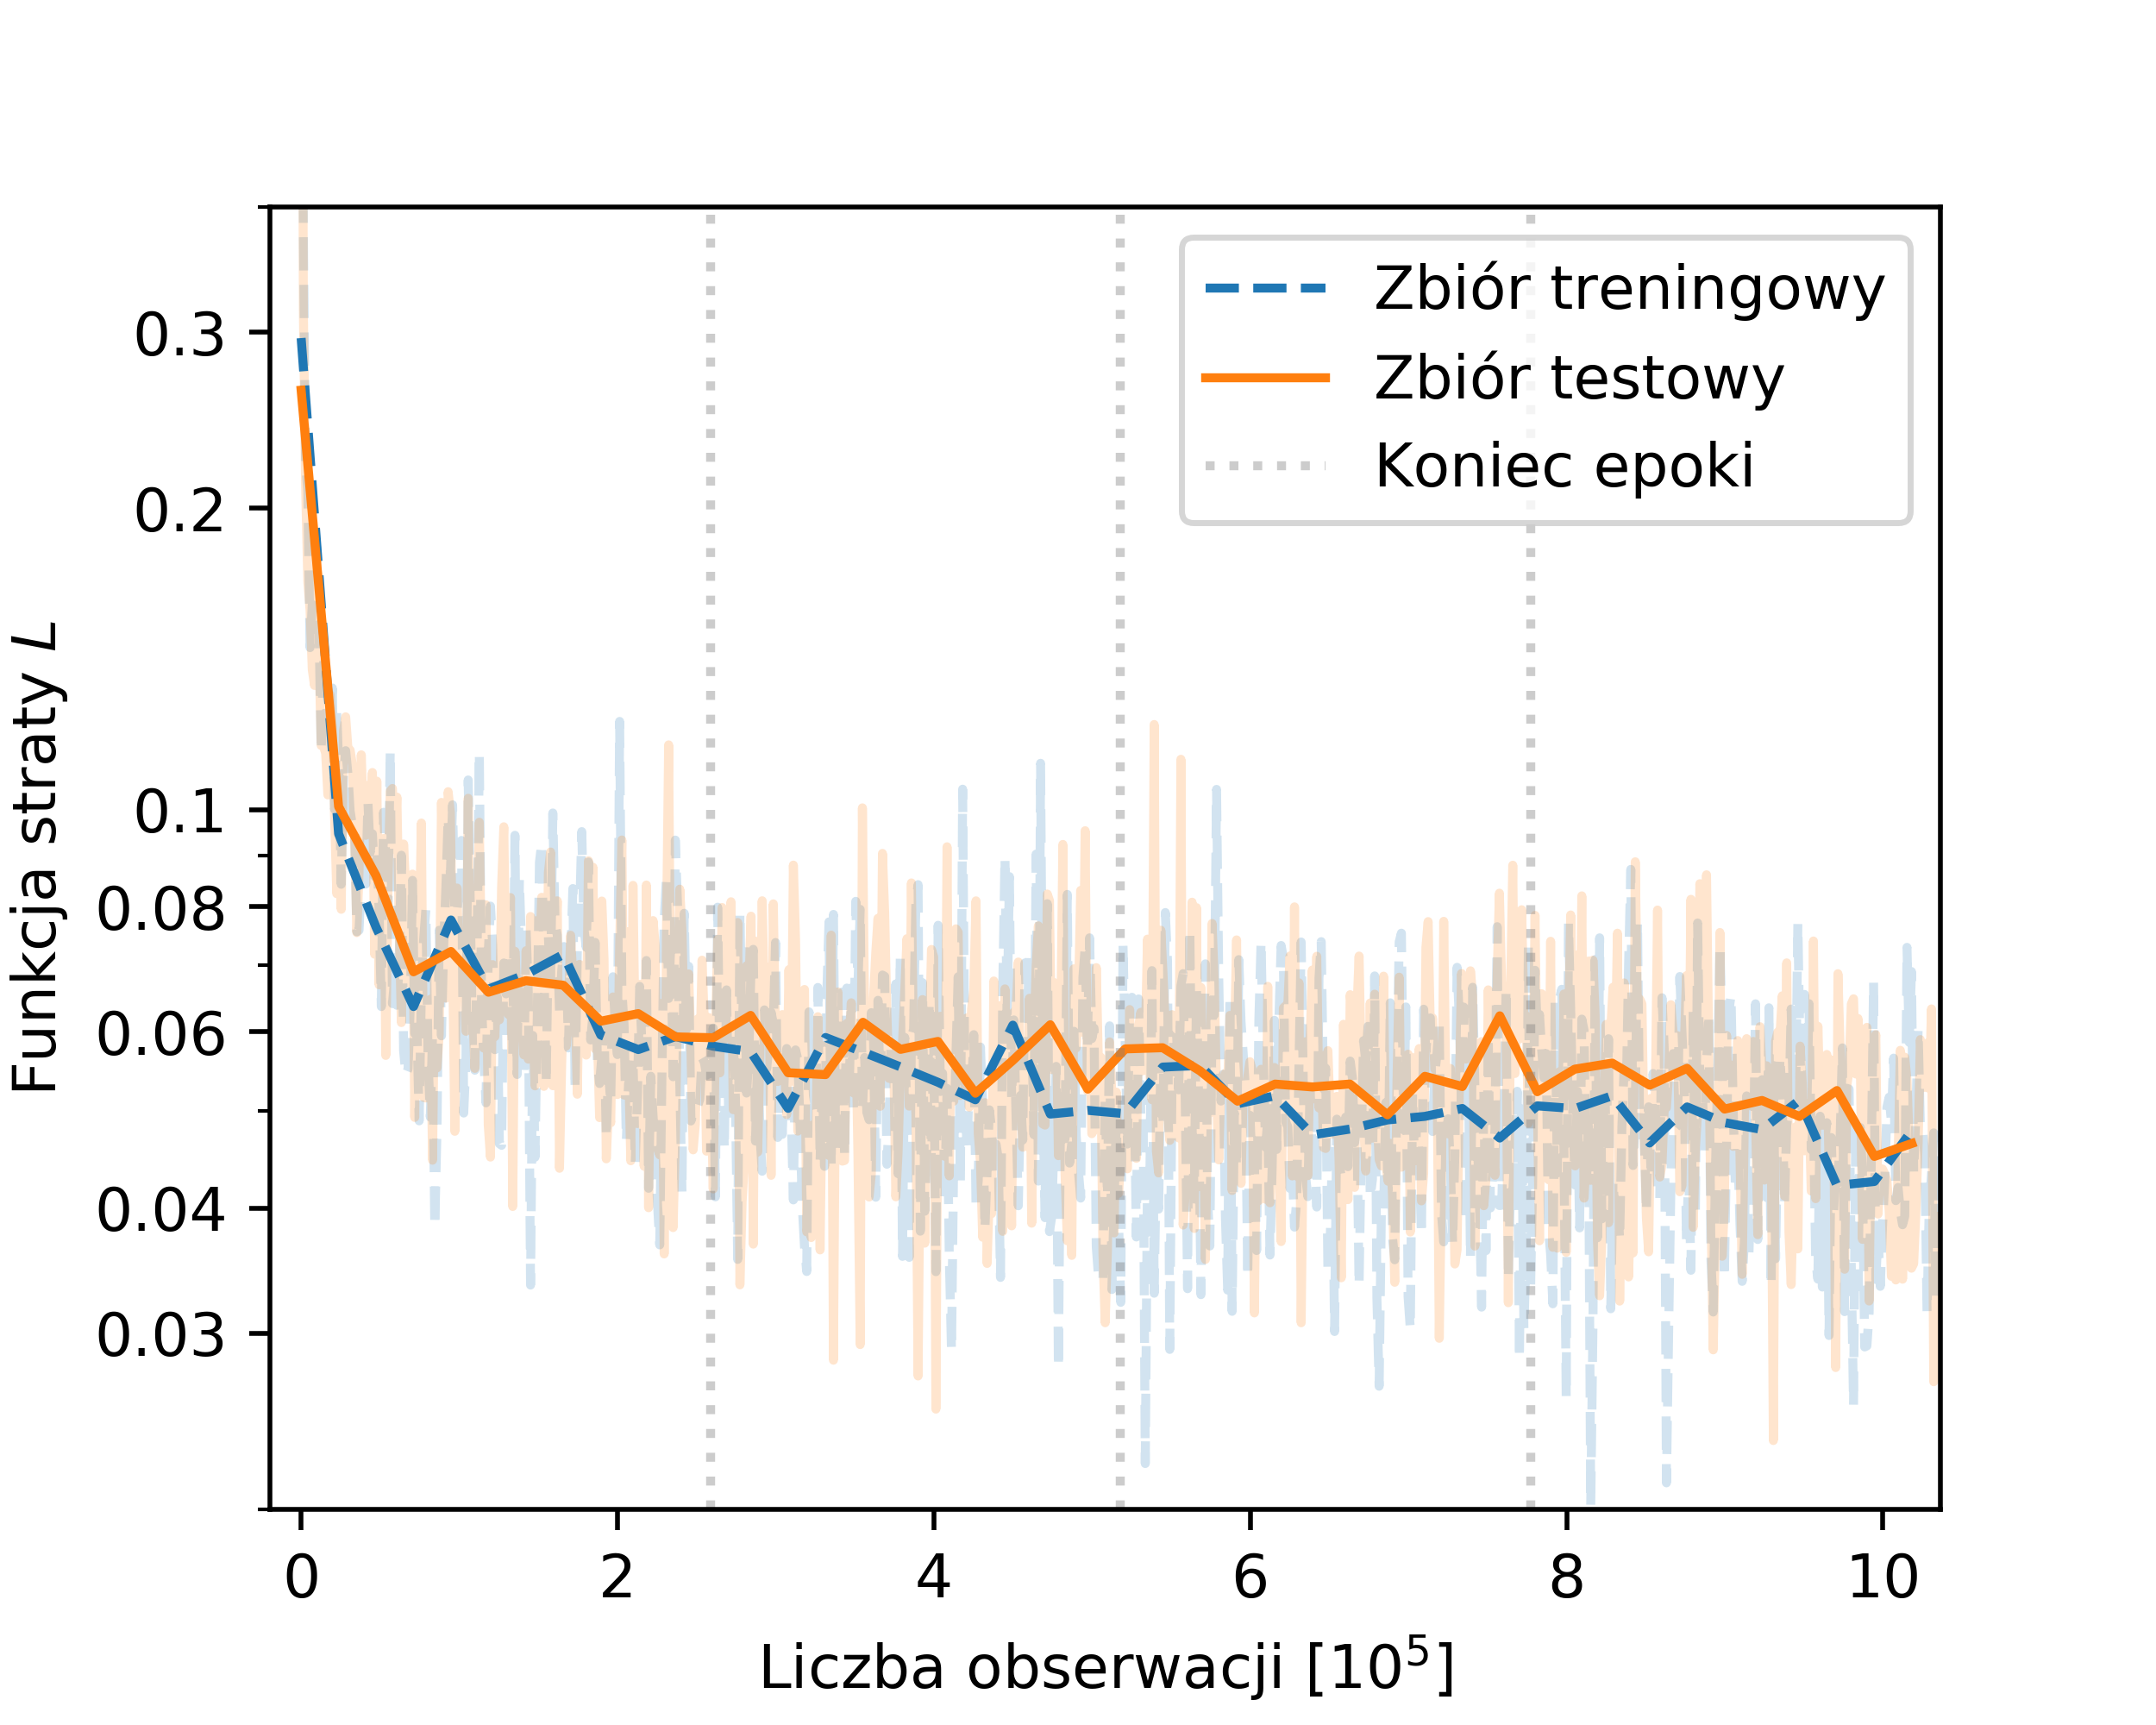
\includegraphics[width=1\textwidth]{loss_baseline.png}
	\caption{\textit{baseline}}
	\end{subfigure}
	\begin{subfigure}{.5\textwidth}
	\centering
	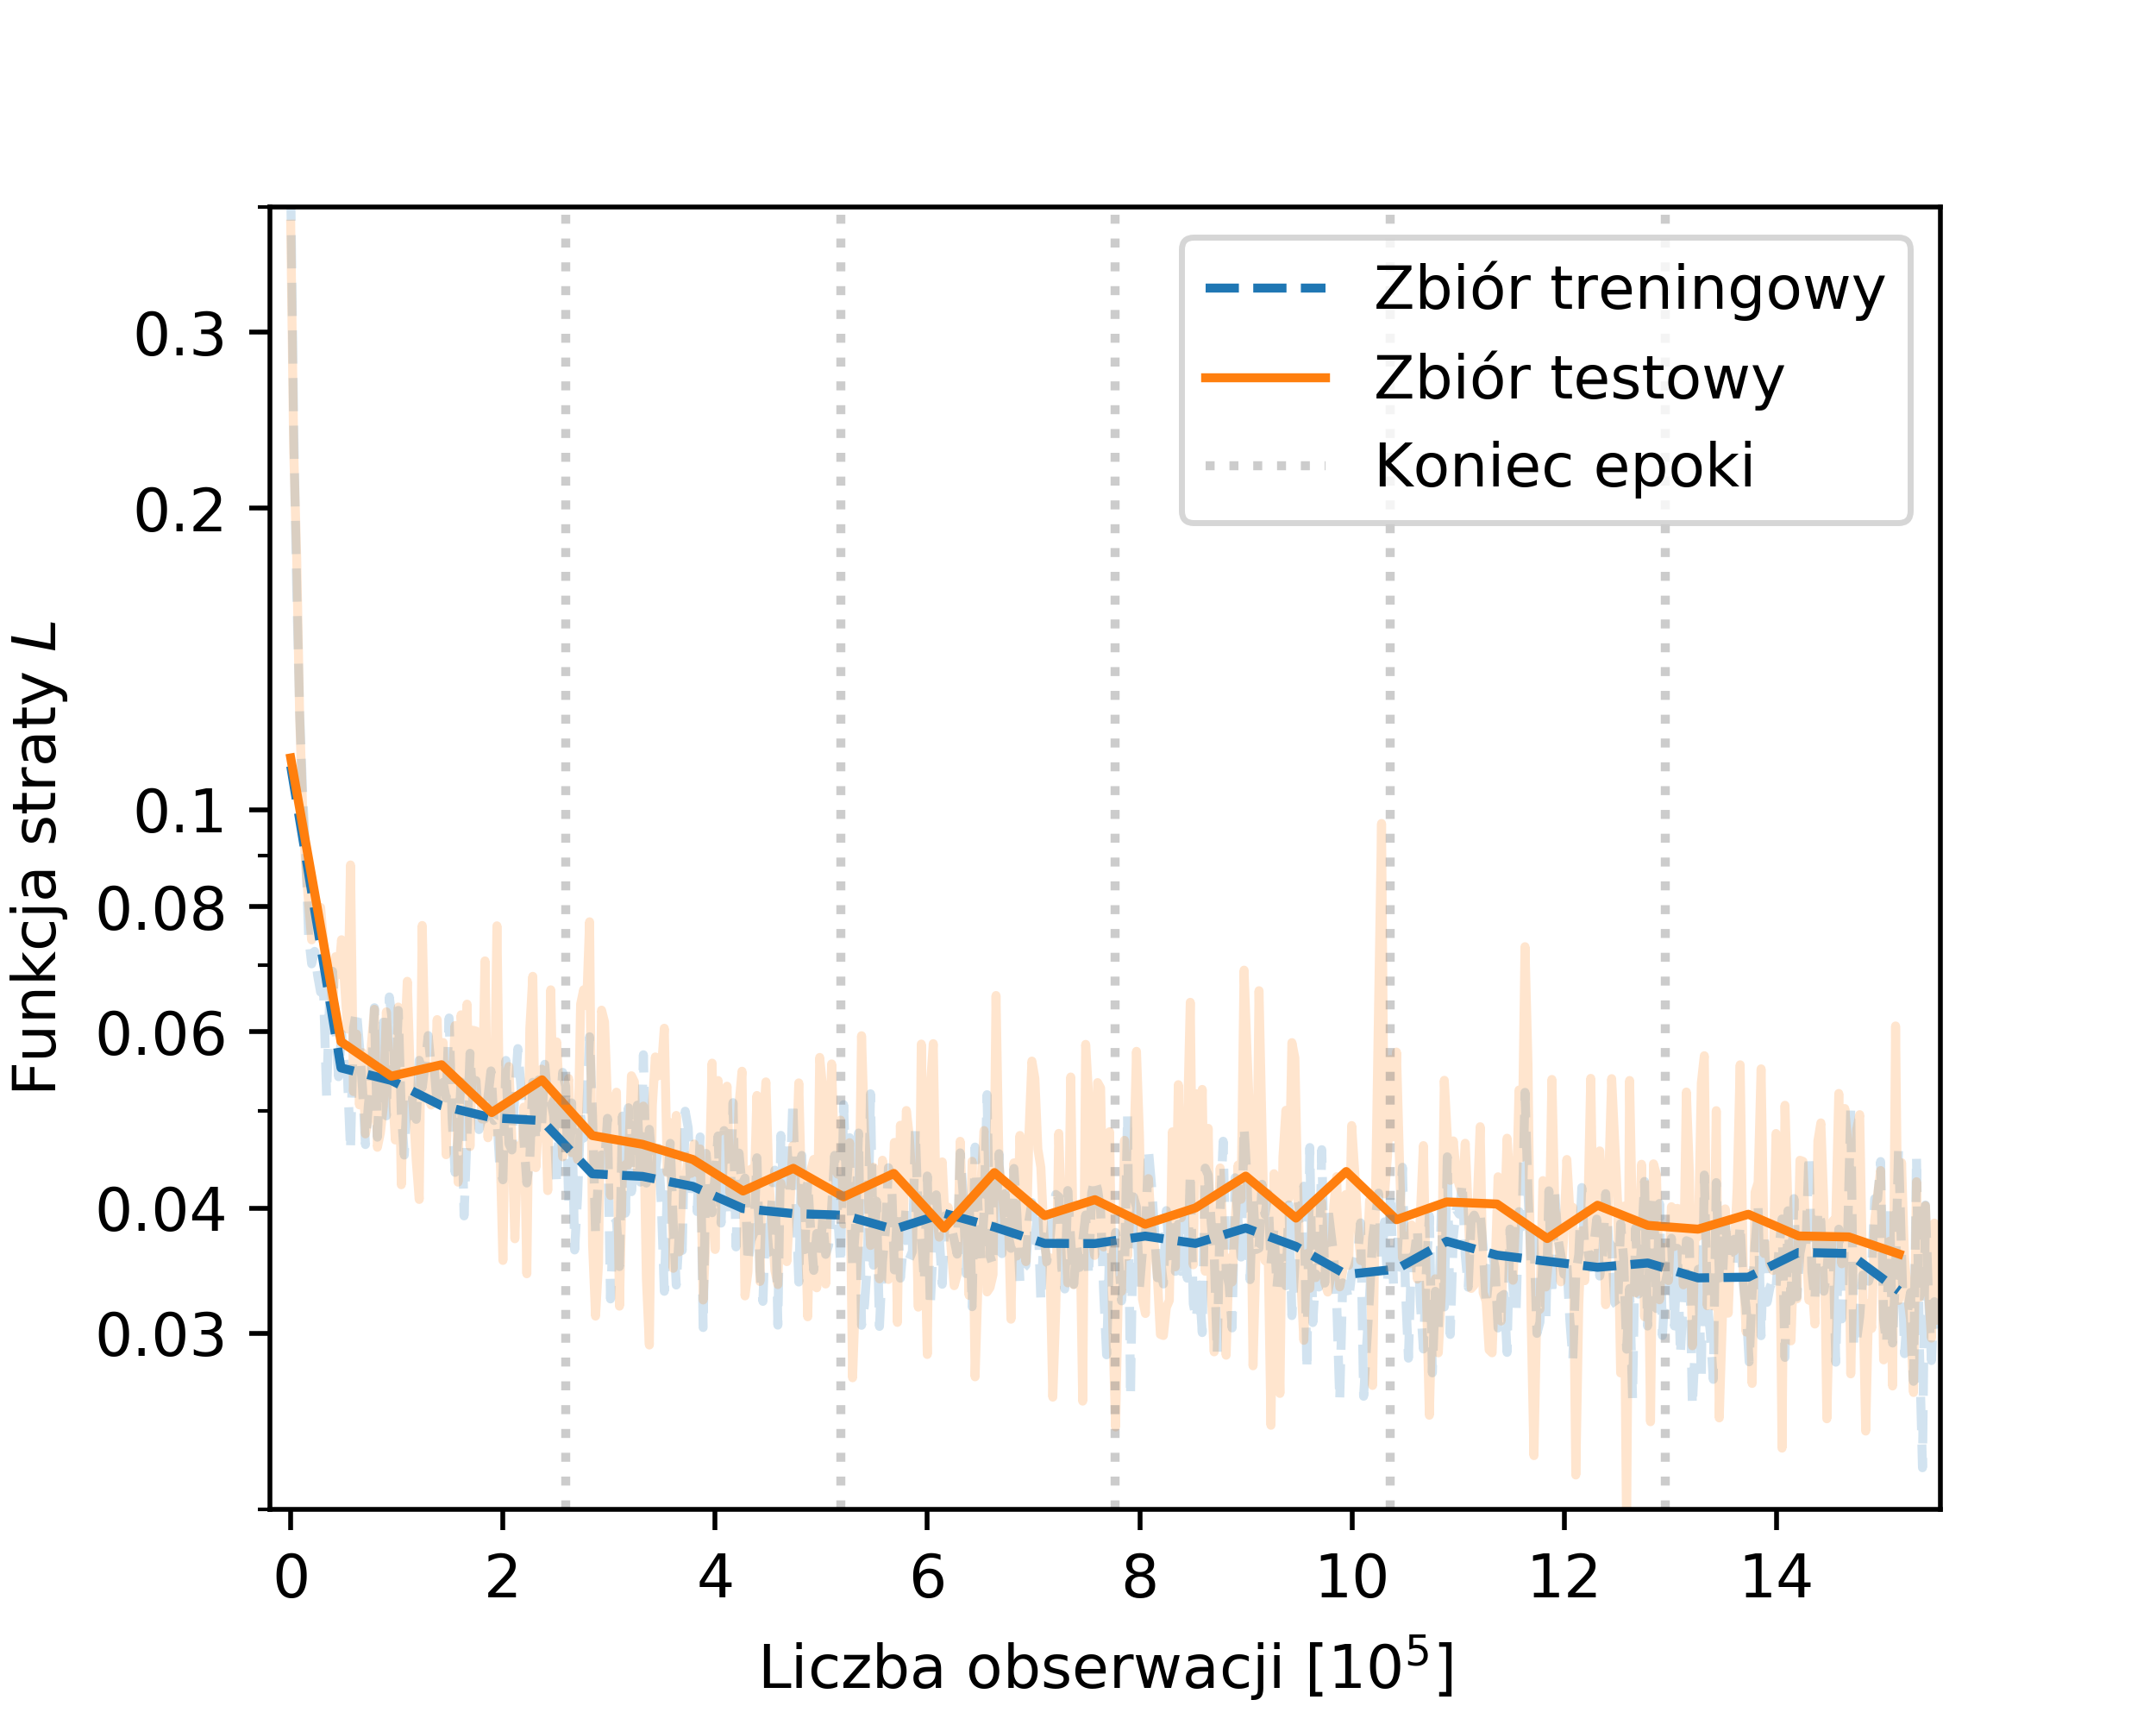
\includegraphics[width=1\textwidth]{loss_best-nn.png}
	\caption{\textit{best-nn}}
	\end{subfigure}
	\begin{subfigure}{.5\textwidth}
	\centering
	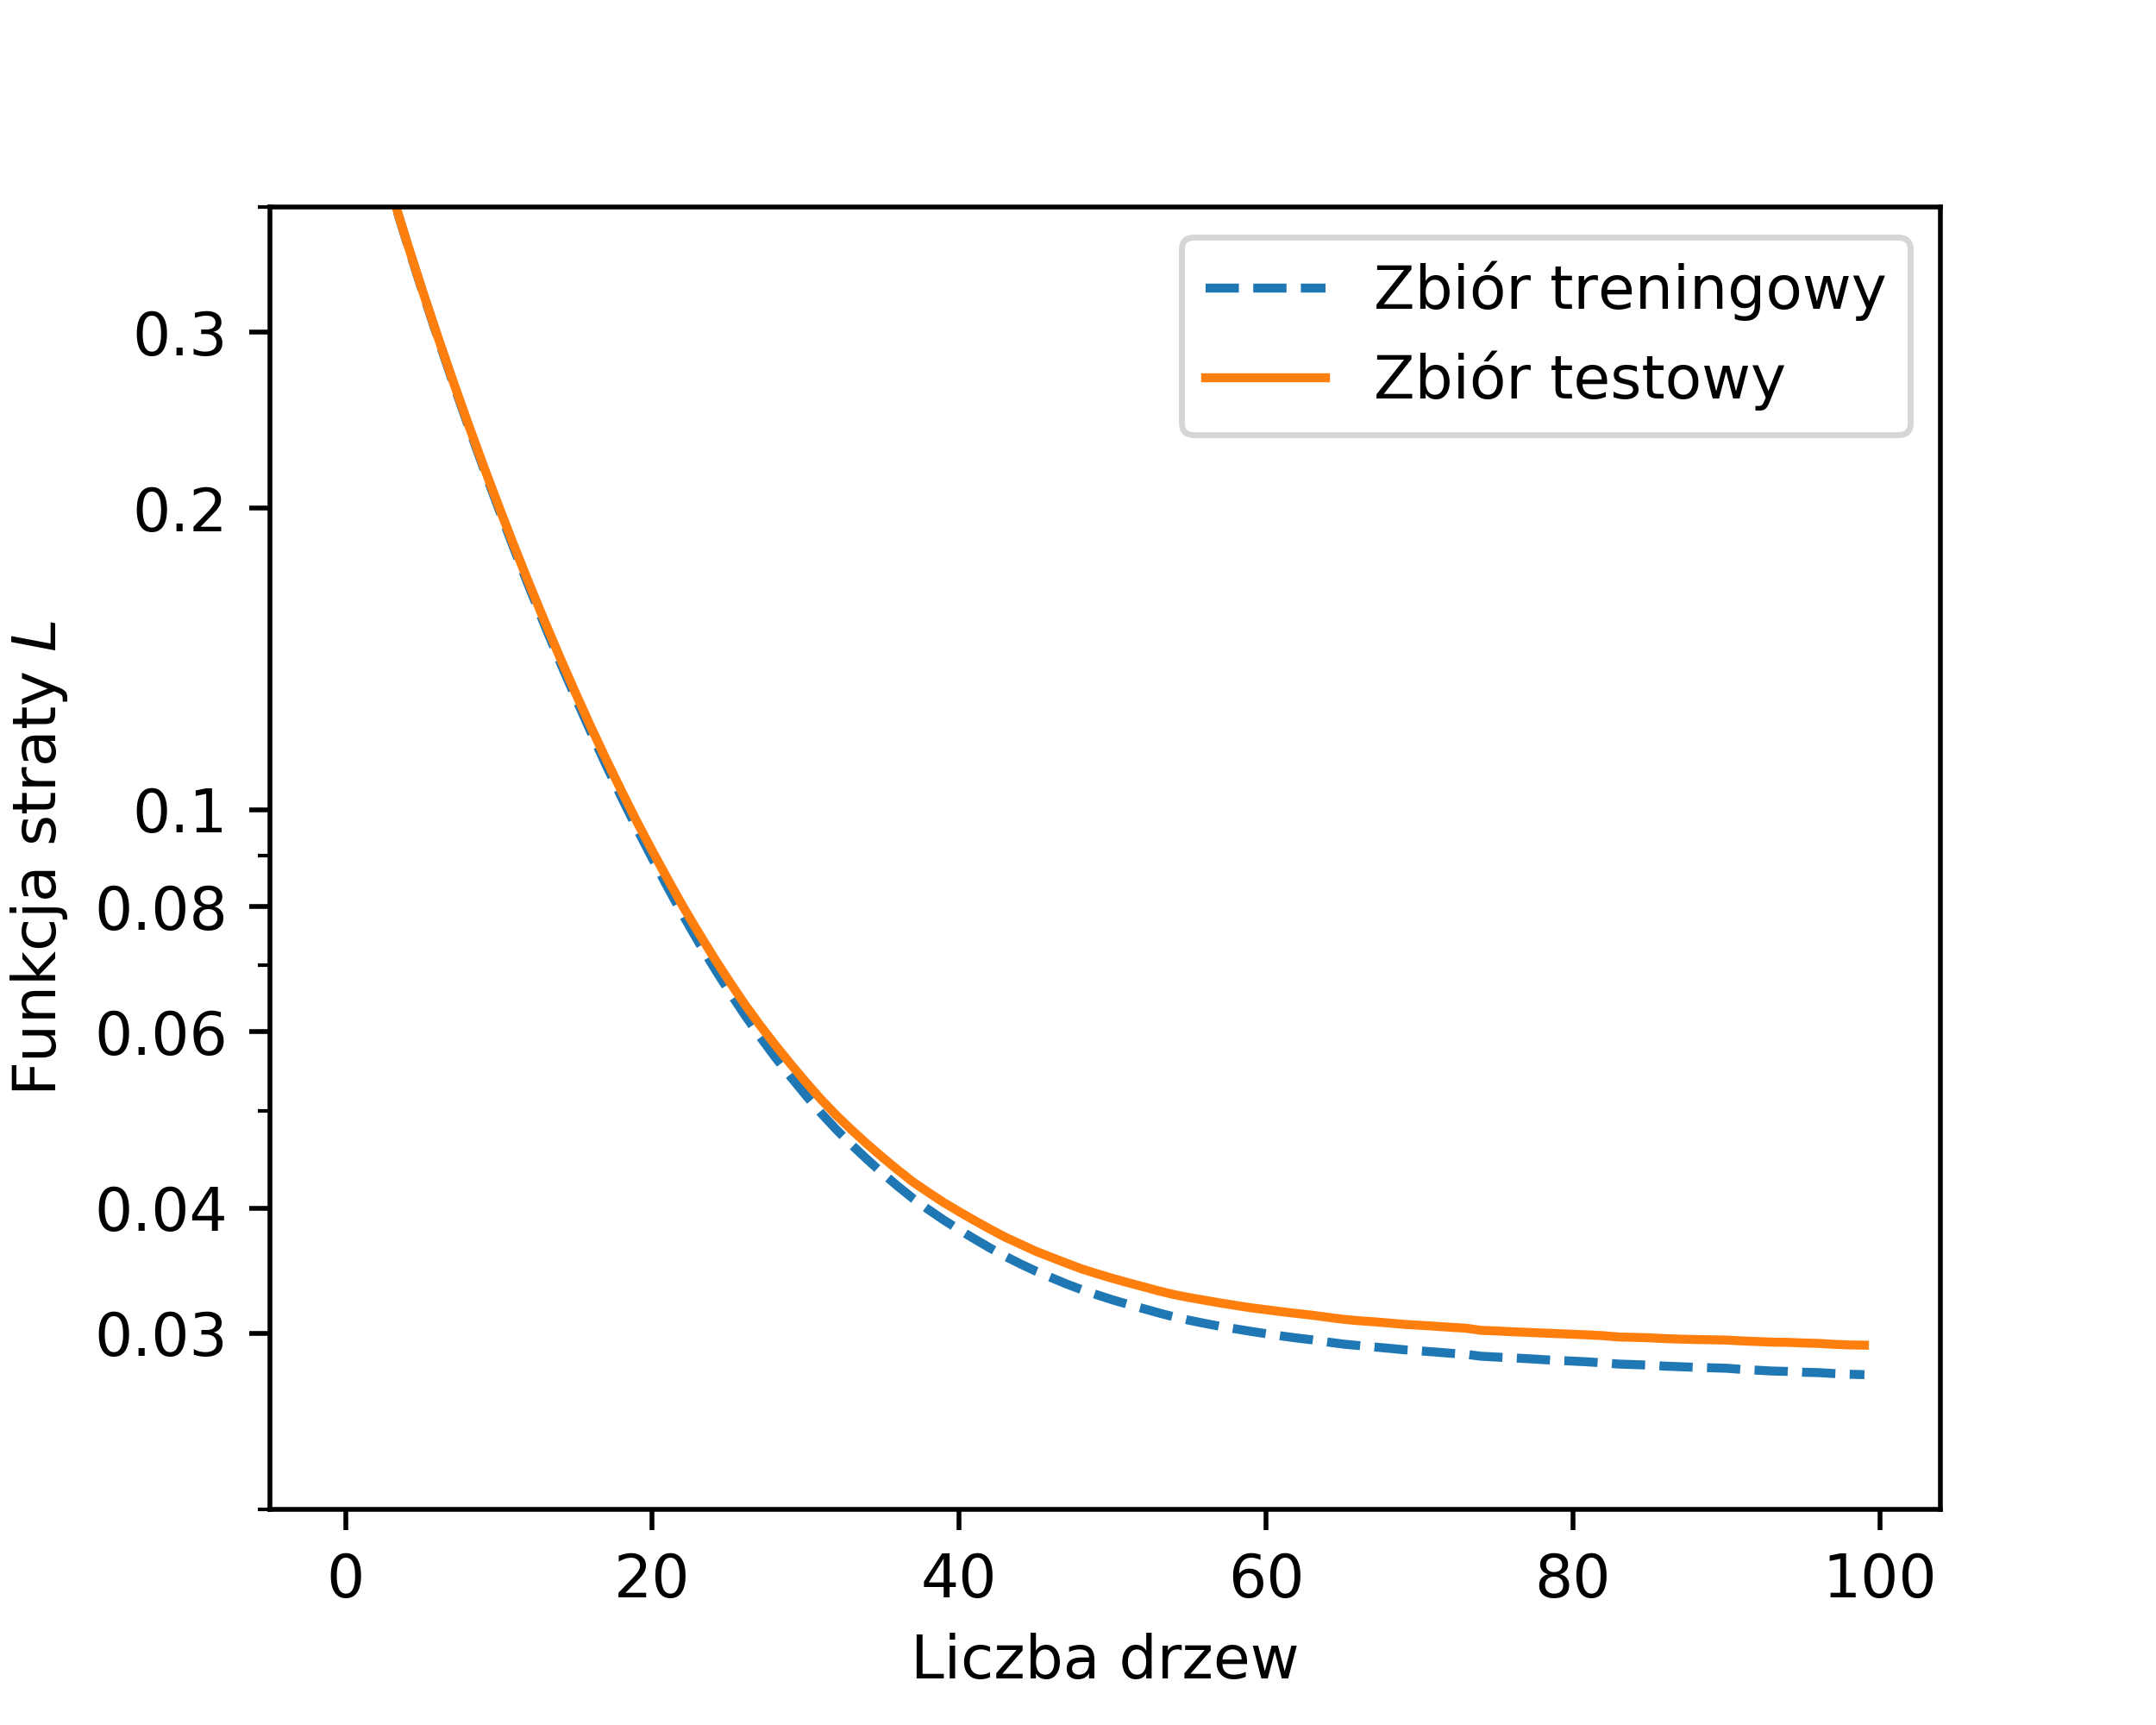
\includegraphics[width=1\textwidth]{loss_xgb.png}
	\caption{\textit{XGBoost}}
	\end{subfigure}
	\caption{Zmiana wartości funkcji straty liczona na zbiorze testowym dla wszystkich modeli. Dla modeli opartych o sieci neuronowe, na osi x znajduje się liczba obserwacji, a dla \textit{XGBoosta} liczba dopasowanych drzew. Modele \textit{ensemble}, \textit{baseline} oraz \textit{XGBoost} uczone były na pełnych danych.}
	\label{fig:loss}
	\end{figure}	
	
	\begin{figure}
	\centering
	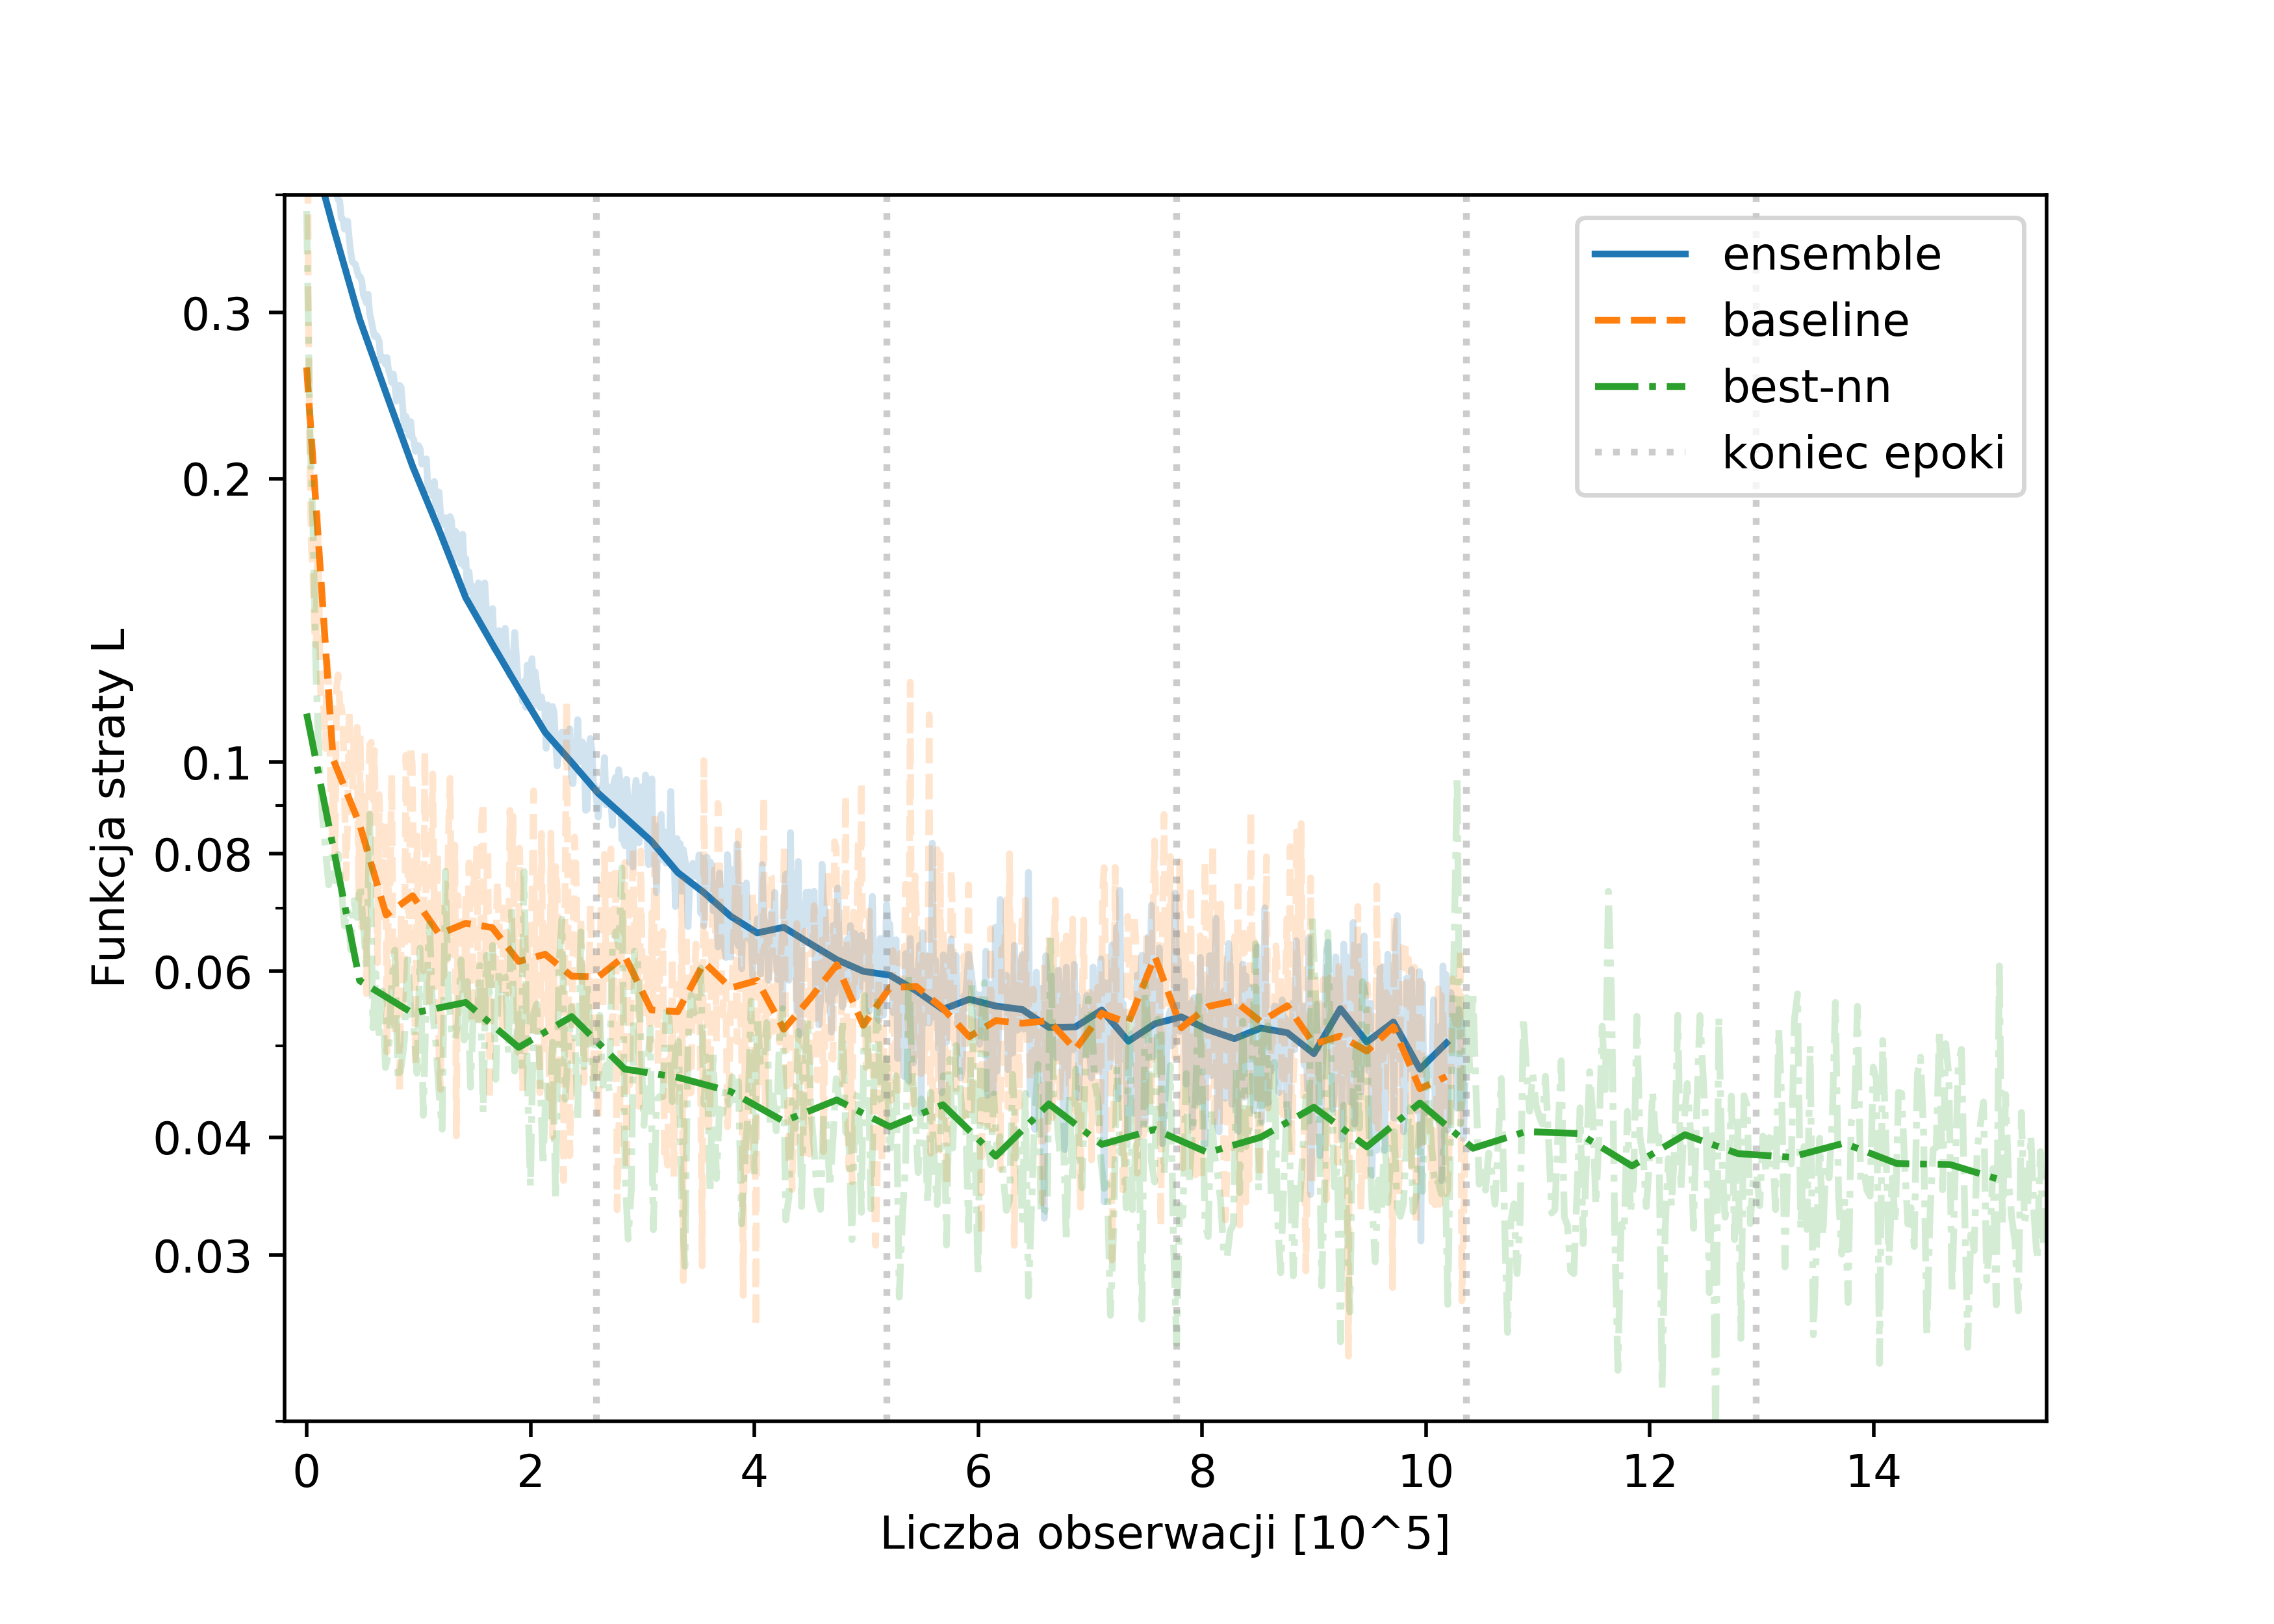
\includegraphics[width=1.\textwidth]{loss_all.png}
	\caption{Zmiana wartości funkcji straty od liczby obserwacji liczona na zbiorze testowym dla wszystkich modeli opartych o sieci neuronowe.}
	\label{fig:loss_all}
	\end{figure}	
	%\newpage
	Na rysunkach \ref{fig:res_best}, \ref{fig:res_new} i \ref{fig:res_disc} przedstawiono fragmenty krzywych ROC dla wybranych modeli. Zakres TPR na wykresach został zmniejszony, aby lepiej uwidocznić różnice między modelami.
	
	\begin{figure}
	\centering
	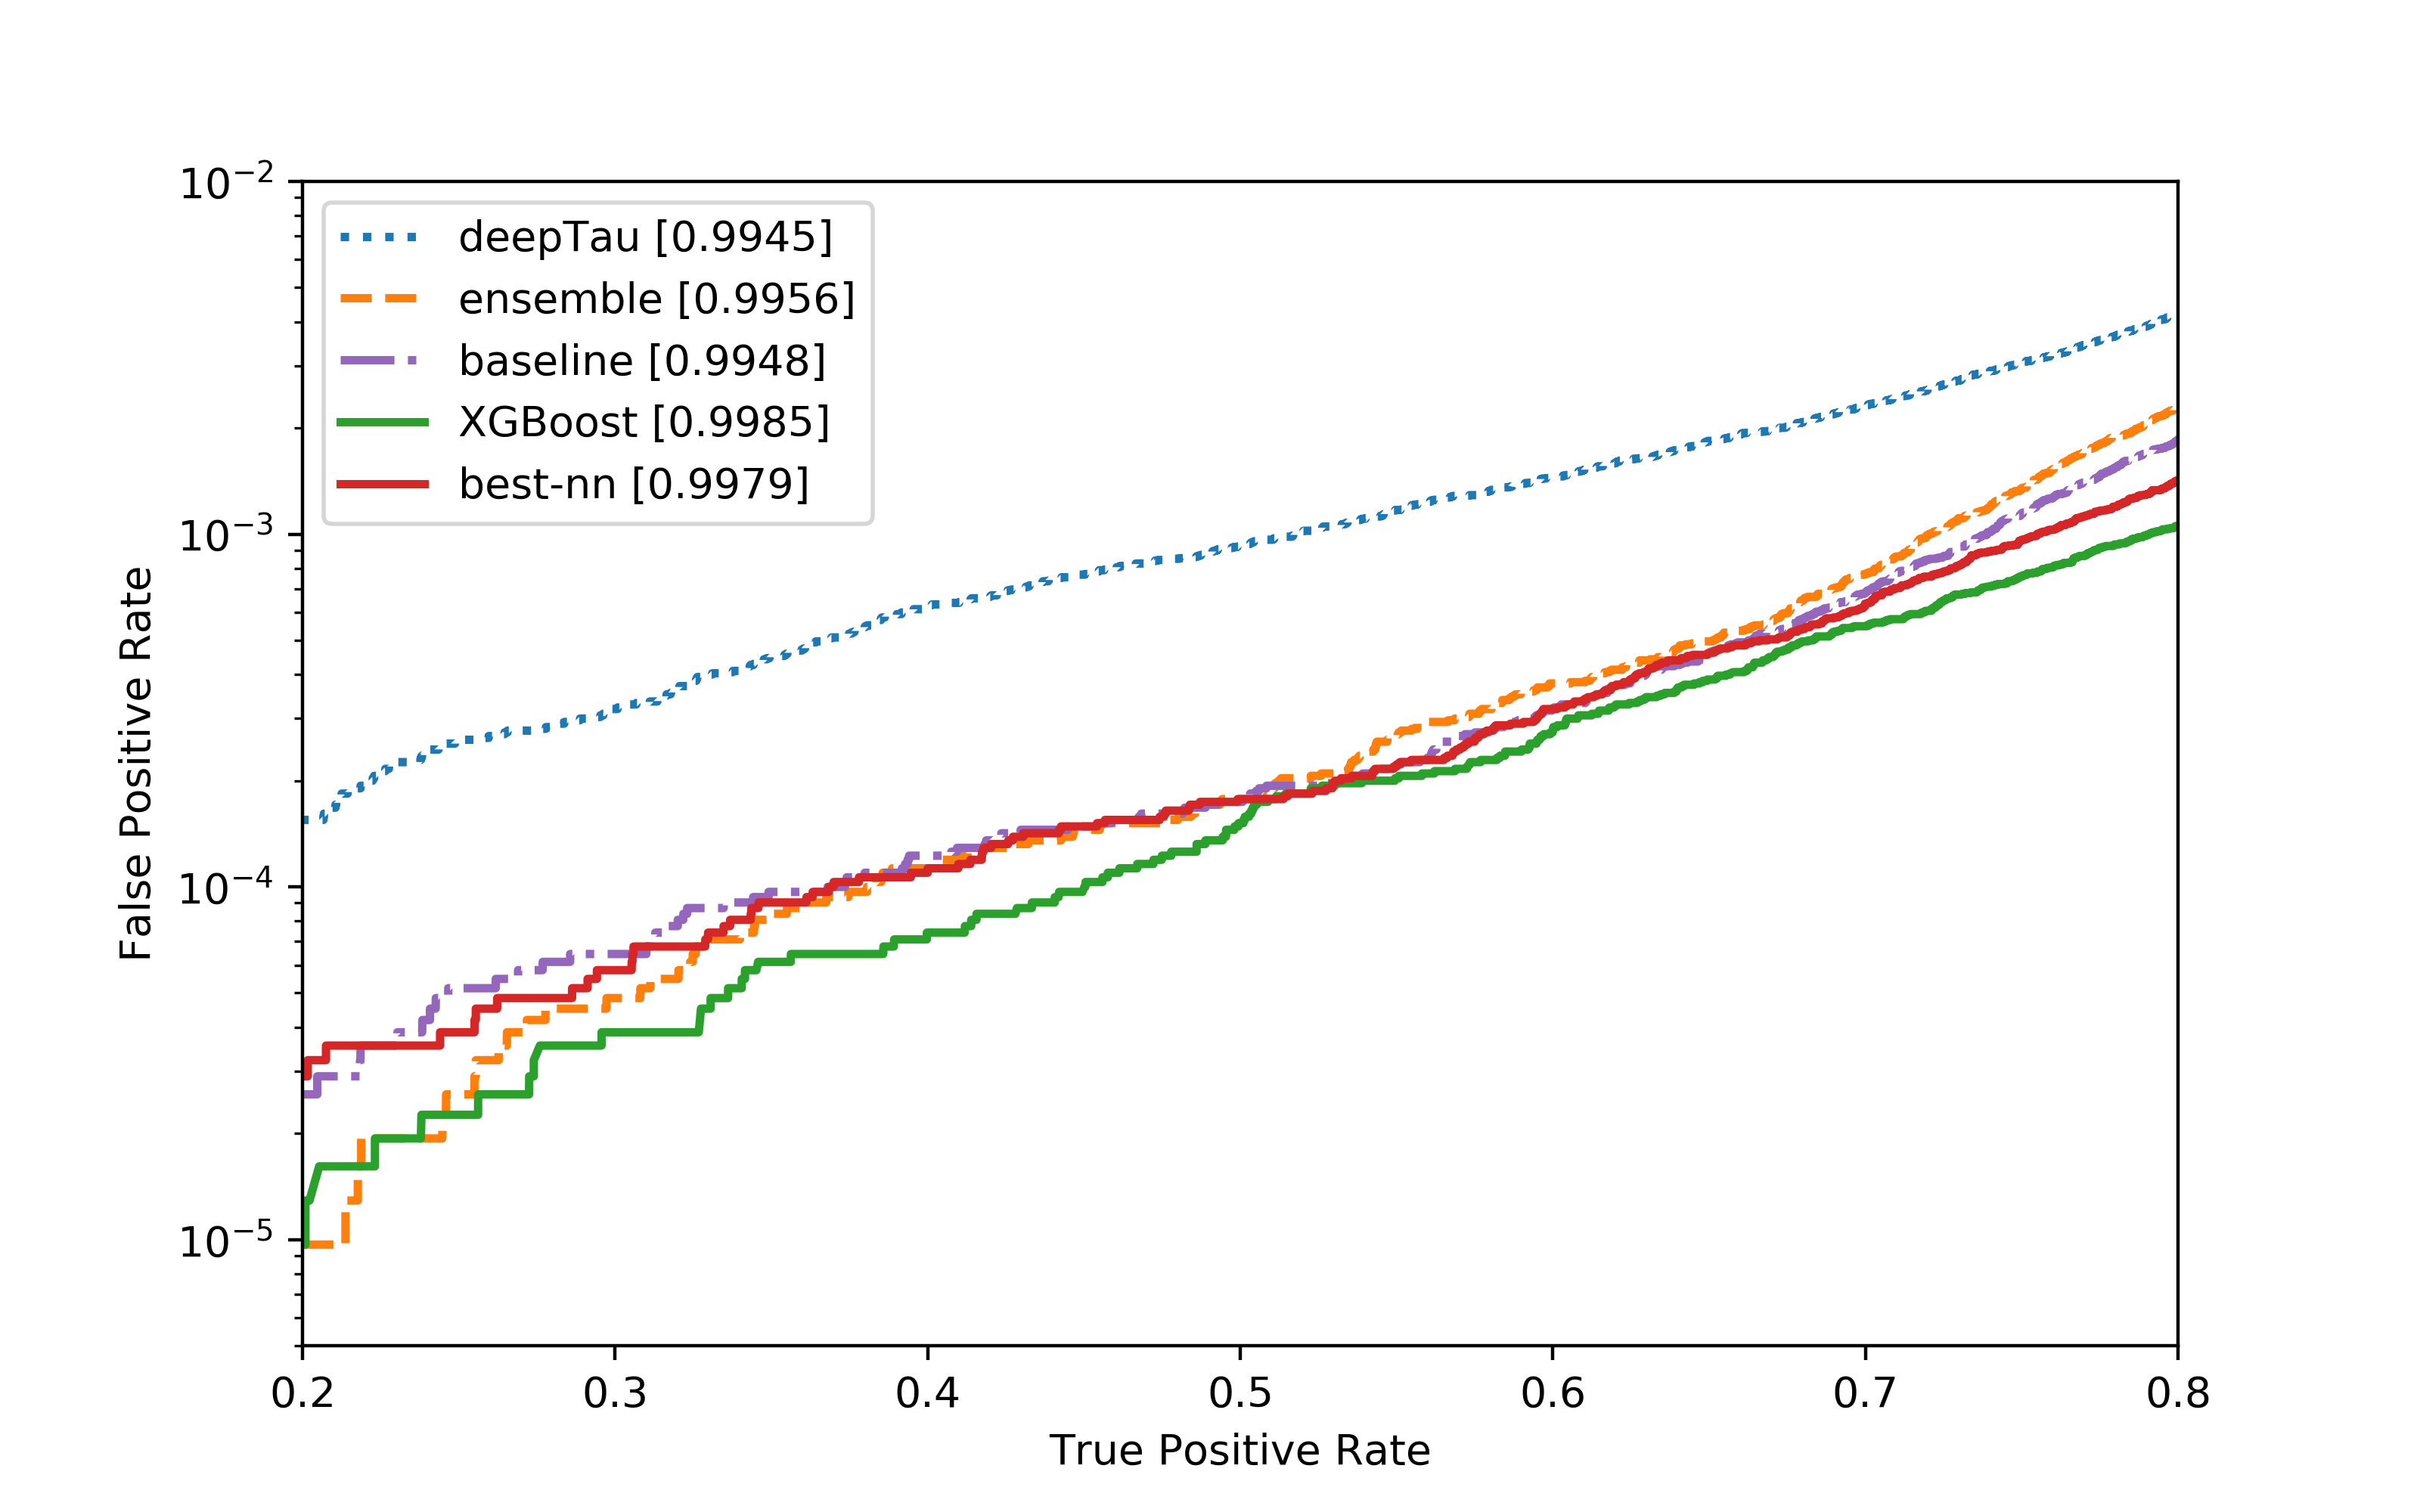
\includegraphics[width=1\textwidth]{best_models.png}
	\caption{Porównanie najlepszych modeli na podstawie krzywej ROC.  \textit{baseline}, \textit{best-nn} oraz \textit{XGBoost} były uczone na pełnych danych, a \textit{deepTau} na danych bez klasyfikatorów. W nawiasach kwadratowych podano wartość ROC AUC dla danego modelu.}
	\label{fig:res_best}	
	\end{figure}
	
	Rysunek \ref{fig:res_best} przedstawia krzywe ROC dla najlepszego modelu każdego typu. Można zauważyć, że największa różnica jest między \textit{deepTau} a innymi modelami, natomiast najskuteczniejszy jest \textit{XGBoost}. Pomimo tego, że różnice w ROC AUC są niewielkie dla wszystkich modeli, to jeśli punkt odcięcia zostałby wybrany tak, aby TPR był równy 0.5 (model wykrywa połowę taonów), to różnice FPR dla \textit{XGBoosta} i \textit{deepTau} to blisko jeden rząd wielkości.
	
	\begin{figure}
	\centering
	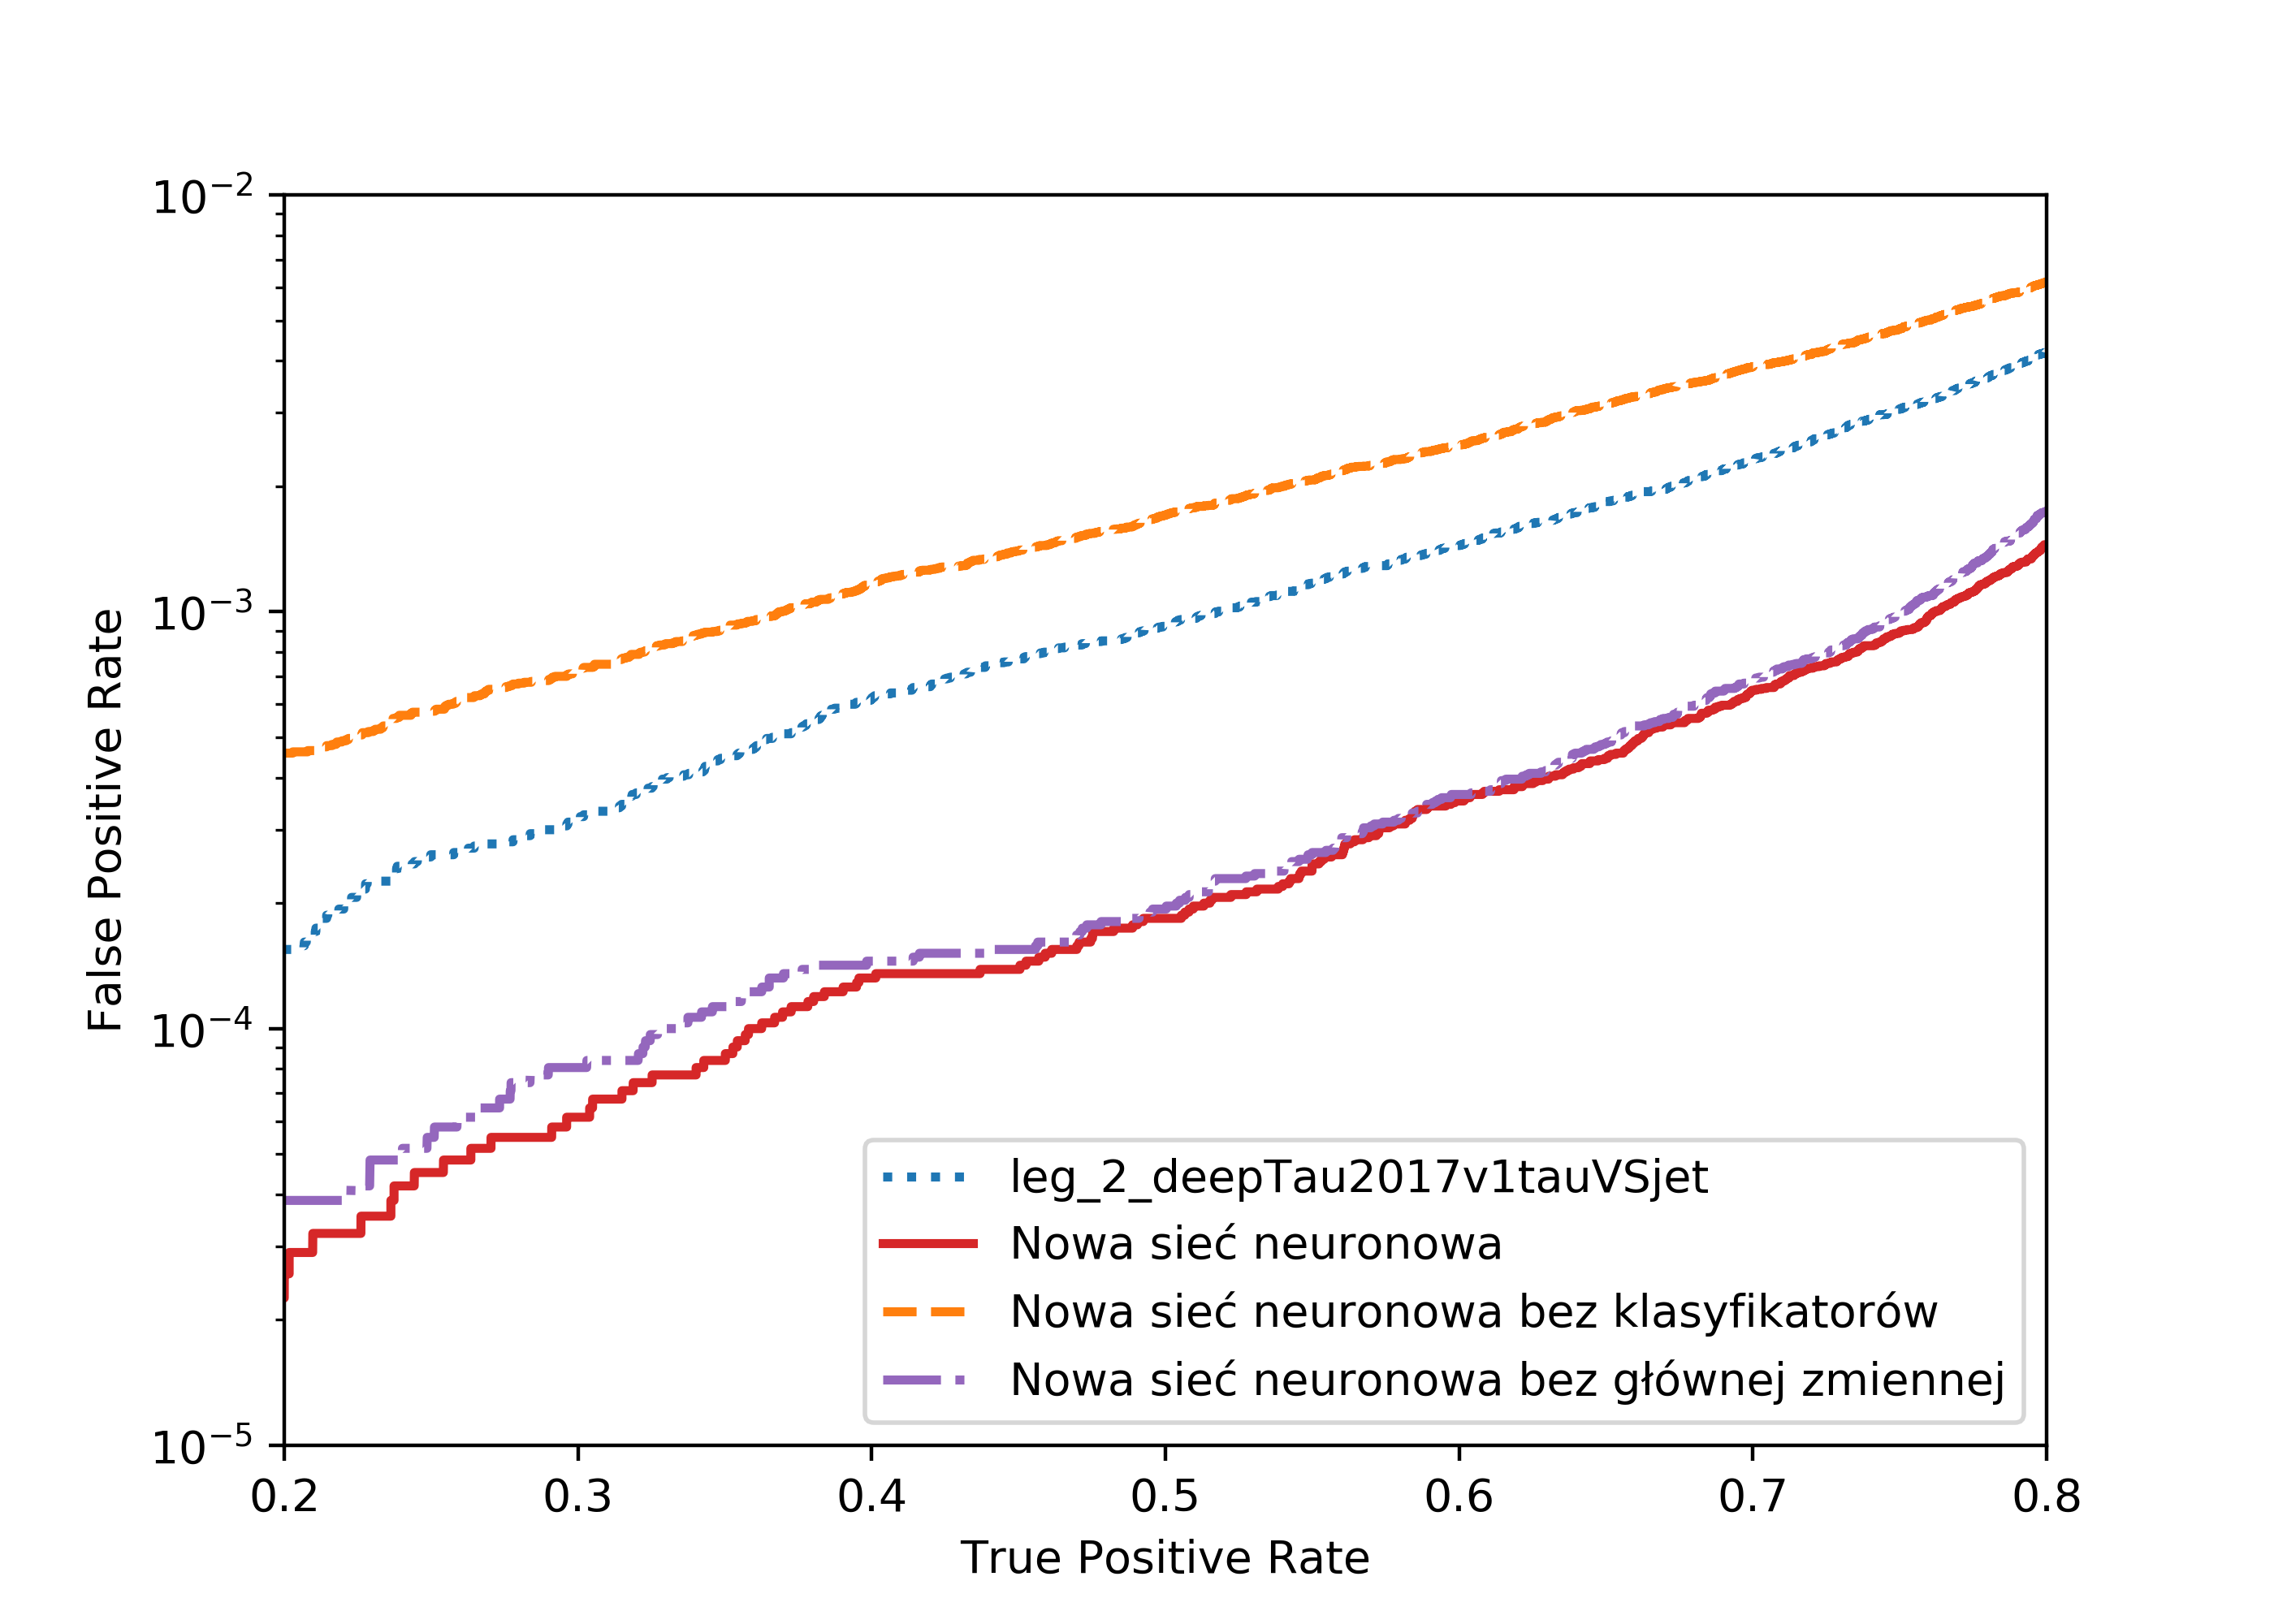
\includegraphics[width=1\textwidth]{new_network.png}
	\caption{Porównanie wszystkich trybów uczenia nowej sieci z najlepszym klasyfikatorem na podstawie krzywej ROC. W nawiasach kwadratowych podano wartość ROC AUC dla danego modelu.}
	\label{fig:res_new}	
	\end{figure}
	
	Na rysunku \ref{fig:res_new} znajdują się wszystkie tryby treningu nowej sieci w porównaniu z \textit{deepTau}. Wyniki dla treningu na pełnych danych i z wyłączeniem głównej zmiennej nie różnią się znacząco, natomiast trening bez klasyfikatorów widocznie pogarsza wygląd krzywej ROC. Na tym fragmencie osiąga gorsze wyniki niż \textit{deepTau}. Jednak patrząc na wartość ROC AUC można podejrzewać, że osiąga lepsze rezultaty na skrajnych fragmentach.
	
	\begin{figure}
	\centering
	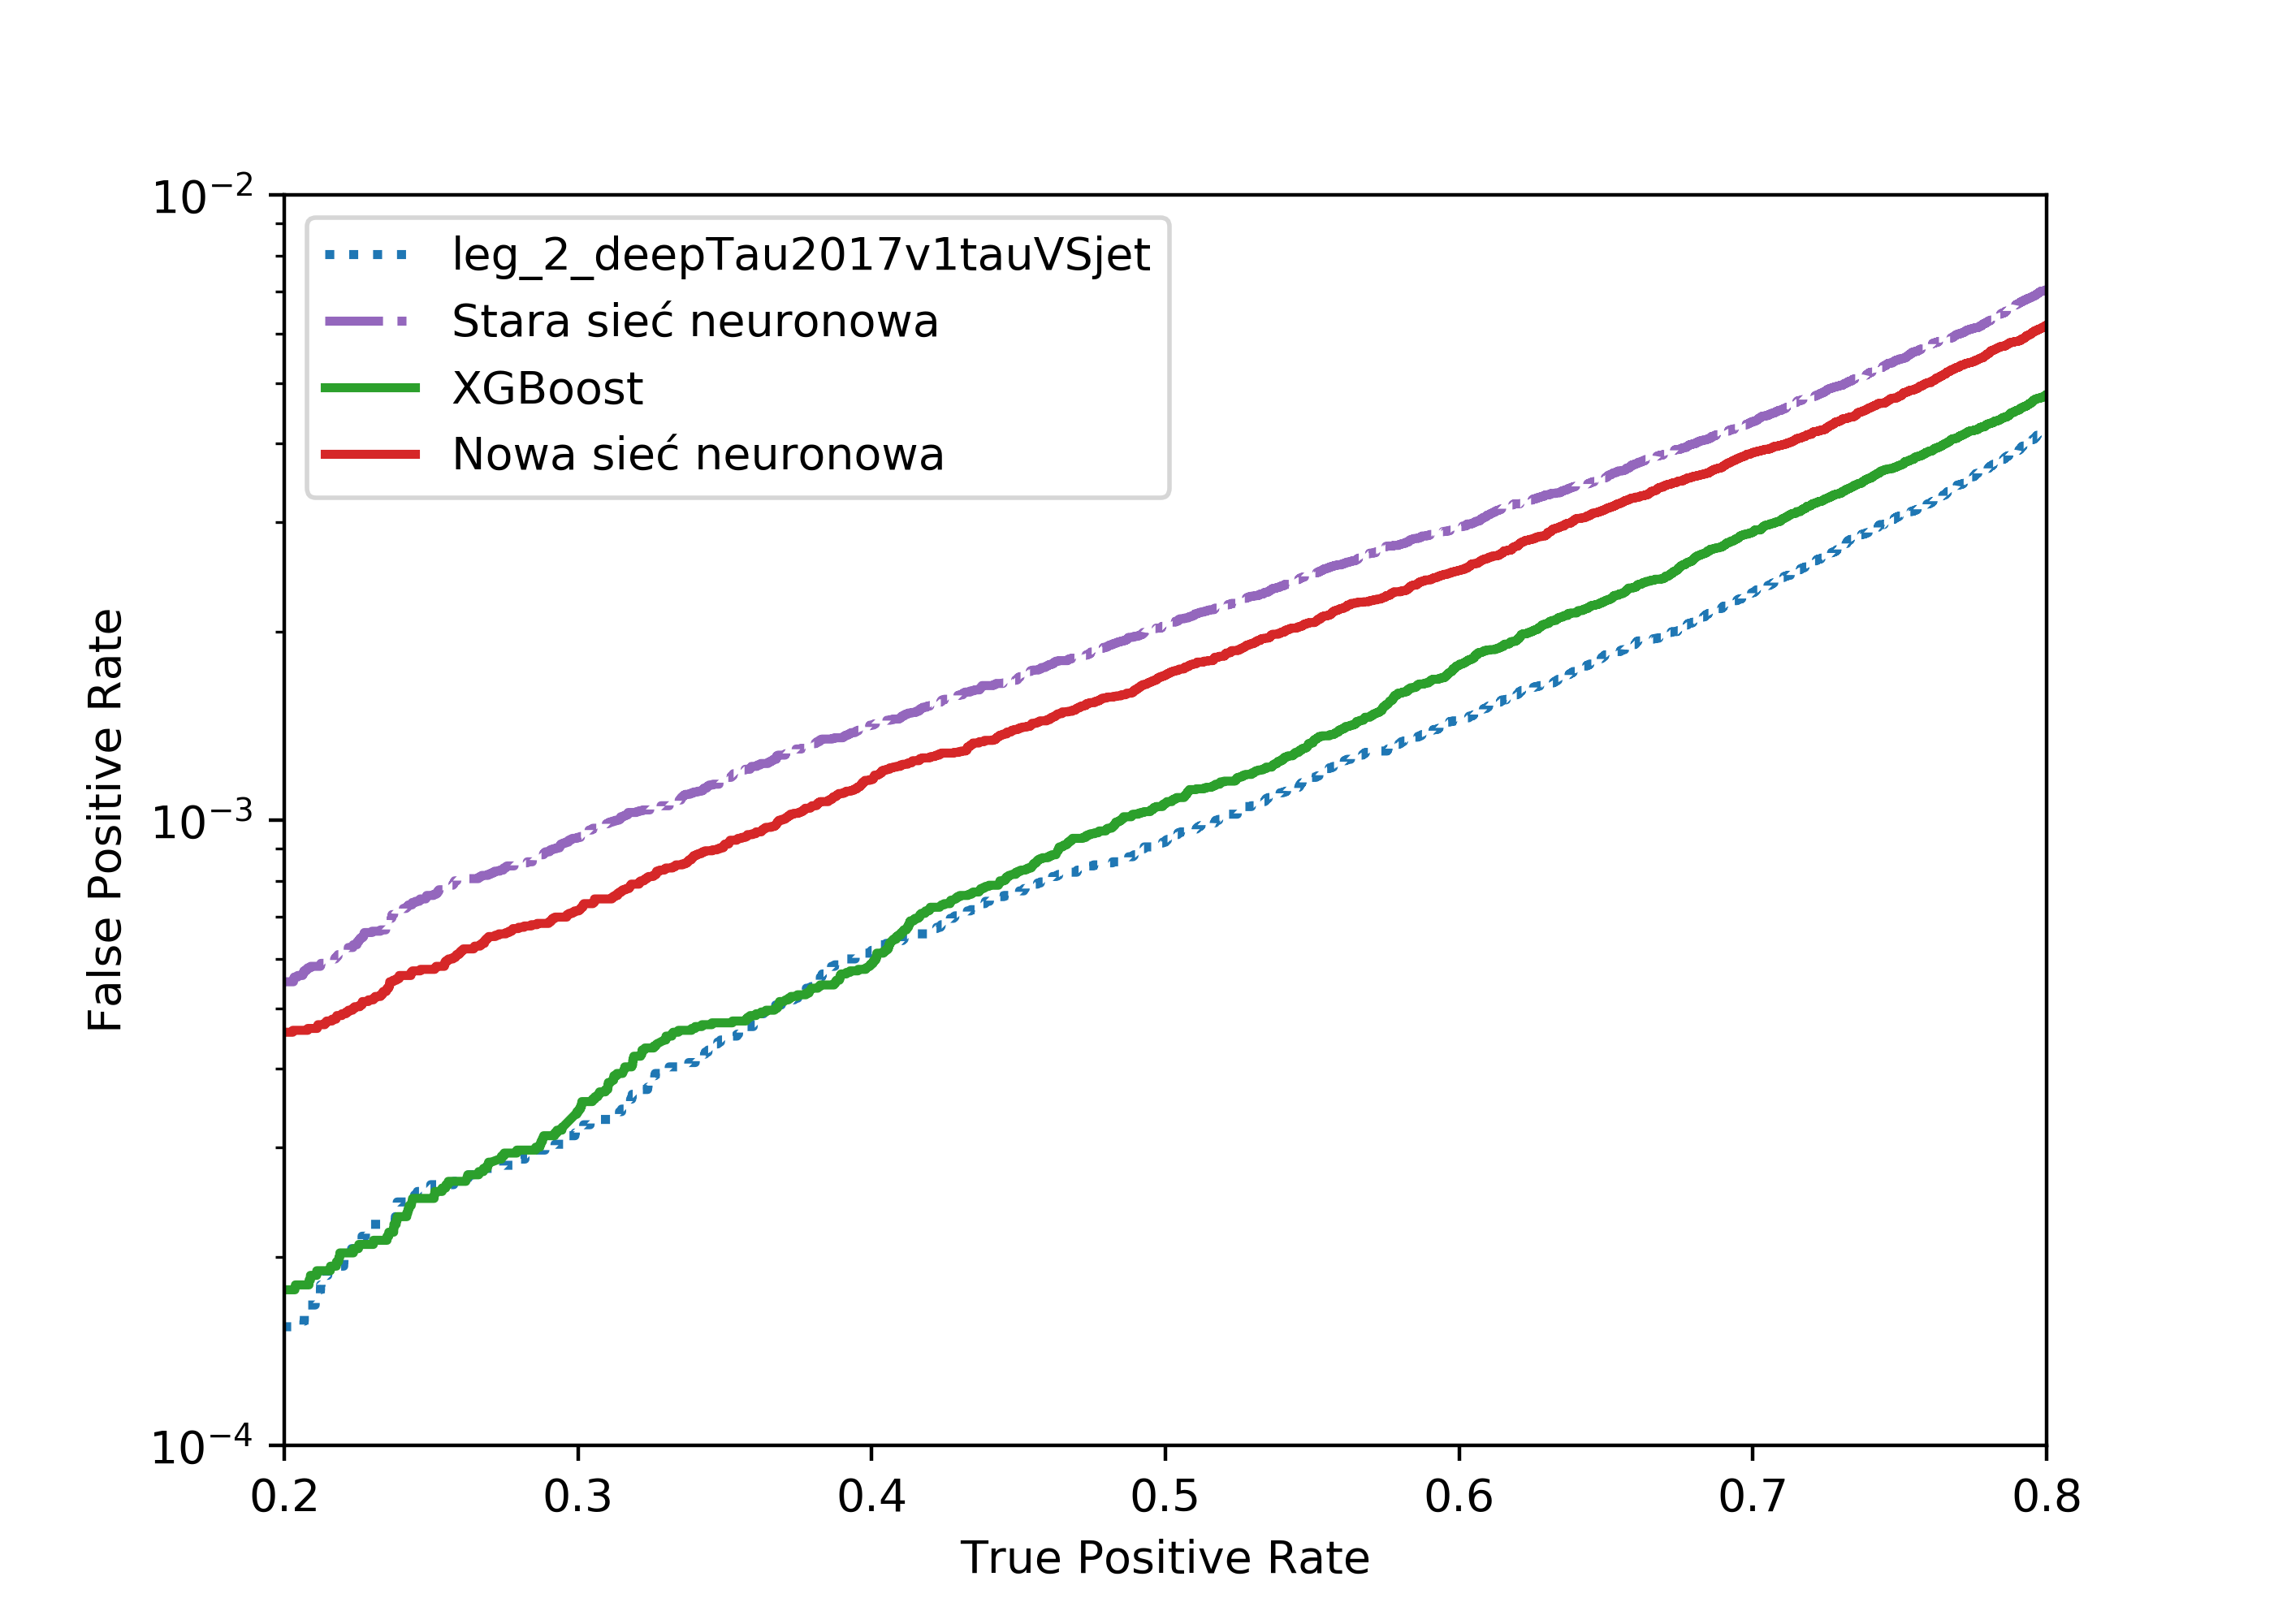
\includegraphics[width=1\textwidth]{without_disc.png}
	\caption{Porównanie modeli uczonych na danych bez klasyfikatorów na podstawie krzywej ROC. W nawiasach kwadratowych podano wartość ROC AUC dla danego modelu.}
	\label{fig:res_disc}
	\end{figure}
	
	Natomiast rysunek \ref{fig:res_disc} pokazuje porównanie każdego typu modelu uczonego na danych bez klasyfikatorów. Dzięki temu można lepiej porównać skuteczność modeli, gdyż każdy z nich uczony był na takich samych danych. Można zauważyć, że na wyróżnionym fragmencie najlepsze wyniki osiąga \textit{deepTau}, jednak są one zbliżone do wyników \textit{XGBoosta}. Patrząc na wartości ROC AUC możemy przypuszczać, że zarówno \textit{XGBoost} jak i \textit{best-nn} uzyskują lepsze rezultaty niż \textit{deepTau} na skrajnych zakresach TPR.
	
    
    \chapter{Dyskusja}
    
	Na podstawie przeprowadzonych eksperymentów najlepszym modelem okazał się \textit{XGBoost}, którego wartość ROC AUC jest lepsza niż wytrenowanych sieci neuronowych oraz wcześniej stosowanych klasyfikatorów. Pomimo małych różnic ROC AUC wszystkie modele wytrenowane na pełnych danych okazały się skuteczniejsze niż wcześniej stosowane klasyfikatory. Najlepiej różnice widać na rysunku \ref{fig:res_best}, gdzie dla założonego TPR, wartości FPR dla \textit{XGBoosta} i \textit{deepTau} różnią się mniej więcej o rząd wielkości.    
    
     Można jednak zauważyć, że krzywa uczenia modeli \textit{baseline} oraz \textit{best-nn} (rysunek \ref{fig:loss}) nie jest całkowicie wypłaszczona. Oznacza to, że trening tych modeli można by wydłużyć o kolejnych kilka epok i potencjalnie poprawić skuteczność modeli.
    
	Warto też wspomnieć, że porównując dane symulacyjne i rzeczywiste widać różnice w rozkładach zmiennych objaśniających, także nie ma pewności, że model dający dobre wyniki na danych symulacyjnych będzie dawał równie dobre wyniki na danych rzeczywistych. Jednakże, sprawdzenie czy modele generalizują się na dane rzeczywiste wykracza poza ramy tej pracy.
	
	Dodatkowo, klasyfikacja odbywała się tylko dla jednego rodzaju tła, czyli dżetów QCD. Należałoby rozszerzyć dane symulacyjne o różne rodzaje tła, aby sytuacja była bardziej zbliżona do danych rzeczywistych.
	
    \chapter{Podsumowanie}
    
	W pracy przedstawiono problem detekcji leptonów $\tau$ przy pomocy modeli uczenia maszynowego. Wprowadzono dwie klasy modeli, sieci neuronowe oraz modele oparte o drzewa decyzyjne. Sprawdzono ich skuteczność oraz porównano ze wcześniej stosowanymi klasyfikatorami. Okazało się, że model oparty na drzewach decyzyjnych (\textit{XGBoost}) osiągnął najlepsze rezultaty. W szczególności wszystkie modele uczone na pełnych danych okazały się lepsze niż wcześniej używane klasyfikatory.
    
    \addcontentsline{toc}{chapter}{Bibliografia}
    \printbibliography
    
\end{document}
